\newglossaryentry{sequence}
{name={\foreignlanguage{greek}{ακολουθία}},
	description={\foreignlanguage{greek}{Μία ακολουθία}\index{\foreignlanguage{greek}{ακολουθία}} 
		\foreignlanguage{greek}{είναι μία διατεταγμένη συλλογή τιμών από ένα σύνολο 
		$\mathcal{A}$. Για παράδειγμα, μία ακολουθία τιμών από το σύνολο 
	   	$\mathcal{A} = \{ \star, \otimes \}$ θα μπορούσε να είναι  
	   	$$ a = \big( \star, \,\otimes, \,\star, \,\star, \,\otimes, \,\ldots \big). $$
	   	Τυπικά, μία ακολουθία $a$ είναι μία} \glsentryuseri{function} \cite{RudinBookPrinciplesMatheAnalysis} 
        		\[
            	a: \mathbb{N} \rightarrow \mathcal{A}: \sampleidx \mapsto a_\sampleidx.
        		\]        
		\foreignlanguage{greek}{Δηλώνουμε μία ακολουθία με $\big( a_{\sampleidx} \big)_{\sampleidx \in \mathbb{N}}$ 
		ή $\big( a^{(\sampleidx)} \big)_{\sampleidx \in \mathbb{N}}$. Μερικές φορές χρησιμοποιούμε  
		και τον συμβολισμό $\big\{ a^{(\sampleidx)} \big\}_{\sampleidx \in \mathbb{N}}$. 
        		Σημείωση ότι η ίδια τιμή $a \in \mathcal{A}$ μπορεί να εμφανιστεί πολλές φορές  
		στην ακολουθία σε διαφορετικές θέσεις $\sampleidx$. 		
        		Οι ακολουθίες είναι θεμελιώδεις για τη μελέτη μεθόδων} \glsentryuserii{ml}, 
        		\foreignlanguage{greek}{για παράδειγμα όταν περιγράφουμε διαδοχικές επαναλήψεις  
        		$\{\weights^{(\iteridx)}\}_{\iteridx \in \mathbb{N}}$ ενός επαναληπτικού} 
		\glsentryuserii{algorithm}. \foreignlanguage{greek}{Μπορούμε επίσης να χρησιμοποιήσουμε μία 
		ακολουθία για να αναπαραστήσουμε ένα άπειρο} \glsentryuseriii{dataset} 
		$$\dataset = \big\{ \pair{\featurevec^{(1)}}{\truelabel^{(1)}},\,\pair{\featurevec^{(2)}}{\truelabel^{(2)}},\,\ldots \big\}.$$ \\
		\foreignlanguage{greek}{Βλέπε επίσης:} \gls{function}, \gls{ml}, \gls{algorithm}, \gls{dataset}. }, 
	first={\foreignlanguage{greek}{ακολουθία}},
	text={\foreignlanguage{greek}{ακολουθία}},
	type=math,
	user1={\foreignlanguage{greek}{ακολουθία}}, %nominative
  	user2={\foreignlanguage{greek}{ακολουθίας}}, %genitive 
	user3={\foreignlanguage{greek}{ακολουθία}}, %accusative
	user4={\foreignlanguage{greek}{ακολουθίες}}, %nominativepl
  	user5={\foreignlanguage{greek}{ακολουθιών}}, %genitivepl 
	user6={\foreignlanguage{greek}{ακολουθίες}} %accusativepl
}

\newglossaryentry{cauchysequence}
{name={\foreignlanguage{greek}{ακολουθία} Cauchy},
	description={\foreignlanguage{greek}{Μία}\index{\foreignlanguage{greek}{ακολουθία} Cauchy} \glsentryuseri{sequence} 
		Cauchy \foreignlanguage{greek}{είναι μία} \glsentryuseri{sequence}
		$\big( \featurevec^{(\sampleidx)}\big)_{\sampleidx \in \mathbb{N}}$ 
		\foreignlanguage{greek}{σε έναν} \glsentryuseriii{metricspace} $\pair{\featurespace}{\metric{\cdot}{\cdot}}$  
		\foreignlanguage{greek}{έτσι ώστε τα στοιχεία $\featurevec^{(\sampleidx)}\in \featurespace$ 
		γίνονται τελικά αυθαίρετα κοντινά το ένα στο άλλο.
		Με άλλα λόγια,} \cite[Def. 3.8]{RudinBookPrinciplesMatheAnalysis}, 
		\[
		\forall \epsilon > 0, \exists N \in \mathbb{N} \text{ \foreignlanguage{greek}{έτσι ώστε} } 
		\forall \sampleidx, \sampleidx' \geq N, \ \metric{\featurevec^{(\sampleidx)}}{\featurevec^{(\sampleidx')}} < \epsilon.
		\] 
		\foreignlanguage{greek}{Το Σχ.}\ \ref{fig:fpit_cauchy_sqrt2_dict} \foreignlanguage{greek}{δείχνει μία} \glsentryuseriii{sequence} 
		Cauchy \foreignlanguage{greek}{στον} \glsentryuseriii{metricspace} $\pair{\mathbb{Q}}{|\cdot|}$ 
		\foreignlanguage{greek}{ρητών αριθμών.}
		\begin{figure}[H]
			\centering
		  	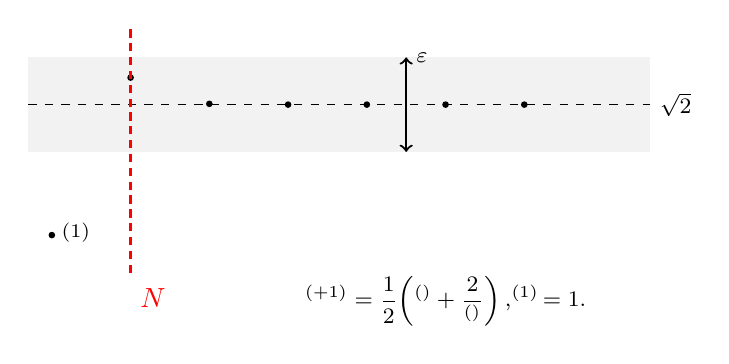
\begin{tikzpicture}[x=1cm,y=4cm]
			% Parameters
			\def\srtwo{1.4142}
			\def\eps{0.15}
			\def\nmax{7}
			% Axes
			% \draw[->] (-0.3,0) -- (\nmax+0.6,0) node[right] {$\sampleidx$};
			% \draw[->] (-0.3,0.9) -- (-0.3,1.46) node[above] {$x^{(\sampleidx)}$};
			% epsilon band around sqrt(2)
			\fill[gray!30, opacity=0.35]
			(-0.3,{\srtwo-\eps}) rectangle (\nmax+0.6,{\srtwo+\eps});
			%	\draw[dotted] (-0.3,{\srtwo+\eps}) -- (\nmax+0.6,{\srtwo+\eps})
			%	node[right] {\footnotesize{$\sqrt{2}+\varepsilon$}};
			%	\draw[dotted] (-0.3,{\srtwo-\eps}) -- (\nmax+0.6,{\srtwo-\eps})
			%	node[right] {\footnotesize{$\sqrt{2}-\varepsilon$}};
			% Double arrow showing epsilon band width
			\draw[<->, thick] (4.5,{\srtwo-\eps}) -- (4.5,{\srtwo+\eps})
			node[above, right] {\footnotesize{$\varepsilon$}};
			% Limit line at sqrt(2)
			\draw[dashed] (-0.3,\srtwo) -- (\nmax+0.6,\srtwo)
			node[right] {\footnotesize{$\sqrt{2}$}};
			% Sequence via fixed-point iteration: x_{n+1} = 0.5(x_n + 2/x_n), x_0 = 1
			% Replace the foreach loop by:
			\fill (0,1.0000) circle (1.2pt) node [right] {$\feature^{(1)}$};
			\fill (1,1.5000) circle (1.2pt);
			\fill (2,1.4167) circle (1.2pt);
			\fill (3,1.4142) circle (1.2pt);
			\fill (4,1.41421) circle (1.2pt);
			\fill (5,1.4142136) circle (1.2pt);
			\fill (6,1.41421356) circle (1.2pt);
			% Choose an N (first index within eps-band) -- here N=3 works for eps=0.005
			\def\N{1}
			\draw[densely dashed, thick, red] (\N,0.88) -- (\N,1.655);
			\node[right, red] at (\N,0.8) {$N$};
			% Formula box (fixed-point iteration)
			\node[align=right, anchor=north, font=\small]
			at (5,0.9)
			{\footnotesize{$\displaystyle \feature^{(\sampleidx+1)}=\frac{1}{2}\!\left(\feature^{(\sampleidx)}+\frac{2}{\feature^{(\sampleidx)}}\right), \feature^{(1)}=1.$}};
			% Optional: annotate a few rational iterates
			%	\node[font=\scriptsize, anchor=west] at (0,1.5-0.06) {$x^{(1)}=\tfrac{3}{2}$};
			%	\node[font=\scriptsize, anchor=west] at (1,1.5-0.12) {$x^{(2)}=\tfrac{17}{12}$};
			%	\node[font=\scriptsize, anchor=west] at (2,1.5-0.145) {$x^{(3)}=\tfrac{577}{408}$};
			\end{tikzpicture}
		{\selectlanguage{greek}
		\caption{\foreignlanguage{greek}{Μία} \glsentryuseri{sequence} \selectlanguage{english}{Cauchy} 
			$\big(\feature^{(\sampleidx)}\big)_{\sampleidx\in\mathbb{N}}$ 
			\foreignlanguage{greek}{στον} \glsentryuseriii{metricspace} $\pair{\mathbb{Q}}{|\cdot|}$. 
			\foreignlanguage{greek}{Αυτή η} \glsentryuseri{sequence} \foreignlanguage{greek}{παράγεται από μία} 
			\gls{fixedpointiter} \foreignlanguage{greek}{που χρησιμοποιείται για την προσέγγιση του} 
			$\sqrt{2}$. \foreignlanguage{greek}{Για όλα τα $\sampleidx \ge N$, τα στοιχεία της} \glsentryuserii{sequence} 
			\foreignlanguage{greek}{βρίσκονται εντός μίας ζώνης πλάτους $\varepsilon$. 
			Σημείωση ότι η} \glsentryuseri{sequence} \foreignlanguage{greek}{δεν συγκλίνει στον $\mathbb{Q}$, 
			εφόσον} $\sqrt{2} \notin \mathbb{Q}$ \cite[\foreignlanguage{greek}{Παράδειγμα} 1.1]{RudinBookPrinciplesMatheAnalysis}.\label{fig:fpit_cauchy_sqrt2_dict}} }
		\end{figure}
		\foreignlanguage{greek}{Βλέπε επίσης:} \gls{sequence}, \gls{metricspace}, \gls{fixedpointiter}. }, 
	first={\foreignlanguage{greek}{ακολουθία} Cauchy},
	text={\foreignlanguage{greek}{ακολουθία} Cauchy},
	type=math,
	user1={\foreignlanguage{greek}{ακολουθία} Cauchy}, %nominative
  	user2={\foreignlanguage{greek}{ακολουθίας} Cauchy}, %genitive 
	user3={\foreignlanguage{greek}{ακολουθία} Cauchy} %accusative
}

\newglossaryentry{algconn}
{name={\foreignlanguage{greek}{αλγεβρική συνεκτικότητα}},
	description={\foreignlanguage{greek}{Η αλγεβρική συνεκτικότητα}\index{\foreignlanguage{greek}{αλγεβρική συνεκτικότητα}} 
		(algebraic connectivity) \foreignlanguage{greek}{ενός} \glsentryuserii{undirectedgraph} 
		\foreignlanguage{greek}{είναι η δεύτερη μικρότερη} \glsentryuseri{eigenvalue} $\eigval{2}$ 
		\foreignlanguage{greek}{του} \glsentryuserii{LapMat} \foreignlanguage{greek}{του}. 
		\foreignlanguage{greek}{Ένας} \glsentryuseri{undirectedgraph} \foreignlanguage{greek}{είναι} 
		\glsentryuseri{connected} \foreignlanguage{greek}{αν και μόνο αν} $\eigval{2} >0$ 
		(\foreignlanguage{greek}{βλέπε Σχ.} \ref{fig_algconn_dict}) \cite{ChungSpecGraphTheory}, \cite{Spielman2019}. 
		\begin{figure}[H]
			\centering
			\begin{tikzpicture}
			% Horizontal axis
			\draw[->,line width=1pt] (-1, -1) -- (9, -1) node[below] {$\eigval{2}$};
			% Ticks on the horizontal axis
			\draw[thick] (0, -0.8) -- (0, -1.2) node[below] {{$\eigval{2}\!=\!0$}};
			%\draw[thick] (7, -0.8) -- (7, -1.2) node[below] {$\eigval{2}\!=\!\nrnodes$};
			\draw[thick] (7, -0.8) -- (7, -1.2) node[below] {$\eigval{2}\!=\! 3$};
			% }\!=\!\nrnodes = 3 in this specific case
			\draw[thick] (3.5, -0.8) -- (3.5, -1.2) node[below] {$\eigval{2}\!=\! 1$};
			% could make sense to add this explicitly for the second example, too
			% Left graph (single edge)
			\node[circle, fill=black, inner sep=1.5pt, label=above:{1}] (A1) at (0, 1.5) {};
			\node[above=0.5cm of A1, align=center] {\mbox{\foreignlanguage{greek}{μη συνεκτικός}}};
			\node[circle, fill=black, inner sep=1.5pt, label=below right:{2}] (B1) [below right=0.8cm and 0.5cm of A1] {};
			\node[circle, fill=black, inner sep=1.5pt, label=below left:{3}] (C1) [below left=0.8cm and 0.5cm of A1] {};
			\draw [line width=1 pt]  (A1) -- (B1);
			% Middle graph (two edges, shifted right)
			\begin{scope}[xshift=3.5cm]
				\node[circle, fill=black, inner sep=1.5pt, label=above:{1}] (A2) at (0, 1.5) {};
				\node[above=0.5cm of A2, align=center] {\mbox{\glsentryuseri{connected}}};
				\node[circle, fill=black, inner sep=1.5pt, label=below right:{2}] (B2) [below right=0.8cm and 0.5cm of A2] {};
				\node[circle, fill=black, inner sep=1.5pt, label=below left:{3}] (C2) [below left=0.8cm and 0.5cm of A2] {};
				\draw [line width=1 pt]  (A2) -- (B2);
				\draw [line width=1 pt]  (B2) -- (C2);
			\end{scope}
			% Right graph (three edges, shifted further right)
			\begin{scope}[xshift=7cm]
				\node[circle, fill=black, inner sep=1.5pt, label=above:{1}] (A3) at (0, 1.5) {};
				\node[above=0.5cm of A3, align=center] {\mbox{\foreignlanguage{greek}{πλήρης} \glsentryuseri{graph}}};
				\node[circle, fill=black, inner sep=1.5pt, label=below right:{2}] (B3) [below right=0.8cm and 0.5cm of A3] {};
				\node[circle, fill=black, inner sep=1.5pt, label=below left:{3}] (C3) [below left=0.8cm and 0.5cm of A3] {};
				\draw [line width=1 pt] (A3) -- (B3);
				\draw [line width=1 pt]  (B3) -- (C3);
				\draw [line width=1 pt]  (A3) -- (C3);
			\end{scope}
			\end{tikzpicture}
		{\selectlanguage{greek}
		\caption{\foreignlanguage{greek}{Τρία παραδείγματα} \glsentryuserv{undirectedgraph}. \label{fig_algconn_dict}} }
		\end{figure}
		\foreignlanguage{greek}{Βλέπε επίσης:} \gls{undirectedgraph}, \gls{eigenvalue}, \gls{LapMat}, \gls{connected}, \gls{graph}.},
	first={\foreignlanguage{greek}{αλγεβρική συνεκτικότητα}},
	text={\foreignlanguage{greek}{αλγεβρική συνεκτικότητα}},
	type=math,
	user1={\foreignlanguage{greek}{αλγεβρική συνεκτικότητα}}, %nominative
  	user2={\foreignlanguage{greek}{αλγεβρικής συνεκτικότητας}}, %genitive 
	user3={\foreignlanguage{greek}{αλγεβρική συνεκτικότητα}} %accusative
}

\newglossaryentry{svd}
{name={\foreignlanguage{greek}{ανάλυση ιδιαζουσών τιμών}}, 
  	description={\foreignlanguage{greek}{Η ανάλυση ιδιαζουσών τιμών}\index{\foreignlanguage{greek}{ανάλυση ιδιαζουσών τιμών}} 
		(singular value decomposition - SVD) \foreignlanguage{greek}{για έναν} \glsentryuseriii{matrix} 
		$\mA \in \mathbb{R}^{\samplesize \times \dimlocalmodel}$ \foreignlanguage{greek}{είναι μία παραγοντοποί\-ηση της 
		ακόλουθης μορφής: $$\mA = \mathbf{V} {\bm \Lambda} \mathbf{U}\,^{T}$$ με ορθοκανονικούς} \glsentryuservi{matrix} 
		$\mV = \big(\vv^{(1)},\,\ldots,\,\vv^{(\samplesize)}\big) \in \mathbb{R}^{\samplesize \times \samplesize}$ \foreignlanguage{greek}{και} 
		$\mU = \big( \vu^{(1)},\,\ldots,\,\vu^{(\dimlocalmodel)} \big) \in \mathbb{R}^{\dimlocalmodel \times \dimlocalmodel}$  
		\cite{GolubVanLoanBook} (\foreignlanguage{greek}{βλέπε Σχ.} \ref{fig_svd_dict}). 
		\begin{figure}[H]
		 	\centering	
		 	\begin{tikzpicture}[>=latex, line cap=round, line join=round, scale=1]
		 	\def\xL{0}
		 	\def\xR{6}
		 	\def\len{2.0}
		 	\def\sone{1.6}
		 	\def\stwo{0.7}
		 	\draw[thick,->] (\xL,0) -- ++(\len,0) node[midway,below] {$\vu^{(1)}$};
			\draw[thick,->] (\xL,0) -- ++(0,\len) node[midway,left] {$\vu^{(2)}$};
			\draw[dashed,->] (\xL+2.9,0) -- (\xR-0.9,0);
			\begin{scope}[shift={(\xR+0.5,0)},rotate=30]
			\draw[thick,->] (0,0) -- (\sone*\len,0) node[pos=1,right] {$\lambda_1 \vv^{(1)}$};
			\draw[thick,->] (0,0) -- (0,\stwo*\len) node[pos=1,above] {$\lambda_2 \vv^{(2)}$};
			\end{scope}
		 	\end{tikzpicture}
		{\selectlanguage{greek}
		\caption{\foreignlanguage{greek}{Ορθοκανονικοί} \glsentryuseriv{matrix} $\mV$ \foreignlanguage{greek}{και} $\mU$. \label{fig_svd_dict} } }
		\end{figure}
		\foreignlanguage{greek}{Ο} \glsentryuseri{matrix} ${\bm \Lambda} \in \mathbb{R}^{\samplesize \times \dimlocalmodel}$ 
		\foreignlanguage{greek}{είναι μη μηδενικός μόνο κατά την κύρια διαγώνιο, της οποίας οι καταχωρίσεις 
		$\Lambda_{\featureidx,\featureidx}$ είναι μη αρνητικές και αναφέρονται ως} \glsentryuseriv{singularvalue}.
		\\
		\foreignlanguage{greek}{Βλέπε επίσης:} \gls{matrix}, \gls{singularvalue}. },
	first={\foreignlanguage{greek}{ανάλυση ιδιαζουσών τιμών}},
	text={\foreignlanguage{greek}{ανάλυση ιδιαζουσών τιμών}},
	type=math,
	user1={\foreignlanguage{greek}{ανάλυση ιδιαζουσών τιμών}}, %nominative
	user2={\foreignlanguage{greek}{ανάλυσης ιδιαζουσών τιμών}} %genitive  
}

\newglossaryentry{evd}
{name={\foreignlanguage{greek}{ανάλυση ιδιοτιμών}}, 
	description={\foreignlanguage{greek}{Η ανάλυση ιδιοτιμών}\index{\foreignlanguage{greek}{ανάλυση ιδιοτιμών}} 
		(eigenvalue decomposition - EVD) \foreignlanguage{greek}{για έναν τετραγωνικό} \glsentryuseriii{matrix} 
		$\mA \in \mathbb{R}^{\dimlocalmodel \times \dimlocalmodel}$ \foreignlanguage{greek}{είναι μία παραγοντοποίηση 
		της μορφής $$\mA = \mathbf{V} {\bm \Lambda} \mathbf{V}^{-1}.$$ 
		Οι στήλες του} \glsentryuserii{matrix} $\mV = \big( \vv^{(1)}, \,\ldots, \,\vv^{(\dimlocalmodel)} \big)$ \foreignlanguage{greek}{είναι τα}  
		\glsentryuseriv{eigenvector} \foreignlanguage{greek}{του} \glsentryuserii{matrix} $\mV$. \foreignlanguage{greek}{Ο διαγώνιος}   
		\glsentryuseri{matrix} ${\bm \Lambda} = {\rm diag} \big\{ \eigval{1}, \,\ldots, \,\eigval{\dimlocalmodel} \big\}$ 
		\foreignlanguage{greek}{περιέχει τις} \glsentryuservi{eigenvalue} $\eigval{\featureidx}$ \foreignlanguage{greek}{που αντιστοιχούν στα} 
		\glsentryuservi{eigenvector} $\vv^{(\featureidx)}$. \foreignlanguage{greek}{Σημείωση ότι η παραπάνω ανάλυση υφίσταται μόνο αν ο} 
		\glsentryuseri{matrix} $\mA$ \foreignlanguage{greek}{είναι διαγωνοποιήσιμος.} \\
		\foreignlanguage{greek}{Βλέπε επίσης:} \gls{matrix}, \gls{eigenvector}, \gls{eigenvalue}.},
	first={\foreignlanguage{greek}{ανάλυση ιδιοτιμών}},
	text={\foreignlanguage{greek}{ανάλυση ιδιοτιμών}},
	type=math,
	user1={\foreignlanguage{greek}{ανάλυση ιδιοτιμών}}, %nominative
	user2={\foreignlanguage{greek}{ανάλυσης ιδιοτιμών}}, %genitive
	user3={\foreignlanguage{greek}{ανάλυση ιδιοτιμών}} %accusative   
}

\newglossaryentry{transpose}
{name={\foreignlanguage{greek}{ανάστροφος}},
	description={\foreignlanguage{greek}{Η ανάστροφος} (transpose)\index{\foreignlanguage{greek}{ανάστροφος}} 
		\foreignlanguage{greek}{ενός} \glsentryuserii{matrix} \foreignlanguage{greek}{πραγματικής τιμής προκύπτει με την 
		ανταλλαγή γραμμών και στηλών. Για έναν} \glsentryuseriii{matrix} $\mA \in \mathbb{R}^{\samplesize \times \nrfeatures}$, 
		\foreignlanguage{greek}{η ανάστροφός του δηλώνεται με $\mA^{T}$ και ικανοποιεί} 
		$\big(\mA^{T}\big)_{\featureidx,\featureidx'}=\mA_{\featureidx',\featureidx}$.
		\\
		\foreignlanguage{greek}{Βλέπε επίσης:} \gls{matrix}, \gls{symmetricmatrix}. },
 	first={\foreignlanguage{greek}{ανάστροφος}},
 	text={\foreignlanguage{greek}{ανάστροφος}},
	type=math,
	user1={\foreignlanguage{greek}{ανάστροφος}}, %nominative
  	user2={\foreignlanguage{greek}{ανάστροφου}}, %genitive 
	user3={\foreignlanguage{greek}{ανάστροφο}} %accusative
 }

\newglossaryentry{iid}
{name={\foreignlanguage{greek}{ανεξάρτητες και ταυτόσημα κατανεμημένες}}, 
	description={\foreignlanguage{greek}{Μία συλλογή} \glsentryuserv{rv} $\datapoint^{(1)}, \,\ldots, \,\datapoint^{(\samplesize)}$ 
		\foreignlanguage{greek}{αναφέρεται ως ανεξάρτητη και ταυτόσημα κατανεμημένη}
		(independent and identically distributed - i.i.d.)\index{\foreignlanguage{greek}{ανεξάρτητες και ταυτόσημα κατανεμημένες}} 
		\foreignlanguage{greek}{αν κάθε $\datapoint^{(\sampleidx)}$ ακολουθεί την ίδια} \glsentryuseriii{probdist},  
		\foreignlanguage{greek}{και οι} \glsentryuseriv{rv} \foreignlanguage{greek}{είναι αμοιβαία ανεξάρτητες. 
		Για την ακρίβεια, για οποιαδήποτε συλλογή} \glsentryuserv{event} $\mathcal{A}_1, \,\ldots, \,\mathcal{A}_\samplesize$, 
		\foreignlanguage{greek}{έχουμε}
       		\[
          		\prob{ \datapoint^{(1)} \in \mathcal{A}_1, \,\ldots, \,\datapoint^{(\samplesize)} \in \mathcal{A}_{\samplesize}} 
         		= \prod_{\sampleidx=1}^{\samplesize} \prob{ \datapoint^{(\sampleidx)} \in \mathcal{A}_\sampleidx}.
         	\] \\
		\foreignlanguage{greek}{Βλέπε επίσης:} \gls{probdist}, \gls{rv}, \gls{event}, \gls{datapoint}, \gls{iidasspt}.},
	first={\foreignlanguage{greek}{ανεξάρτητες και ταυτόσημα κατανεμημένες}},
	text={\foreignlanguage{greek}{ανεξάρτητες και ταυτόσημα κατανεμημένες}},
	type=math,
	user1={\foreignlanguage{greek}{ανεξάρτητες και ταυτόσημα κατανεμημένες}}, %nominativepl
  	user2={\foreignlanguage{greek}{ανεξάρτητων και ταυτόσημα κατανεμημένων}}, %genitivepl  
	user3={\foreignlanguage{greek}{ανεξάρτητες και ταυτόσημα κατανεμημένες}} %accusativepl 
}
\newglossaryentry{markovsinequality}
{name={\foreignlanguage{greek}{ανισότητα του} Markov},
	description={TBC.\index{Markov’s inequality} },
	first={\foreignlanguage{greek}{ανισότητα του} Markov},
    	text={\foreignlanguage{greek}{ανισότητα του} Markov},
	type=math,
	user1={\foreignlanguage{greek}{ανισότητα του} Markov}, %nominative 
	user2={\foreignlanguage{greek}{ανισότητας του} Markov}, %genitive   
	user3={\foreignlanguage{greek}{ανισότητα του} Markov} %accusative
}

\newglossaryentry{concentrationinequ}
{name={\foreignlanguage{greek}{ανισότητα συγκέντρωσης}}, 
	description={\foreignlanguage{greek}{Η ανισότητα συγκέντρωσης} (concentration inequality) 
		\foreignlanguage{greek}{αναφέρεται σε ένα άνω φράγμα της} 
		\glsentryuserii{probability}\index{\foreignlanguage{greek}{ανισότητα συγκέντρωσης}} 
		\foreignlanguage{greek}{ότι μία} \glsentryuseri{rv} \foreignlanguage{greek}{αποκλίνει περισσότερο 
		από ένα καθορισμένο ποσό από την} \glsentryuseriii{expectation} \foreignlanguage{greek}{της} \cite{Wain2019}.  
		\\
		\foreignlanguage{greek}{Βλέπε επίσης:} \gls{probability}, \gls{rv}, \gls{expectation}, \gls{markovsinequality}, \gls{chebyshevsinequality}, 
		\gls{hoeffdingsinequality}, \gls{chernoffbound}.}, 
	first={\foreignlanguage{greek}{ανισότητα συγκέντρωσης}}, 
	text={\foreignlanguage{greek}{ανισότητα συγκέντρωσης}},
	type=math,
	user1={\foreignlanguage{greek}{ανισότητα συγκέντρωσης}}, %nominative 
	user2={\foreignlanguage{greek}{ανισότητας συγκέντρωσης}}, %genitive   
	user3={\foreignlanguage{greek}{ανισότητα συγκέντρωσης}} %accusative
}

\newglossaryentry{chebyshevsinequality}
{name={\foreignlanguage{greek}{ανισότητα του} Chebyshev},
	description={TBC.\index{Chebyshev’s inequality} },
    	first={\foreignlanguage{greek}{ανισότητα του} Chebyshev},
     	text={\foreignlanguage{greek}{ανισότητα του} Chebyshev},
	type=math,  
	user1={\foreignlanguage{greek}{ανισότητα του} Chebyshev}, %nominative 
	user2={\foreignlanguage{greek}{ανισότητας του} Chebyshev}, %genitive   
	user3={\foreignlanguage{greek}{ανισότητα του} Chebyshev} %accusative
}

\newglossaryentry{hoeffdingsinequality}
{name={\foreignlanguage{greek}{ανισότητα του} Hoeffding},
	description={TBC.\index{Hoeffding's inequality} },
    	first={\foreignlanguage{greek}{ανισότητα του} Hoeffding},
    	text={\foreignlanguage{greek}{ανισότητα του} Hoeffding},
	type=math,   
	user1={\foreignlanguage{greek}{ανισότητα του} Hoeffding}, %nominative 
	user2={\foreignlanguage{greek}{ανισότητας του} Hoeffding}, %genitive   
	user3={\foreignlanguage{greek}{ανισότητα του} Hoeffding} %accusative
}

\newglossaryentry{inverse}
{name={\foreignlanguage{greek}{αντίστροφος πίνακας}},
	description={\foreignlanguage{greek}{Ένας αντίστροφος} \glsentryuseri{matrix}\index{\foreignlanguage{greek}{αντίστροφος πίνακας}} 
		(inverse matrix) $\mA^{-1}$ \foreignlanguage{greek}{ορίζεται για έναν τετραγωνικό} \glsentryuseriii{matrix}  
 		$\mA \in \mathbb{R}^{n \times n}$ \foreignlanguage{greek}{που είναι} \glsentryuseri{fullrank}, \foreignlanguage{greek}{που σημαίνει 
		ότι οι στήλες του είναι} \glsentryuseriii{linearlyindep}. \foreignlanguage{greek}{Σε αυτή την περίπτωση, ο $\mA$ λέγεται ότι 
		είναι αντιστρέψιμος, και ο αντίστροφός του ικανοποιεί 
 		\[
 		\mA \mA^{-1} = \mA^{-1} \mA = \mI.
 		\]  	
     		Ένας τετραγωνικός} \glsentryuseri{matrix} \foreignlanguage{greek}{είναι αντιστρέψιμος αν και μόνο αν η} \glsentryuseriv{det} 
		\foreignlanguage{greek}{του είναι μη μηδενική. Οι αντίστροφοι} \glsentryuseriv{matrix} \foreignlanguage{greek}{είναι θεμελιώδεις 
		στη λύση συστημάτων γραμμικών εξισώσεων και στην κλειστής μορφής λύση} \glsentryuserii{linreg} \cite{Strang2007}, \cite{Horn91}. 
		\foreignlanguage{greek}{Η έννοια ενός αντίστροφου} \glsentryuserii{matrix} \foreignlanguage{greek}{μπορεί να επεκταθεί σε} 
		\glsentryuservi{matrix} \foreignlanguage{greek}{που δεν είναι τετραγωνικοί ή} \glsentryuseri{fullrank}. 
		\foreignlanguage{greek}{Μπορεί κανείς να ορίσει έναν \guillemotleft αριστερό αντίστροφο\guillemotright\ $\mB$ 
     		που ικανοποιεί $\mB \mA = \mI$ ή έναν \guillemotleft δεξιό αντίστροφο\guillemotright\ $\mC$ που 
		ικανοποιεί $\mA \mC = \mI$. Για γενικούς ορθογώνιους ή ιδιάζοντες} \glsentryuservi{matrix}, \foreignlanguage{greek}{ο} 
     		\glsentryuseri{pseudoinverse} Moore–Penrose $\mA^{+}$ \foreignlanguage{greek}{παρέχει μία ενοποιημένη έννοια 
		ενός γενικευμένου αντίστροφου} \glsentryuserii{matrix} \cite{GolubVanLoanBook}.
 		 \begin{figure}[H]
 			\centering
 			\begin{tikzpicture}[x=2cm,y=2cm]
 			% LEFT: Standard basis
 			\begin{scope}
 				\draw[->, thick] (0,0) -- (1,0) node[below right] {$\vx$};
 				\draw[->, thick] (0,0) -- (0,1) node[above left] {$\vy$};
 			\end{scope}
 			% CENTER: Transformed basis (by A)
 			\begin{scope}[shift={(2.0,0)}]
 				\coordinate (A) at (1.5,0.5);
 				\coordinate (B) at (-0.2,1.2);
				\draw[->, very thick, red] (0,0) -- (A) node[pos=0.5, below right] {$\mA \vx$};
 				\draw[->, very thick, red] (0,0) -- (B) node[above right] {$\mA \vy$};
 			\end{scope}
 			% RIGHT: Inverse transformation
 			\begin{scope}[shift={(4.9,0)}]
 				\draw[->, very thick, blue] (0,0) -- (1,0) node[pos=0.5, below] {$\mA^{-1} (\mA \vx) = \vx$};
 				\draw[->, very thick, blue] (0,0) -- (0,1) node[above] {$\mA^{-1} (\mA \vy) = \vy$};
 			\end{scope}
 			% Curved arrows between stages
 			\draw[->, thick, bend left=20] (1.2,0.4) to node[above] {$\mA$} (1.8,0.4);
 			\draw[->, thick, bend left=20] (3.8,0.4) to node[below] {$\mA^{-1}$} (4.4,0.4);
 			\end{tikzpicture}
			{\selectlanguage{greek}
 			\caption{\foreignlanguage{greek}{Ένας} \glsentryuseri{matrix} $\mathbf{A}$ \foreignlanguage{greek}{αναπαριστά έναν 
			γραμμικό μετασχηματισμό του $\mathbb{R}^{2}$. Ο αντίστροφος} \glsentryuseri{matrix} $\mathbf{A}^{-1}$ 
			\foreignlanguage{greek}{αναπαριστά τον αντίστροφο μετασχηματισμό.} \label{fig_matrix_inverse_dict}} }
 		\end{figure}
		\foreignlanguage{greek}{Βλέπε επίσης:} \gls{matrix}, \gls{fullrank}, \gls{linearlyindep}, \gls{det}, \gls{linreg}, \gls{pseudoinverse}.},
	first={\foreignlanguage{greek}{αντίστροφος πίνακας}},
	text={\foreignlanguage{greek}{αντίστροφος πίνακας}},
	type=math,
	user1={\foreignlanguage{greek}{αντίστροφος πίνακας}}, %nominative 
	user2={\foreignlanguage{greek}{αντίστροφου πίνακα}}, %genitive   
	user3={\foreignlanguage{greek}{αντίστροφο πίνακα}} %accusative
}

\newglossaryentry{map}
{name={\foreignlanguage{greek}{απεικόνιση}}, 
	description={\foreignlanguage{greek}{Χρησιμοποιούμε τον όρο απεικόνιση}\index{\foreignlanguage{greek}{απεικόνιση}} 
		(map) \foreignlanguage{greek}{ως συνώνυμο της} \gls{function}.
		\\
		\foreignlanguage{greek}{Βλέπε επίσης:} \gls{function}.},
	first={\foreignlanguage{greek}{απεικόνιση}},
	text={\foreignlanguage{greek}{απεικόνιση}},
	type=math,
	user1={\foreignlanguage{greek}{απεικόνιση}}, %nominative
  	user2={\foreignlanguage{greek}{απεικόνισης}}, %genitive  
	user3={\foreignlanguage{greek}{απεικόνιση}}, %accusative
	user4={\foreignlanguage{greek}{απεικονίσεις}}, %nominativepl
  	user5={\foreignlanguage{greek}{απεικονίσεων}}, %genitivepl  
	user6={\foreignlanguage{greek}{απεικονίσεις}} %accusativepl
}

\newglossaryentry{kld}
{name={\foreignlanguage{greek}{απόκλιση} Kullback–Leibler (\foreignlanguage{greek}{απόκλιση} KL)}, 
 	description={\foreignlanguage{greek}{Η απόκλιση}\index{\foreignlanguage{greek}{απόκλιση} Kullback–Leibler (\foreignlanguage{greek}{απόκλιση} KL)} 
		KL (Kullback-Leibler divergence - KL divergence) \foreignlanguage{greek}{είναι ένα ποσοτικό μέτρο του πόσο διαφορετική 
		είναι μία} \glsentryuseri{probdist} \foreignlanguage{greek}{από μία άλλη} \cite{coverthomas}.\\
		\foreignlanguage{greek}{Βλέπε επίσης:} \gls{probdist}. },
 	first={\foreignlanguage{greek}{απόκλιση} Kullback–Leibler (\foreignlanguage{greek}{απόκλιση} KL)},
	text={\foreignlanguage{greek}{απόκλιση} Kullback–Leibler},
	type=math,
	user1={\foreignlanguage{greek}{απόκλιση} Kullback–Leibler}, %nominative
  	user2={\foreignlanguage{greek}{απόκλισης} Kullback–Leibler} %genitive   
}

\newglossaryentry{renyidiv}
{name={\foreignlanguage{greek}{απόκλιση} R\'enyi}, 
	sort={Renyi},
	description={\foreignlanguage{greek}{Η απόκλιση} R\'enyi\index{\foreignlanguage{greek}{απόκλιση} R\'enyi} 
		\foreignlanguage{greek}{μετράει την (αν)ομοιότητα μεταξύ δύο} \glsentryuserv{probdist} \cite{RenyiInfo95}.\\
		\foreignlanguage{greek}{Βλέπε επίσης:} \gls{probdist}.}, 
	first={\foreignlanguage{greek}{απόκλιση} R\'enyi},
	text={\foreignlanguage{greek}{απόκλιση} R\'enyi},
	type=math,
	user1={\foreignlanguage{greek}{απόκλιση} R\'enyi}, %nominative
	user2={\foreignlanguage{greek}{απόκλισης} R\'enyi} %genitive
}

\newglossaryentry{distance}
{name={\foreignlanguage{greek}{απόσταση}},
	description={The\index{distance} distance between two points in a \gls{metricspace} 
		is the value of the \gls{metric} evaluated at those points \cite{BasicRealAnalysis}.
		\\
		See also: \gls{metricspace}, \gls{eucliddist}.},
	first={\foreignlanguage{greek}{απόσταση}},
	text={\foreignlanguage{greek}{απόσταση}},
	type=math,
	user1={\foreignlanguage{greek}{απόσταση}}, %nominative
  	user2={\foreignlanguage{greek}{απόστασης}}, %genitive  
	user3={\foreignlanguage{greek}{απόσταση}}, %accusative
}

\newglossaryentry{countable}
{name={\foreignlanguage{greek}{αριθμήσιμο}},
	description={TBC.\index{countable} }, 
	first={\foreignlanguage{greek}{αριθμήσιμο}}, 
	text={\foreignlanguage{greek}{αριθμήσιμο}},
	type=math, 
	user1={\foreignlanguage{greek}{αριθμήσιμο}}, %nominative
  	user2={\foreignlanguage{greek}{αριθμήσιμου}}, %genitive  
	user3={\foreignlanguage{greek}{αριθμήσιμο}}, %accusative
	user4={\foreignlanguage{greek}{αριθμήσιμη}} %nominativeoraccusativefem
}

\newglossaryentry{condnr}
{name={\foreignlanguage{greek}{αριθμός συνθήκης}},
	description={\foreignlanguage{greek}{O αριθμός συνθήκης}\index{\foreignlanguage{greek}{αριθμός συνθήκης}} 
		(condition number) $\kappa(\mathbf{Q}) \geq 1$ \foreignlanguage{greek}{ενός θετικά ορισμένου} \glsentryuserii{matrix} 
		$\mathbf{Q} \in \mathbb{R}^{\featurelen \times \featurelen}$ \foreignlanguage{greek}{είναι ο λόγος $\alpha /\beta $, όπου 
		$\alpha$ και $\beta$ δηλώνουν τη μεγαλύτερη και μικρότερη} \glsentryuseriii{eigenvalue} \foreignlanguage{greek}{του 
		$\mathbf{Q}$, αντίστοιχα}. \foreignlanguage{greek}{O αριθμός συνθήκης είναι χρήσιμος για την ανάλυση μεθόδων} 
		\glsentryuserii{ml}. \foreignlanguage{greek}{Η υπολογιστική πολυπλοκότητα των} \glsentryuserv{gdmethod} 
		\foreignlanguage{greek}{για} \glsentryuseriii{linreg} \foreignlanguage{greek}{εξαρτάται κρίσιμα από τον αριθμό συνθήκης του} 
		\glsentryuserii{matrix} $\mQ = \featuremtx \featuremtx\,^{T}$, \foreignlanguage{greek}{όπου} $\featuremtx$ \foreignlanguage{greek}{είναι 
		ο} \glsentryuseri{featuremtx} \foreignlanguage{greek}{του} \glsentryuserii{trainset}. \foreignlanguage{greek}{Αυτές οι μέθοδοι
		συγκλίνουν ταχύτερα όταν ο αριθμός συνθήκης $\kappa(\mQ)$ είναι κοντά στο} $1$.
		\\
		\foreignlanguage{greek}{Βλέπε επίσης:} \gls{matrix}, \gls{eigenvalue}, \gls{ml}, \gls{gdmethod}, \gls{linreg}, \gls{featuremtx}, 
		\gls{trainset}.},
	first={\foreignlanguage{greek}{αριθμός συνθήκης}},
	text={\foreignlanguage{greek}{αριθμός συνθήκης}},
	type=math, 
	user1={\foreignlanguage{greek}{αριθμός συνθήκης}}, %nominative
	user2={\foreignlanguage{greek}{αριθμού συνθήκης}} %genitive  
}

\newglossaryentry{nodedegree}
{name={\foreignlanguage{greek}{βαθμός κόμβου}},
	description={\foreignlanguage{greek}{Ο βαθμός $\nodedegree{\nodeidx}$ ενός 
		κόμβου}\index{\foreignlanguage{greek}{βαθμός κόμβου}} 
		$\nodeidx \in \nodes$ (node degree) \foreignlanguage{greek}{σε έναν} \glsentryuseriii{undirectedgraph} 
		\foreignlanguage{greek}{είναι ο αριθμός των} \glsentryuserv{neighbor}  
		\foreignlanguage{greek}{του, δηλαδή} $\nodedegree{\nodeidx} \defeq \big|\neighbourhood{\nodeidx}\big|$.
		\foreignlanguage{greek}{Για έναν σταθμισμένο} \glsentryuseriii{undirectedgraph} $\graph=(\nodes,\edges,\mA)$, 
		\foreignlanguage{greek}{μπορούμε εναλλακτικά να ορίσουμε τον (σταθμισμένο) βαθμό κόμβου ως το άθροισμα 
		των βαρών όλων των ακμών που συνδέονται με τον κόμβο $\nodeidx$, δηλαδή}
		$\nodedegree{\nodeidx} = \sum_{\nodeidx' \in \nodes} \edgeweight_{\nodeidx,\nodeidx'}$ \cite{OPSAHL2010245}.
		\\
		\foreignlanguage{greek}{Βλέπε επίσης:} \gls{undirectedgraph}, \gls{neighbor}, \gls{connected}, \gls{averagenodedegree}.},
	first={\foreignlanguage{greek}{βαθμός κόμβου}},
	text={\foreignlanguage{greek}{βαθμός κόμβου}},
	type=math,
	user1={\foreignlanguage{greek}{βαθμός κόμβου}}, %nominative
  	user2={\foreignlanguage{greek}{βαθμού κόμβου}} %genitive 
}

\newglossaryentry{optimization}
{name={\foreignlanguage{greek}{βελτιστοποίηση}}, 
	description={\foreignlanguage{greek}{Βλέπε}\index{\foreignlanguage{greek}{βελτιστοποίηση}} \gls{convexopt}, \gls{optmethod}, \gls{optproblem}.},
	first={\foreignlanguage{greek}{βελτιστοποίηση}},
	text={\foreignlanguage{greek}{βελτιστοποίηση}},
	type=math,
	user1={\foreignlanguage{greek}{βελτιστοποίηση}}, %nominative
  	user2={\foreignlanguage{greek}{βελτιστοποίησης}}, %genitive 
	user3={\foreignlanguage{greek}{βελτιστοποίηση}} %accusative
}

\newglossaryentry{gradstep}
{name={\foreignlanguage{greek}{βήμα κλίσης}},
	description={TBC.\index{gradient step} },
	first={\foreignlanguage{greek}{βήμα κλίσης}},
	text={\foreignlanguage{greek}{βήμα κλί\-σης}},
	type=math,
	user1={\foreignlanguage{greek}{βήμα κλίσης}}, %nominative
	user2={\foreignlanguage{greek}{βήματος κλίσης}}, %genitive
	user3={\foreignlanguage{greek}{βήμα κλίσης}}, %accusative 
	user4={\foreignlanguage{greek}{βήματα κλίσης}}, %nominativepl 
	user5={\foreignlanguage{greek}{βημάτων κλίσης}} %genitivepl  
}

\newglossaryentry{event}
{name={\foreignlanguage{greek}{γεγονός}}, 
	description={\foreignlanguage{greek}{Θεωρούμε μία}\index{\foreignlanguage{greek}{γεγονός}} \glsentryuseriii{rv} $\featurevec$, 
		\foreignlanguage{greek}{ορισμένη σε κάποιον} \glsentryuseriii{probspace} $\mathcal{P}$, \foreignlanguage{greek}{η οποία 
		παίρνει τιμές σε έναν} \glsentryuseriii{measurable} \foreignlanguage{greek}{χώρο $\featurespace$. 
		Ένα γεγονός} (event) $\mathcal{A} \subseteq \featurespace$ \foreignlanguage{greek}{είναι ένα υποσύνολο του $\featurespace$ 
		έτσι ώστε η} \glsentryuseri{probability} $\prob{\featurevec \in \mathcal{A}}$ \foreignlanguage{greek}{είναι καλά ορισμένη. 
		Με άλλα λόγια, η} \glsentryuseri{preimage} $\featurevec^{-1}(\mathcal{A})$ 
		\foreignlanguage{greek}{ενός γεγονότος ανήκει στην υποκείμενη} \glsentryuseriii{sigmaalgebra}, 
		\foreignlanguage{greek}{δηλαδή η} \glsentryuseri{preimage} \foreignlanguage{greek}{είναι ένα} \glsentryuseri{measurable} 
		\foreignlanguage{greek}{υποσύνολο του} \glsentryuserii{samplespace} 
		\cite{RudinBook}, \cite{BillingsleyProbMeasure}, \cite{durrett2010probability}.	
		\foreignlanguage{greek}{Στο περίπου, ένα γεγονός αντιπροσωπεύει ένα σύνολο πιθανών} \glsentryuserv{outcome} 
		\foreignlanguage{greek}{κάποιας διαδικασίας. Ένα παράδειγμα μίας τέτοιας διαδικασίας θα μπορούσε επίσης να είναι 
		η θεραπευτική αγωγή ενός ασθενή υγειονομικής περίθαλψης.}
		\\
		\foreignlanguage{greek}{Βλέπε επίσης:} \gls{rv}, \gls{probspace}, \gls{measurable}, \gls{probability}, 
		\gls{preimage}, \gls{datapoint}, \gls{iidasspt}, \gls{probmodel}.},
	first={\foreignlanguage{greek}{γεγονός}},
	text={\foreignlanguage{greek}{γεγονός}},
	type=math,
	user1={\foreignlanguage{greek}{γεγονός}}, %nominative
  	user2={\foreignlanguage{greek}{γεγονότος}}, %genitive  
	user3={\foreignlanguage{greek}{γεγονός}}, %accusative
	user4={\foreignlanguage{greek}{γεγονότα}}, %nominativepl
  	user5={\foreignlanguage{greek}{γεγονότων}}, %genitivepl  
	user6={\foreignlanguage{greek}{γεγονότα}} %accusativepl
}

\newglossaryentry{neighborhood}
{name={\foreignlanguage{greek}{γειτονιά}},
	description={\foreignlanguage{greek}{Θεωρούμε κάποιον} \glsentryuseriii{metricspace} $\featurespace$ \foreignlanguage{greek}{με μία} 
		\glsentryuseriii{metric} $d: \featurespace \times \featurespace \rightarrow \mathbb{R}_{+}$.	
 		\foreignlanguage{greek}{H γειτονιά}\index{\foreignlanguage{greek}{γειτονιά}} (neighborhood) \foreignlanguage{greek}{ενός 
		σημείου $\featurevec \in \featurespace$ είναι το σύνολο άλλων σημείων που έχουν μία επαρκώς μικρή απόσταση 
		από το $\featurevec$. Για παράδειγμα, η $\epsilon$-γειτονιά του $\featurevec$ ορίζεται ως
 		$$ \{ \featurevec' \in \featurespace : d(\featurevec, \featurevec') \leq \epsilon \}.$$
		Αν ο $\featurespace$ είναι ένας} \glsentryuseri{undirectedgraph}, \foreignlanguage{greek}{ο οποίος αποτελεί 
		μία ειδική περίπτωση} \glsentryuserii{metricspace}, \foreignlanguage{greek}{η γειτονιά ενός κόμβου $\nodeidx \in \nodes$ 
 		είναι το σύνολο των} \glsentryuserv{neighbor} \foreignlanguage{greek}{του}.
		\\
		\foreignlanguage{greek}{Βλέπε επίσης:} \gls{metricspace}, \gls{metric}, \gls{undirectedgraph}, \gls{neighbor}.},
	first={\foreignlanguage{greek}{γειτονιά}},
	text={\foreignlanguage{greek}{γειτονιά}},
	type=math,
	user1={\foreignlanguage{greek}{γειτονιά}}, %nominative
   	user2={\foreignlanguage{greek}{γειτονιάς}}, %genitive 
	user3={\foreignlanguage{greek}{γειτονιά}} %accusative 
}

\newglossaryentry{geometricmedian}
{name={\foreignlanguage{greek}{γεωμετρική διάμεσος}},
	description={TBC.\index{geometric median (GM)} },
	first={\foreignlanguage{greek}{γεωμετρική διάμεσος}},
	text={\foreignlanguage{greek}{γεωμετρική διάμεσος}},
	type=math,
	user1={\foreignlanguage{greek}{γεωμετρική διάμεσος}}, %nominative
	user2={\foreignlanguage{greek}{γεωμετρικής διαμέσου}}, %genitive 
	user3={\foreignlanguage{greek}{γεωμετρική διάμεσο}} %accusative 
}

\newglossaryentry{GaussProc}
{name={\foreignlanguage{greek}{Γκαουσιανή διαδικασία}}, 
	description={TBC.\index{Gaussian process (GP)} }, 
	first={\foreignlanguage{greek}{Γκαουσιανή διαδικασία}}, 
	text={\foreignlanguage{greek}{Γκαουσιανή διαδικασία}},
	type=math, 
	user1={\foreignlanguage{greek}{Γκαουσιανή διαδικασία}}, %nominative
	user2={\foreignlanguage{greek}{Γκαουσιανής διαδικασίας}} %genitive 
}

\newglossaryentry{gaussrv}
{name={\foreignlanguage{greek}{Γκαουσιανή τυχαία μεταβλητή}},
	description={TBC.\index{Gaussian random variable (Gaussian RV)} },
	first={\foreignlanguage{greek}{Γκαουσιανή τυχαία μεταβλητή}},
	text={\foreignlanguage{greek}{Γκαουσιανή τυχαία μεταβλητή}},
	type=math,
	user1={\foreignlanguage{greek}{Γκαουσιανή τυχαία μεταβλητή}}, %nominative
	user2={\foreignlanguage{greek}{Γκαουσιανής τυχαίας μεταβλητής}} %genitive 
}

\newglossaryentry{gaussian} 
{name={\foreignlanguage{greek}{Γκαουσιανός}}, 
	description={\foreignlanguage{greek}{Βλέπε}\index{\foreignlanguage{greek}{Γκαουσιανός}} \gls{gaussrv}.},
 	first={\foreignlanguage{greek}{Γκαουσιανός}},
 	text={\foreignlanguage{greek}{Γκαουσιανός}},
	type=math,
	user1={\foreignlanguage{greek}{Γκαουσιανός}} %nominative
}

\newglossaryentry{linearlyindep}
{name={\foreignlanguage{greek}{γραμμικά ανεξάρτητο}},
	description={TBC.\index{linearly independent} }, 
	text={\foreignlanguage{greek}{γραμμικά ανεξάρτητο}},
	first={\foreignlanguage{greek}{γραμμικά ανεξάρτητο}},
	type=math,
	user1={\foreignlanguage{greek}{γραμμικά ανεξάρτητο}}, %nominativeandaccusativeneut
  	user2={\foreignlanguage{greek}{γραμμικά ανεξάρτητα}}, %nominativeandaccusativeplneut
	user3={\foreignlanguage{greek}{γραμμικά ανεξάρτητες}} %nominativeandaccusativeplfem 
}

\newglossaryentry{linearmap}
{name={\foreignlanguage{greek}{γραμμική απεικόνιση}},
	description={TBC.\index{linear map} },
	first={\foreignlanguage{greek}{γραμμική απεικόνιση}},
	text={linear map},
	type=math,
	user1={\foreignlanguage{greek}{γραμμική απεικόνιση}}, %nominative
  	user2={\foreignlanguage{greek}{γραμμικής απεικόνισης}}, %genitive  
	user3={\foreignlanguage{greek}{γραμμική απεικόνιση}} %accusative
}

\newglossaryentry{graph}
{name={\foreignlanguage{greek}{γράφος}},
	description={\foreignlanguage{greek}{Ένας γράφος}\index{\foreignlanguage{greek}{γράφος}} 
		$\graph = \pair{\nodes}{\edges}$ \foreignlanguage{greek}{είναι 
		ένα ζεύγος που αποτελείται από ένα σύνολο κόμβων $\nodes$ και ένα σύνολο ακμών $\edges$. Στην πιο γενική του μορφή, ένας γράφος 
		προσδιορίζεται από μία} \gls{map} \foreignlanguage{greek}{που αποδίδει σε κάθε ακμή $\edgeidx \in \edges$ ένα ζεύγος κόμβων} \cite{RockNetworks}. 
		\foreignlanguage{greek}{Μία σημαντική οικογένεια γράφων εί\-ναι οι απλοί μη κατευθυνόμενοι γράφοι. Ένας απλός μη κατευθυνόμενος  
		γράφος προκύπτει από την ταυτοποίηση κάθε ακμής $\edgeidx \in \edges$ με δύο διαφορετικούς κόμβους $\{\nodeidx,\nodeidx'\}$. 
		Οι σταθμισμένοι γράφοι προσδιορίζουν επίσης αριθμητικά} \glsentryuservi{weight} $\edgeweight_{\edgeidx}$ 
		\foreignlanguage{greek}{για κάθε ακμή} $\edgeidx \in \edges$.\\
		\foreignlanguage{greek}{Βλέπε επίσης:} \gls{map}, \gls{weight}.},
	first={\foreignlanguage{greek}{γράφος}},
	text={graph},
	type=math,
	user1={\foreignlanguage{greek}{γράφος}}, %nominative
  	user2={\foreignlanguage{greek}{γράφου}}, %genitive
	user3={\foreignlanguage{greek}{γράφο}}, %accusative  
	user4={\foreignlanguage{greek}{γράφοι}} %nominativepl  
}

\newglossaryentry{ergraph}
{name={\foreignlanguage{greek}{γράφος} Erd\H{o}s–R\'enyi},
	description={TBC.\index{Erd\H{o}s–R\'enyi graph (ER graph)} },
	first={\foreignlanguage{greek}{γράφος} Erd\H{o}s–R\'enyi},
	text={\foreignlanguage{greek}{γράφος} Erd\H{o}s–R\'enyi},
	type=math,
	user1={\foreignlanguage{greek}{γράφος} Erd\H{o}s–R\'enyi}, %nominative
  	user2={\foreignlanguage{greek}{γράφου} Erd\H{o}s–R\'enyi}, %genitive
	user3={\foreignlanguage{greek}{γράφο} Erd\H{o}s–R\'enyi}, %accusative  
}

\newglossaryentry{sample}
{name={\foreignlanguage{greek}{δείγμα}},
	description={\foreignlanguage{greek}{Στο πλαίσιο της} \glsentryuserii{ml}, \foreignlanguage{greek}{ένα δείγμα} (sample) 
		\foreignlanguage{greek}{είναι μία πεπερασμένη}\index{\foreignlanguage{greek}{δείγμα}} \glsentryuseri{sequence} 
		(\foreignlanguage{greek}{μήκους} $\samplesize$) \glsentryuserv{datapoint} 
		$\datapoint^{(1)}, \,\ldots, \,\datapoint^{(\samplesize)}$. \foreignlanguage{greek}{Ο αριθμός
 		$\samplesize$ ονομάζεται} \glsentryuseri{samplesize}. \foreignlanguage{greek}{Οι μέθοδοι που βασίζονται στην}		
		\glsentryuseriii{erm} \foreignlanguage{greek}{χρησιμοποιούν ένα δείγμα για να εκπαιδεύσουν ένα} \glsentryuseriii{model} 
		(\foreignlanguage{greek}{ή να μάθουν μία} \glsentryuseriii{hypothesis}) \foreignlanguage{greek}{ελαχιστοποιώντας τη μέση} 
		\glsentryuseriii{loss} (\foreignlanguage{greek}{δηλαδή την} \glsentryuseriii{emprisk}) \foreignlanguage{greek}{πάνω σε αυτό το 
		δείγμα. Εφόσον ένα δείγμα ορίζεται ως μία} \glsentryuseri{sequence}, \foreignlanguage{greek}{το ίδιο} \glsentryuseri{datapoint} 
		\foreignlanguage{greek}{μπορεί να εμφανιστεί περισσότερες από μία φορές. Αντίθετα, ορισμένοι συγγραφείς στη στατιστική 
		ορίζουν ένα δεί\-γμα ως ένα σύνολο} \glsentryuserv{datapoint}, \foreignlanguage{greek}{οπότε δεν επιτρέπονται διπλότυπα} 
		\cite{Everitt2010}, \cite{OxfordStatisticsDictionary}.
		\foreignlanguage{greek}{Αυτές οι δύο θέσεις (δηλαδή} \glsentryuseri{sequence} \foreignlanguage{greek}{έναντι συνόλου) μπορεί 
		να συμφιλιωθούν θεωρώντας ένα δείγμα ως μία} \glsentryuseriii{sequence} \foreignlanguage{greek}{ζευγών} 
		\glsentryuserv{feature}–\glsentryuserii{label} 
		$\pair{\featurevec^{(1)}}{\truelabel^{(1)}}, \,\ldots, \,\pair{\featurevec^{(\samplesize)}}{\truelabel^{(\samplesize)}}$. 
		\foreignlanguage{greek}{Το $\sampleidx$-οστό ζεύ\-γος αποτελείται από τα} \glsentryuservi{feature} $\featurevec^{(\sampleidx)}$ 
		\foreignlanguage{greek}{και την} \glsentryuseriii{label} $\truelabel^{(\sampleidx)}$ \foreignlanguage{greek}{ενός μοναδικού 
		υποκείμενου} \glsentryuserii{datapoint} $\widetilde{\datapoint}^{(\sampleidx)}$. \foreignlanguage{greek}{Ενώ τα υποκείμενα}  
 		\glsentryuseriv{datapoint} $\widetilde{\datapoint}^{(1)},\,\ldots,\,\widetilde{\datapoint}^{(\samplesize)}$ \foreignlanguage{greek}{είναι 
		μοναδικά, κάποια από αυτά μπορεί να έχουν ταυτόσημα} \glsentryuservi{feature} \foreignlanguage{greek}{και} \glsentryuservi{label}.  
 		\begin{figure}[H]
 		\begin{center}
 			\begin{tikzpicture}[>=Latex, font=\small]
 				% --- Population box ----------------------------------------------------
 				\node[draw, rounded corners, inner sep=6pt,
 				minimum width=5.2cm, minimum height=3.4cm] (pop) {};
 				\node[above=0pt of pop.north] {\foreignlanguage{greek}{πληθυσμός}};
 				% --- Population points as coordinates (no empty \node{})
 				\foreach \x/\y [count=\i] in {-2.0/0.3, -1.6/0.9, -1.2/-0.2, -0.8/0.5,
 				-0.3/-0.6, 0.2/0.1, 0.6/0.8, 1.0/-0.4,
 				1.4/0.4, 1.8/-0.1} {
 				\coordinate (p\i) at ($(pop.center)+(\x,\y)$);
 				\fill (p\i) circle (1.6pt);
 				}
 				% --- Anchor for sample (coordinate, not node) --------------------------
 				\coordinate (sampleanchor) at ([xshift=1.8cm,yshift=0.5cm]pop.east);
 				% --- Sample sequence entries ------------------------------------------
 				\def\rowgap{0.55cm}
 				\def\ybase{0.95cm}
 				\node[anchor=west] (s1) at ($(sampleanchor)+(0, \ybase - 0*\rowgap)$)
 				{$1:\;(\featurevec^{(1)},\truelabel^{(1)})$};
 				\node[anchor=west] (s2) at ($(sampleanchor)+(0, \ybase - 1*\rowgap)$)
 				{$2:\;(\featurevec^{(2)},\truelabel^{(2)})$};
 				\node[anchor=west] (s3) at ($(sampleanchor)+(0, \ybase - 2*\rowgap)$)
 				{$3:\;(\featurevec^{(3)},\truelabel^{(3)})$};
 				\node[anchor=west] (s4) at ($(sampleanchor)+(0, \ybase - 3*\rowgap)$)
 				{$4:\;(\featurevec^{(4)},\truelabel^{(4)})$};
 				\node[anchor=west] (s5) at ($(sampleanchor)+(0, \ybase - 4*\rowgap)$)
 				{$5:\;(\featurevec^{(5)},\truelabel^{(5)})$};
 				\node[anchor=west] (s6) at ($(sampleanchor)+(0, \ybase - 5*\rowgap)$)
 				{$6:\;(\featurevec^{(6)},\truelabel^{(6)})$};
 				% --- Auto-sized sample box (fit to first & last entry) -----------------
 				\node[draw, rounded corners, inner sep=6pt, fit=(s1)(s6)] (seqbox) {};
 				\node[above=0pt of seqbox.north]
 				{\foreignlanguage{greek}{ένα δείγμα}};
 				% --- Arrows from population points to sample entries -------------------
 				\node[font=\scriptsize] at ($(p2)+(1.5mm,3.5mm)$) {$\widetilde{\datapoint}^{(1)}$};
 				\draw[->, thick] (p2) to[out=0,   in=180] ($(s1.west)+(1mm,0mm)$);
 				\draw[->, thick] (p7) to[out=10,  in=180] ($(s3.west)+(1mm,0mm)$);
				\draw[->, thick] (p4) to[out=10,  in=180] ($(s4.west)+(1mm,0mm)$);
 				\draw[->, thick] (p5) to[out=-10, in=180] ($(s5.west)+(1mm,0mm)$);
 				% Duplicate selection: same population point chosen twice
 				\draw[->, thick, densely dashed] (p3) to[out=0,  in=180] ($(s2.west)+(1mm,0mm)$);
 				\draw[->, thick, densely dashed] (p3) to[out=-5, in=180] ($(s6.west)+(1mm,0mm)$);
 				% Optional overall sampling arrow (boxes stay aligned)
 				%	\draw[->, thick, gray] (pop.east) -- (seqbox.west) node[midway, above] {sampling};
 			\end{tikzpicture}
 		\end{center}
 		{\selectlanguage{greek}
		\caption{\foreignlanguage{greek}{Ένα δείγμα θεωρείται μία πεπερασμένη} \glsentryuseriii{sequence}. 
			\foreignlanguage{greek}{Κάθε στοιχείο αυτού του δείγματος αποτελείται από το} \glsentryuseriii{featurevec} 
			\foreignlanguage{greek}{και την} \glsentryuseriii{label} \foreignlanguage{greek}{ενός} \glsentryuserii{datapoint} 
			\foreignlanguage{greek}{από έναν υποκείμενο πληθυσμό. Το ιδιο} \glsentryuseri{datapoint} \foreignlanguage{greek}{μπορεί 
			να εμφανιστεί περισσότερες από μία φορές στο δείγμα.}
 			\label{fig:sample-sequence_dict}} }
 		\end{figure} 	
 		\foreignlanguage{greek}{Για την ανάλυση μεθόδων} \glsentryuserii{ml}, \foreignlanguage{greek}{είναι σύνηθες να ερμηνεύ\-εται 
		η παραγωγή ενός δείγματος ως η} \glsentryuseri{realization} \foreignlanguage{greek}{μίας} \glsentryuserii{stochproc} 
		\foreignlanguage{greek}{με δείκτες} $\{1,\,\ldots,\,\samplesize\}$. \foreignlanguage{greek}{Μία ευρέως χρησιμοποιούμενη 
		παραδοχή είναι η} \glsentryuseri{iidasspt}, \foreignlanguage{greek}{όπου τα στοιχεία δείγματος 
		$\pair{\featurevec^{(\sampleidx)}}{\truelabel^{(\sampleidx)}}$, για $\sampleidx=1,\,\ldots,\,\samplesize$, είναι} \glsentryuseri{iid} 
		\glsentryuseriv{rv} \foreignlanguage{greek}{με κοινή} \glsentryuseriii{probdist}.  
		\\
		\foreignlanguage{greek}{Βλέπε επίσης:} \gls{ml}, \gls{sequence}, \gls{datapoint}, \gls{samplesize}, \gls{erm}, \gls{model}, 
		\gls{hypothesis}, \gls{loss}, \gls{emprisk}, \gls{feature}, \gls{label}, \gls{featurevec}, \gls{realization}, \gls{stochproc}, \gls{iidasspt}, 
		\gls{iid}, \gls{rv}, \gls{probdist}, \gls{dataset}.},
	first={sample},
	text={sample},
	type=math,
	user1={\foreignlanguage{greek}{δείγμα}}, %nominative
	user2={\foreignlanguage{greek}{δείγματος}}, %genitive  
	user3={\foreignlanguage{greek}{δείγμα}}, %accusative
	user4={\foreignlanguage{greek}{δείγματα}}, %nominativepl
	user5={\foreignlanguage{greek}{δειγμάτων}}, %genitivepl
	user6={\foreignlanguage{greek}{δείγματα}}, %accusativepl
	user7={\foreignlanguage{greek}{δειγματικός}} %nominativemascadj
}

\newglossaryentry{diagonalizable}
{name={\foreignlanguage{greek}{διαγωνοποιήσιμος}},
	description={TBC.\index{diagonalizable} },
 	first={\foreignlanguage{greek}{διαγωνοποιήσιμος}},
 	text={\foreignlanguage{greek}{διαγωνοποιήσιμος}},
	type=math,
	user1={\foreignlanguage{greek}{διαγωνοποιήσιμος}}, %nominative
  	user2={\foreignlanguage{greek}{διαγωνοποιήσιμου}}, %genitive 
	user3={\foreignlanguage{greek}{διαγωνοποιήσιμο}} %accusative 
}

\newglossaryentry{discreteRV}
{name={\foreignlanguage{greek}{διακριτή τυχαία μεταβλητή}}, 
 	description={An\index{discrete random variable (discrete RV)} \gls{rv}, i.e., 
		a \gls{function} that maps the \glspl{outcome} of a \gls{randomexperiment} 
		to elements of a \gls{measurable} space $\featurespace$, 
		is referred to as discrete if its value space 
		$\featurespace$ is \gls{countable} \cite{BillingsleyProbMeasure}. 
			\\
		See also: \gls{rv}, \gls{probability}, \gls{probdist}.},
 	first={discrete random variable (discrete RV)},
 	text={discrete RV},
	type=math,
	user1={\foreignlanguage{greek}{διακριτή τυχαία μεταβλητή}}, %nominative
   	user2={\foreignlanguage{greek}{διακριτής τυχαίας μεταβλητής}}, %genitive 
	user3={\foreignlanguage{greek}{διακριτή τυχαία μεταβλητή}}, %accusative 
	user4={\foreignlanguage{greek}{διακριτές τυχαίες μεταβλητές}}, %nominativepl
   	user5={\foreignlanguage{greek}{διακριτών τυχαίων μεταβλητών}}, %genitivepl 
	user6={\foreignlanguage{greek}{διακριτές τυχαίες μεταβλητές}} %accusativepl 
}

\newglossaryentry{variance}
{name={\foreignlanguage{greek}{διακύμανση}},
	description={\foreignlanguage{greek}{Η διακύμανση μίας}\index{\foreignlanguage{greek}{διακύμανση}} 
		\glsentryuserii{rv} \foreignlanguage{greek}{πραγματικής τιμής $\feature$ ορίζεται ως η} \glsentryuseri{expectation} 
		$\expect\big\{ \big( x - \expect\{x \} \big)^{2} \big\}$ \foreignlanguage{greek}{της τετραγωνικής διαφοράς μεταξύ της $\feature$ 
		και της} \glsentryuserii{expectation} \foreignlanguage{greek}{της $\expect\{x \}$. Επεκτείνουμε αυτόν τον ορισμό σε} \glsentryuservi{rv} 
		\glsentryuserviii{vector} \foreignlanguage{greek}{τιμής $\featurevec$ ως} $\expect\big\{ \big\| \featurevec - \expect\{\featurevec \} \big\|_{2}^{2} \big\}$.\\
		\foreignlanguage{greek}{Βλέπε επίσης:} \gls{rv}, \gls{expectation}, \gls{vector}.} ,
	first={\foreignlanguage{greek}{διακύμανση}},
	text={\foreignlanguage{greek}{διακύμανση}},
	type=math,
	user1={\foreignlanguage{greek}{διακύμανση}}, %nominative
   	user2={\foreignlanguage{greek}{διακύμανσης}}, %genitive 
	user3={\foreignlanguage{greek}{διακύμανση}} %accusative 
}

\newglossaryentry{median}
{name={\foreignlanguage{greek}{διάμεσος}},
	description={TBC.\index{median} }, 
	first={\foreignlanguage{greek}{διάμεσος}}, 
	text={\foreignlanguage{greek}{διάμεσος}},
	type=math,
	user1={\foreignlanguage{greek}{διάμεσος}}, %nominative
	user2={\foreignlanguage{greek}{διαμέσου}}, %genitive 
	user3={\foreignlanguage{greek}{διάμεσο}} %accusative 
}

\newglossaryentry{vector}
{name={\foreignlanguage{greek}{διάνυσμα}},
	description={\foreignlanguage{greek}{Ένα διάνυσμα είναι ένα στοιχείο ενός}\index{\foreignlanguage{greek}{διάνυσμα}} 
		\glsentryuserii{vectorspace}. \foreignlanguage{greek}{Στο πλαίσιο της} \glsentryuserii{ml}, \foreignlanguage{greek}{ένα 
		ιδιαίτερα σημαντικό παράδειγμα} \glsentryuserii{vectorspace} \foreignlanguage{greek}{είναι ο}
		\glsentryuseri{euclidspace} $\mathbb{R}^{\nrfeatures}$, \foreignlanguage{greek}{όπου $\nrfeatures \in \mathbb{N}$ 
		είναι η (πεπερασμένη) διάσταση του χώρου. Ένα διάνυσμα $\vx \in \mathbb{R}^{\nrfeatures}$ μπορεί να 
		αναπαρασταθεί ως μία λίστα ή μονοδιάστατη} (1-D) \foreignlanguage{greek}{διάταξη πραγματικών αριθμών, 
		δηλαδή $x_1, \,\ldots, \,x_{\nrfeatures}$ με $x_\featureidx \in \mathbb{R}$ για $\featureidx = 1, \,\ldots, \,\nrfeatures$. 
		Η τιμή $x_\featureidx$ είναι η $\featureidx$-οστή είσοδος του διανύσματος $\vx$. Μπορεί επίσης να είναι χρήσιμο 
		να θεωρήσουμε ένα διάνυσμα $\vx \in \mathbb{R}^{\nrfeatures}$ ως μία} \glsentryuseriii{function} \foreignlanguage{greek}{που 
		αντιστοιχίζει κάθε δείκτη $\featureidx \in \{1, \,\ldots, \,\nrfeatures\}$ σε μία τιμή $x_\featureidx \in \mathbb{R}$, δηλαδή 
		$\vx: \featureidx \mapsto x_\featureidx$. Αυτή η προοπτική είναι ιδιαίτερα χρήσιμη για την μελέτη των} 
		\glsentryuserv{kernelmethod}. \foreignlanguage{greek}{Βλέπε Σχ.} \ref{fig:vector-function-dual_dict} \foreignlanguage{greek}{για 
		τις δύο όψεις ενός διανύσματος.} 
		\begin{figure}[H]
			% Left: Stem plot
			\begin{minipage}[c]{0.48\textwidth}
				\centering 
				2, --1, 3, 0, --2, 1
				\begin{minipage}{\textwidth}
				\vspace{5ex}
				\centering
				{\selectfont (a)}
				\end{minipage}
			\end{minipage}
			\hfill
			% Right: Column vector
			\begin{minipage}{0.48\textwidth}
			\centering
			\begin{tikzpicture}
			\begin{axis}[
    				width=6.5cm,
    				height=5cm,
    				title={},
    				xlabel={\foreignlanguage{greek}{δείκτης} $\featureidx$},
    				ylabel={$x_\featureidx$},
   		 		ymin=-3.5, ymax=3.5,
    				xmin=0.5, xmax=6.5,
   	 			xtick={1,2,3,4,5,6},
    				ytick={-3,-2,-1,0,1,2,3},
    				axis x line=bottom,        % <-- horizontal axis at y=0
    				axis y line=left,          % <-- vertical axis on the left
    				grid=both,
    				major grid style={dotted, gray!60},
    				enlargelimits=0.1
			]
			\addplot+[ycomb, thick, mark=*]
    			coordinates {
        				(1,2)
        				(2,-1)
       	 			(3,3)
        				(4,0)
        				(5,-2)
        				(6,1)
    			};
			\end{axis}
			\node at (2,-2.5) {(b)};
			\end{tikzpicture}
			\end{minipage}
			{\selectlanguage{greek}
			\caption{\foreignlanguage{greek}{Δύο ισοδύναμες όψεις ενός διανύσματος} 
			$\vx= \big( 2, -1, 3, 0, -2, 1 \big)^{T} \in \mathbb{R}^{6}$.
			\selectlanguage{english}{(a)} \foreignlanguage{greek}{Ως μία αριθμητική διάταξη.} 
			\selectlanguage{english}{(b)} \foreignlanguage{greek}{Ως μία} \gls{map} $\featureidx \mapsto x_\featureidx$.}
			\label{fig:vector-function-dual_dict} }
		\end{figure}
		\foreignlanguage{greek}{Βλέπε επίσης:} \gls{vectorspace}, \gls{ml}, \gls{euclidspace}, \gls{function}, 
		\gls{kernelmethod}, \gls{map}, \gls{linearmap}.},
	first={\foreignlanguage{greek}{διάνυσμα}},
	text={\foreignlanguage{greek}{διάνυσμα}},
	type=math,
	user1={\foreignlanguage{greek}{διάνυσμα}}, %nominative
	user2={\foreignlanguage{greek}{διανύσματος}}, %genitive
	user3={\foreignlanguage{greek}{διάνυσμα}}, %accusative
	user4={\foreignlanguage{greek}{διανύσματα}}, %nominativepl
	user5={\foreignlanguage{greek}{διανυσμάτων}}, %genitivepl
	user6={\foreignlanguage{greek}{διανύσματα}}, %accusativepl
	user7={\foreignlanguage{greek}{διανυσματικό}}, %nominativeoraccusativeadjneut
	user8={\foreignlanguage{greek}{διανυσματικής}}, %genitiveadjfem
	user9={\foreignlanguage{greek}{διανυσματικός}}, %nominativeadjmasc
	user10={\foreignlanguage{greek}{διανυσματικού}} %genitiveadjmascorneut
}

\newglossaryentry{vectorspace}
{name={\foreignlanguage{greek}{διανυσματικός χώρος}},
	description={\foreignlanguage{greek}{Ένας}\index{\foreignlanguage{greek}{διανυσματικός χώρος}} \glsentryuserix{vector} 
		\foreignlanguage{greek}{χώρος $\mathcal{V}$ (που ονομάζεται επίσης γραμμικός χώρος) είναι μία συλλογή
		στοιχείων, τα οποία ονομάζονται} \glsentryuseriv{vector}, \foreignlanguage{greek}{μαζί με τις εξής δύο λειτουργίες 
		(βλέπε επίσης Σχ. \ref{fig:vector-ops_dict}): 
    		1) πρόσθεση (που δηλώνεται με $\vv+\vw$) δύο} \glsentryuserv{vector} $\vv,\vw$· \foreignlanguage{greek}{και 
		2) πολλαπλασιασμός (που δηλώνεται με $c \,\cdot \,\vv$) ενός} \glsentryuserii{vector} $\vv$ \foreignlanguage{greek}{με 
		έναν βαθμωτό $c$ που ανήκει σε κάποιο αριθμητικό πεδίο (με μία τυπική επιλογή για αυτό το πεδίο να είναι ο
		$\mathbb{R}$). Η καθοριστική ιδιότητα ενός} \glsentryuserx{vector} \foreignlanguage{greek}{χώρου είναι ότι 
		είναι κλειστός υπό δύο συγκεκριμένες λειτουργίες. Πρώτον, αν $\vv, \vw \in \mathcal{V}$, τότε $\vv + \vw \in \mathcal{V}$.
		Δεύτερον, αν $\vv \in \mathcal{V}$ και $c \in \mathbb{R}$, τότε $c \vv \in \mathcal{V}$.}
		\begin{figure}[H]
		\centering
			\begin{tikzpicture}[>=Stealth, scale=1.2]
			% Coordinates
  			\coordinate (O) at (0,0);            % Origin
  			\coordinate (V) at (2,1.5);          % vector v
  			\coordinate (W) at (1,3);            % vector w
  			\coordinate (VplusW) at (3,4.5);     % v + w
  			\coordinate (HalfV) at (1,0.75);     % 0.5 * v
  			\draw[->, thick, blue] (O) -- (V) node[pos=1, right] {$\vv$};
  			\draw[->, thick, red] (O) -- (W) node[pos=1, left] {$\vw$};
  			\draw[->, thick, purple] (O) -- (VplusW) node[pos=0.99, above right] {$\vv+\vw$};
  			\draw[dashed, red] (V) -- (VplusW);
  			\draw[dashed, blue] (W) -- (VplusW);
  			\draw[->, thick, orange] (O) -- (HalfV) node[midway, right] {$ \alpha \vv$};
			% Filled dots
  			\filldraw[black] (O) circle (2pt) node[below left] {$\mathbf{0}$};  % origin
  			\filldraw[blue] (V) circle (2pt);         % v
  			\filldraw[red] (W) circle (2pt);          % w
  			\filldraw[purple] (VplusW) circle (2pt);  % v + w
  			\filldraw[orange] (HalfV) circle (2pt);   % 0.5v
			\end{tikzpicture}
			{\selectlanguage{greek}
			\caption{\foreignlanguage{greek}{Ένας} \glsentryuserix{vector} \foreignlanguage{greek}{χώρος $\mathcal{V}$ 
			είναι μία συλλογή} \glsentryuserv{vector}, \foreignlanguage{greek}{έτσι ώστε η κλίμακα και η πρόσθεσή
			τους πάντα αποφέρει ένα άλλο} \glsentryuseriii{vector} \foreignlanguage{greek}{στο} $\mathcal{V}$.}
			%In \gls{ml}, we use vector spaces to represent \glspl{rv}, \glspl{datapoint} 
			%(or their \glspl{featurevec}) as well as invariances (or symmetries) of \glspl{model}.}
			\label{fig:vector-ops_dict} }
		\end{figure}
		\foreignlanguage{greek}{Ένα κοινό παράδειγμα ενός} \glsentryuserx{vector} \foreignlanguage{greek}{χώρου είναι ο} 
		\glsentryuseri{euclidspace} $\mathbb{R}^n$, \foreignlanguage{greek}{ο οποίος χρησιμοποιείται ευρέως στη} 
		\glsentryuseriii{ml} \foreignlanguage{greek}{για την αναπαράσταση} \glsentryuserv{dataset}. 
		\foreignlanguage{greek}{Μπορούμε επίσης να χρησιμοποιήσουμε τον $\mathbb{R}^n$ για να αναπαραστήσουμε,
		είτε ακριβώς είτε προσεγγιστικά, τον} \glsentryuseriii{hypospace} \foreignlanguage{greek}{που χρησιμοποιείται
		από μία μέθοδο} \glsentryuserii{ml}. \foreignlanguage{greek}{Ένα άλλο παράδειγμα} \glsentryuserx{vector} 
		\foreignlanguage{greek}{χώρου, ο οποίος σχετίζεται φυσικά με κάθε} \glsentryuseriii{probspace} 
		$\mathcal{P}=\big(\Omega,\mathcal{R},\prob{\cdot} \big)$, \foreignlanguage{greek}{είναι η συλλογή όλων των} 
		\glsentryuserv{rv} \foreignlanguage{greek}{πραγματικής τιμής} $x: \Omega \rightarrow \mathbb{R}$ \cite{RudinBook}, \cite{folland1999real}. \\
		\foreignlanguage{greek}{Βλέπε επίσης:} \gls{vector}, \gls{euclidspace}, \gls{ml}, \gls{dataset}, \gls{hypospace}, \gls{probspace},  
		\gls{rv}, \gls{linmodel}, \gls{linearmap}.},
	first={\foreignlanguage{greek}{διανυσματικός χώρος}},
	text={\foreignlanguage{greek}{διανυσματικός χώρος}},
	type=math,
	user1={\foreignlanguage{greek}{διανυσματικός χώρος}}, %nominative
	user2={\foreignlanguage{greek}{διανυσματικού χώρου}}, %genitive
	user3={\foreignlanguage{greek}{διανυσματικό χώρο}}, %accusative
	user4={\foreignlanguage{greek}{διανυσματικοί χώροι}}, %nominativepl
	user5={\foreignlanguage{greek}{διανυσματικών χώρων}} %genitivepl
}

\newglossaryentry{dimension}
{name={\foreignlanguage{greek}{διάσταση}},
	description={TBC.\index{dimension} }, 
	text={\foreignlanguage{greek}{διάσταση}}, 
	first={\foreignlanguage{greek}{διάσταση}},
	type=math,
	user1={\foreignlanguage{greek}{διάσταση}}, %nominative
	user2={\foreignlanguage{greek}{διάστασης}}, %genitive    
	user3={\foreignlanguage{greek}{διάσταση}} %accusative
}

\newglossaryentry{diffentropy}
{name={\foreignlanguage{greek}{διαφορική εντροπία}},
	description={\foreignlanguage{greek}{Για μία}\index{\foreignlanguage{greek}{διαφορική εντροπία}} \glsentryuseriii{rv} 
		\foreignlanguage{greek}{$\featurevec \in \mathbb{R}^{\nrfeatures}$ με μία}
		\glsentryuseriii{pdf} $\pdf{x}{\cdot}$, \foreignlanguage{greek}{η διαφορική} \glsentryuseri{entropy} 
		(differential entropy) \foreignlanguage{greek}{ορίζεται ως} \cite{coverthomas}
		\[
			h(\featurevec) \defeq - \int_{\featurevec' \in \mathbb{R}^{\nrfeatures}} 
			%\log p(\featurevec') \, d \pdf{\featurevec}{\featurevec'}.
			\log p(\featurevec') \pdf{\featurevec}{\featurevec'} \, d \featurevec'.
		\]
		\foreignlanguage{greek}{Η διαφορική} \glsentryuseri{entropy} \foreignlanguage{greek}{μπορεί να είναι αρνητική 
		και στερείται κάποιων ιδιοτήτων της} \glsentryuserii{entropy} \foreignlanguage{greek}{για} \glsentryuservi{rv} 
		\foreignlanguage{greek}{διακριτών τιμών, όπως της αναλλοιωσιμότητας υπό μία αλλαγή μεταβλητών} \cite{coverthomas}. 
		\foreignlanguage{greek}{Μεταξύ όλων των} \glsentryuserv{rv} \foreignlanguage{greek}{με μία δεδομένη} 
		\glsentryuseriii{mean} $\meanvecgeneric$ \foreignlanguage{greek}{και} \glsentryuseriii{covmtx} $\covmtxgeneric$, 
		\foreignlanguage{greek}{η $h(\featurevec)$ μεγιστοποιείται από} $\featurevec \sim \mvnormal{\meanvecgeneric}{\covmtxgeneric}$. 
		\\
		\foreignlanguage{greek}{Βλέπε επίσης:} \gls{rv}, \gls{pdf}, \gls{entropy}, \gls{mean}, \gls{covmtx}, \gls{uncertainty}, \gls{probmodel}.},
	first={\foreignlanguage{greek}{διαφορική εντροπία}},
	text={\foreignlanguage{greek}{διαφορική εντροπία}},
	type=math,
	user1={\foreignlanguage{greek}{διαφορική εντροπία}}, %nominative
  	user2={\foreignlanguage{greek}{διαφορικής εντροπίας}} %genitive  
}

\newglossaryentry{outcome}
{name={\foreignlanguage{greek}{έκβαση}}, 
  	description={\foreignlanguage{greek}{Έκβαση είναι ένα πιθανό αποτέλεσμα}\index{\foreignlanguage{greek}{έκβαση}} 
		\foreignlanguage{greek}{μίας φυσικής διαδικασίας. Μία τέτοια διαδικασία θα μπορούσε να είναι 
		η παρατήρηση ενός φυσικού φαινομένου, ένας υπολογισμός που εκτελείται  
		από έναν} \glsentryuseriii{algorithm}, \foreignlanguage{greek}{ή ένα} \glsentryuseri{randomexperiment} 
		\cite{BillingsleyProbMeasure}. \\
 		\foreignlanguage{greek}{Βλέπε επίσης:} \gls{algorithm}, \gls{randomexperiment}, \gls{samplespace}. },  
  	first={\foreignlanguage{greek}{έκβαση}},
  	text={\foreignlanguage{greek}{έκβαση}},
	type=math,
	user1={\foreignlanguage{greek}{έκβαση}}, %nominative
	user2={\foreignlanguage{greek}{έκβασης}}, %genitive
	user3={\foreignlanguage{greek}{έκβαση}}, %accusative
	user4={\foreignlanguage{greek}{εκβάσεις}}, %nominativepl
	user5={\foreignlanguage{greek}{εκβάσεων}}, %genitivepl
	user6={\foreignlanguage{greek}{εκβάσεις}} %accusativepl
}

\newglossaryentry{estimator} 
{name={\foreignlanguage{greek}{εκτιμητής}},
	description={TBC.\index{estimator} },
	first={\foreignlanguage{greek}{εκτιμητής}},
	text={\foreignlanguage{greek}{εκτιμητής}},
	type=math,
	user1={\foreignlanguage{greek}{εκτιμητής}}, %nominative
	user2={\foreignlanguage{greek}{εκτιμητή}}, %genitive
	user3={\foreignlanguage{greek}{εκτιμητή}} %accusative
}

\newglossaryentry{minimum}
{name={\foreignlanguage{greek}{ελάχιστο}},
	description={\foreignlanguage{greek}{Δεδομένου ενός συνόλου πραγματικών αριθμών,}\index{\foreignlanguage{greek}{ελάχιστο}} 
		\foreignlanguage{greek}{το ελάχιστο είναι ο μικρότερος από αυτούς τους αριθμούς. Σημείωση ότι 
		για κάποια σύνολα, όπως το σύνολο αρνητικών πραγματικών αριθμών, το ελάχιστο δεν υφίσταται.} },
	first={\foreignlanguage{greek}{ελάχιστο}},
	text={\foreignlanguage{greek}{ελάχιστο}},
	type=math,
	user1={\foreignlanguage{greek}{ελάχιστο}}, %nominative
	user2={\foreignlanguage{greek}{ελάχιστου}}, %genitive 
	user3={\foreignlanguage{greek}{ελάχιστο}}, %accusativeoradj 
	user4={\foreignlanguage{greek}{ελάχιστη}} %nominativeoraccusativeadjfem 
}

\newglossaryentry{supremum}
{name={\foreignlanguage{greek}{ελάχιστο άνω φράγμα (ή} supremum)},
	description={The supremum\index{supremum (or least upper bound)} of a set of real numbers is 
		the smallest number that is greater than or equal to every element in the set. More formally, a 
		real number $a$ is the supremum of a set $\mathcal{A} \subseteq \mathbb{R}$ if: 1) $a$ 
		is an upper bound of $\mathcal{A}$; and 2) no number smaller than $a$ is an upper bound of $\mathcal{A}$. 
		Every non-empty set of real numbers that is bounded above has a supremum, even if it does 
		not contain its supremum as an element \cite[Sec.~1.4]{RudinBookPrinciplesMatheAnalysis}.},
	first={\foreignlanguage{greek}{ελάχιστο άνω φράγμα (ή} supremum)},
	text={\foreignlanguage{greek}{ελάχιστο άνω φράγμα}},
	type=math,
	user1={\foreignlanguage{greek}{ελάχιστο άνω φράγμα}}, %nominative
    	user2={\foreignlanguage{greek}{ελάχιστου άνω φράγματος}}, %genitive 
    	user3={\foreignlanguage{greek}{ελάχιστο άνω φράγμα}} %accusative 
}

\newglossaryentry{empiricaldistribution}
{name={\foreignlanguage{greek}{εμπειρική κατανομή}},
	description={TBC.\index{empirical distribution} },
	first={\foreignlanguage{greek}{εμπειρική κατανομή}},
	text={\foreignlanguage{greek}{εμπειρική κατανομή}},
    	type=math,
	user1={\foreignlanguage{greek}{εμπειρική κατανομή}}, %nominative
  	user2={\foreignlanguage{greek}{εμπειρικής κατανομής}}, %genitive 
	user3={\foreignlanguage{greek}{εμπειρική κατανομή}} %accusative
}

\newglossaryentry{entropy}
{name={\foreignlanguage{greek}{εντροπία}},
	description={\foreignlanguage{greek}{Η εντροπία} (entropy) \foreignlanguage{greek}{ποσοτικοποιεί 
		την}\index{\foreignlanguage{greek}{εντροπία}} \glsentryuseriii{uncertainty} \foreignlanguage{greek}{ή τη μη προβλεψιμότητα 
		που σχετίζεται με μία} \glsentryuseriii{rv} \cite{coverthomas}. 
		\foreignlanguage{greek}{Για μία} \glsentryuseriii{discreteRV} $x$ \foreignlanguage{greek}{που παίρνει 
		τιμές σε ένα πεπερασμένο σύνολο $\mathcal{S} = \{x_1, \,\ldots, \,x_\nrcluster\}$ με μία}
		\glsentryuseriii{pmf} $\pmf{x}{x_{\clusteridx}} (=\prob{x = x_{\clusteridx}})$, 
		\foreignlanguage{greek}{η εντροπία ορίζεται ως} \cite{coverthomas}
		\[
		   \entropy{x} \defeq -\sum_{\clusteridx=1}^{\nrcluster} \pmf{x}{x_{\clusteridx}}  \log \pmf{x}{x_{\clusteridx}}.
		\]
		\foreignlanguage{greek}{Για ένα δεδομένο σύνολο τιμών $\mathcal{S}$, η εντροπία μεγιστοποιείται για μία ομοιόμορφα 
		κατανεμημένη} \glsentryuseriii{rv}, \foreignlanguage{greek}{όπου $\pmf{x}{x_{\clusteridx}}=1/\nrcluster$. 
		Η ελάχιστη εντροπία, η οποία είναι μηδέν, προκύπτει όταν $\pmf{x}{x_{\clusteridx}}=1$ για κάποια
		$x_{\clusteridx} \in \mathcal{S}$. Η} \glsentryuseri{diffentropy} \foreignlanguage{greek}{γενικεύει την έννοια της εντροπίας 
		από} \glsentryuservi{discreteRV} \foreignlanguage{greek}{σε} \glsentryuservi{continuous} \glsentryuservi{rv}. 
		\\
		\foreignlanguage{greek}{Βλέπε επίσης:} \gls{uncertainty}, \gls{rv}, \gls{discreteRV}, \gls{pmf}, \gls{diffentropy}, 
		\gls{continuous}, \gls{probmodel}.},
	first={\foreignlanguage{greek}{εντροπία}},
	text={\foreignlanguage{greek}{εντροπία}},
	type=math,
	user1={\foreignlanguage{greek}{εντροπία}}, %nominative
  	user2={\foreignlanguage{greek}{εντροπίας}} %genitive  
}

\newglossaryentry{fixedpointeq}
{name={\foreignlanguage{greek}{εξίσωση σταθερού σημείου}},
	description={TBC.\index{fixed-point equation} },
	first={\foreignlanguage{greek}{εξίσωση σταθερού σημείου}},
 	text={\foreignlanguage{greek}{εξίσωση σταθερού σημείου}},
	type=math,
	user1={\foreignlanguage{greek}{εξίσωση σταθερού σημείου}}, %nominative
  	user2={\foreignlanguage{greek}{εξίσωσης σταθερού σημείου}}, %genitive 
	user3={\foreignlanguage{greek}{εξίσωση σταθερού σημείου}} %accusative
}

\newglossaryentry{fixedpointiter}
{name={\foreignlanguage{greek}{επανάληψη σταθερού σημείου}},
	description={TBC.\index{fixed-point iteration} },
	first={\foreignlanguage{greek}{επανάληψη σταθερού σημείου}},
	text={\foreignlanguage{greek}{επανάληψη σταθερού σημείου}},
	type=math, 
	user1={\foreignlanguage{greek}{επανάληψη σταθερού σημείου}}, %nominative
  	user2={\foreignlanguage{greek}{επανάληψης σταθερού σημείου}}, %genitive 
	user3={\foreignlanguage{greek}{επανάληψη σταθερού σημείου}} %accusative
}

\newglossaryentry{augmentedlagrangian}
{name={\foreignlanguage{greek}{επαυξημένος κατά} Lagrange},
	description={TBC.\index{augmented Lagrangian} },
	first={augmented Lagrangian},
	text={augmented Lagrangian},
	type=math,
	user1={\foreignlanguage{greek}{επαυξημένος κατά} Lagrange} %nominative
}%του Lagrange, Lagrangian

\newglossaryentry{epigraph}
{name={\foreignlanguage{greek}{επιγράφος}},
  description={TBC.\index{epigraph} },
	first={\foreignlanguage{greek}{επιγράφος}},
	text={\foreignlanguage{greek}{επιγράφος}},
	type=math,
	user1={\foreignlanguage{greek}{επιγράφος}} %nominative
}%επιγράφημα, επιγραφή, επίγραμμα

\newglossaryentry{hessian}
{name={\foreignlanguage{greek}{Εσσιανός}},
 	description={\foreignlanguage{greek}{Θεωρούμε μία}\index{\foreignlanguage{greek}{Εσσιανός}} \glsentryuseriii{function} 
		$f: \mathbb{R}^{\nrfeatures} \to \mathbb{R}$ \foreignlanguage{greek}{για την οποία οι} \glsentryuseriv{partialderivative} 
		\foreignlanguage{greek}{δεύτερης τάξης υφίστανται στο $\featurevec'$. Τότε, ο Εσσιανός} (Hessian) $\nabla^2 f(\featurevec')$ 
		\foreignlanguage{greek}{της $f$ στο $\featurevec$ ορίζεται ως ο} \glsentryuseri{matrix} \glsentryuserv{partialderivative} 
		\foreignlanguage{greek}{δεύτερης τάξης της $f$ στο $\featurevec'$, δηλαδή}
		$$\nabla^{2} f(\featurevec') \;=\;
		\begin{pmatrix}
			\frac{\partial^{2} f}{\partial \feature_{1}^{2}}
			& \frac{\partial^{2} f}{\partial \feature_{1}\, \partial \feature_{2}}
			& \cdots
			& \frac{\partial^{2} f}{\partial \feature_{1}\, \partial \feature_{\nrfeatures}} \\
			\frac{\partial^{2} f}{\partial \feature_{2}\, \partial \feature_{1}}
			& \frac{\partial^{2} f}{\partial \feature_{2}^{2}}
			& \cdots
			& \frac{\partial^{2} f}{\partial \feature_{2}\, \partial \feature_{\nrfeatures}} \\
			\vdots & \vdots & \ddots & \vdots \\[1.2ex]
			\frac{\partial^{2} f}{\partial \feature_{\nrfeatures}\, \partial \feature_{1}}
			& \frac{\partial^{2} f}{\partial \feature_{\nrfeatures}\, \partial \feature_{2}}
			& \cdots
			& \frac{\partial^{2} f}{\partial \feature_{\nrfeatures}^{2}}
		\end{pmatrix}.$$
		\foreignlanguage{greek}{Αν οι} \glsentryuseriv{partialderivative} \foreignlanguage{greek}{δεύτερης τάξης είναι} 
		\glsentryuseriv{continuous} \foreignlanguage{greek}{σε μία} \glsentryuseriii{neighborhood} \foreignlanguage{greek}{γύρω 
		από το $\featurevec'$, τότε ο Εσσιανός είναι ένας} \glsentryuseri{symmetricmatrix}, \foreignlanguage{greek}{δηλαδή}
		${\partial^{2} f}/{\partial \feature_{\featureidx}\, \partial \feature_{\featureidx'}} = 
		{\partial^{2} f}/{\partial \feature_{\featureidx'}\, \partial \feature_{\featureidx}}$ \foreignlanguage{greek}{για όλα τα} 
		$\featureidx, \featureidx'$ \cite{RudinBookPrinciplesMatheAnalysis}. \foreignlanguage{greek}{Αν επιπλέον η $f$ είναι}
		\glsentryuseriii{convex}, \foreignlanguage{greek}{τότε ο Εσσιανός είναι ένας} \glsentryuseri{psd} 
		\glsentryuseri{matrix} \cite{BoydConvexBook}.\\
		\foreignlanguage{greek}{Ο Εσσιανός $\nabla^2 f(\featurevec')$ μπορεί να χρησιμοποιηθεί για τον υπολογισμό μίας} 
		\glsentryuserii{quadfunc} 
		$$q(\featurevec) = \frac{1}{2} (\featurevec- \featurevec')^{T} \underbrace{\nabla^2 f(\featurevec')}_{\text{\foreignlanguage{greek}{Εσσιανός}}} 
		(\featurevec- \featurevec') +  (\featurevec- \featurevec')^{T} \underbrace{\nabla f(\featurevec')}_{\text{\glsentryuseri{gradient}}} 
		+ f(\featurevec')$$
		\foreignlanguage{greek}{που προσεγγίζει τοπικά την $f$ γύρω από το $\featurevec'$ (βλέπε επίσης Σχ.} \ref{fig_quadapprox_hessian_dict}).
		\begin{figure}[H]
		\begin{center}
		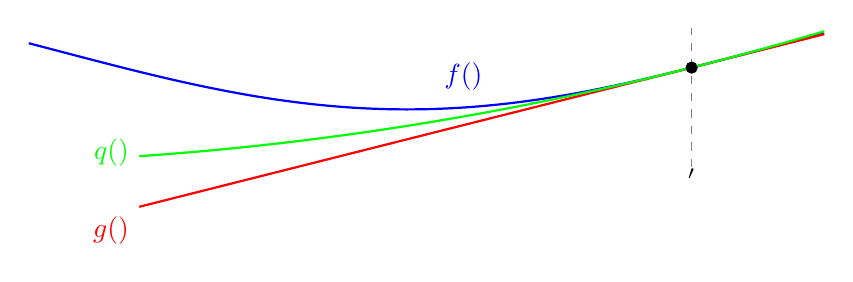
\begin{tikzpicture}[x=0.5cm]
			\begin{axis}[
				hide axis,
				xmin=3, xmax=6,
				ymin=0, ymax=6,
				domain=0:6,
				samples=100,
				width=10cm,
				height=6cm,
				clip=false
				]
			% Original nonlinear function h(x)
				\addplot[blue, thick, domain=3:6.6] {2 + sin(deg(x))} 
				node[pos=0.5, above right, yshift=3pt] {$f(\featurevec)$};
			% Tangent line as local linear approximation at x = 3
			% h(3) = 2 + sin(3), h'(3) = cos(3)
				\addplot[red, thick, domain=3.5:6.6] 
				{2 + sin(deg(6)) + cos(deg(6))*(x - 6)}
				node[pos=0, below left] {$g(\featurevec)$};
                		%%%%%%%%%%%%%%%%%%%%%%%%%%%%%%%%%%%%%%%%%%%%%%%%
                			\addplot[green, thick, domain=3.5:6.6]
                			{2 + sin(deg(6)) + cos(deg(6))*(x - 6) - 0.5*sin(deg(6))*(x - 6)^2}
				node[pos=0, below left, yshift=10pt] {$q(\featurevec)$};
                		%%%%%%%%%%%%%%%%%%%%%%%%%%%%%%%%%%%%%%%%%%%%%%%%
			% Mark point of approximation
				\addplot[mark=*] coordinates {(6, {2 + sin(deg(6))})};
			% Vertical dashed line (ruler) at x = 3
				\addplot[dashed, gray] coordinates {(6,0) (6,2.4)};
				\node at (axis cs:6, -0.2) {$\featurevec'$};
			% Plot the two points
			% Coordinates of the two points
				\pgfmathsetmacro{\xA}{-1.5}
				\pgfmathsetmacro{\xB}{3}
				\pgfmathsetmacro{\yA}{2 + sin(deg(\xA))}
				\pgfmathsetmacro{\yB}{2 + sin(deg(\xB))}
			\end{axis}
			\vspace*{-10mm}
		\end{tikzpicture}
		\vspace*{-5mm}
		\end{center}
		{\selectlanguage{greek}
		\caption{\foreignlanguage{greek}{Μία} \glsentryuseri{function} $f(\featurevec)$ \foreignlanguage{greek}{που είναι επαρκώς} 
			\glsentryuseri{smooth} \foreignlanguage{greek}{σε ένα σημείο $\featurevec'$ μπορεί να προσεγγιστεί τοπικά από μία}
			\glsentryuseriii{quadfunc} $q(\featurevec)$, \foreignlanguage{greek}{η οποία παρέχει μία πιο ορθή προσέγγιση σε σύγκριση
			με μία γραμμική} \glsentryuseriii{function} $g(\featurevec)$. \label{fig_quadapprox_hessian_dict}} }
		\end{figure}
		\foreignlanguage{greek}{Βλέπε επίσης:} \gls{function}, \gls{partialderivative}, \gls{matrix}, \gls{continuous}, \gls{neighborhood}, 
		\gls{symmetricmatrix}, \gls{convex}, \gls{psd}, \gls{quadfunc}, \gls{gradient}, \gls{smooth}. }, 
	first={\foreignlanguage{greek}{Εσσιανός}},
	text={\foreignlanguage{greek}{Εσσιανός}},
	type=math
}

\newglossaryentry{innerproduct}
{name={\foreignlanguage{greek}{εσωτερικό γινόμενο}},
	description={TBC.\index{inner product} },
 	first={\foreignlanguage{greek}{εσωτερικό γινόμενο}},
 	text={\foreignlanguage{greek}{εσωτερικό γινόμενο}},
	type=math,
	user1={\foreignlanguage{greek}{εσωτερικό γινόμενο}}, %nominative
    	user2={\foreignlanguage{greek}{εσωτερικού γινόμενου}}, %genitive
	user3={\foreignlanguage{greek}{εσωτερικό γινόμενο}} %accusative 
}

\newglossaryentry{eucliddist}
{name={\foreignlanguage{greek}{Ευκλείδεια απόσταση}}, 
	description={\foreignlanguage{greek}{Η Ευκλείδεια απόσταση}\index{\foreignlanguage{greek}{Ευκλείδεια απόσταση}} 
		(Euclidean distance) \foreignlanguage{greek}{μεταξύ δύο} \glsentryuserv{vector} $\vw,\vw' \in \mathbb{R}^{\nrfeatures}$
		\foreignlanguage{greek}{είναι η} \glsentryuseri{euclidnorm} \foreignlanguage{greek}{της διαφοράς} $\vw-\vw'$.	
		\\
		\foreignlanguage{greek}{Βλέπε επίσης:} \gls{vector}, \gls{euclidnorm}, \gls{euclidspace}. },
	first={\foreignlanguage{greek}{Ευκλείδεια απόσταση}},
	text={\foreignlanguage{greek}{Ευκλείδεια απόσταση}},
	type=math,
	user1={\foreignlanguage{greek}{Ευκλείδεια απόσταση}}, %nominative
    	user2={\foreignlanguage{greek}{Ευκλείδειας απόστασης}}, %genitive
	user3={\foreignlanguage{greek}{Ευκλείδεια απόσταση}}, %accusative 
	user4={\foreignlanguage{greek}{Ευκλείδειες αποστάσεις}}, %nominativepl
    	user5={\foreignlanguage{greek}{Ευκλείδειων αποστάσεων}}, %genitivepl
	user6={\foreignlanguage{greek}{Ευκλείδειες αποστάσεις}} %accusativepl 
}

\newglossaryentry{euclidnorm}
{name={\foreignlanguage{greek}{Ευκλείδεια νόρμα}}, 
	description={\foreignlanguage{greek}{Η Ευκλείδεια}\index{\foreignlanguage{greek}{Ευκλείδεια νόρμα}}
		\glsentryuseri{norm} (Euclidean norm) $\normgeneric{\weights}{2}$ \foreignlanguage{greek}{ενός} \glsentryuserii{vector} 
		$$\weights = \big(\weight_{1},\,\ldots,\,\weight_{\nrfeatures} \big) \in
		\mathbb{R}^{\nrfeatures}$$
		\foreignlanguage{greek}{ορίζεται ως} 
		$$\normgeneric{\weights}{2} \defeq \sqrt{\sum_{\featureidx=1}^{\nrfeatures}\weight^2_{\featureidx}}.$$ 
		\foreignlanguage{greek}{Η Ευκλείδεια} \glsentryuseri{norm} \foreignlanguage{greek}{είναι διαφορετική από 
		όλες τις} \glsentryuservi{norm} \foreignlanguage{greek}{στον $\mathbb{R}^{\nrfeatures}$, υπό την έννοια ότι 
		επάγεται από το} \glsentryuseriii{innerproduct} $\vw^{T} \vv$ \cite{RudinBook}, \cite{BoydConvexBook}, \cite{HalmosFiniteDimVecSpace}. 
		\foreignlanguage{greek}{Με άλλα λόγια,} $\normgeneric{\weights}{2}= \sqrt{\weights^{T} \weights}$.	
		\\
		\foreignlanguage{greek}{Βλέπε επίσης:} \gls{norm}, \gls{vector}, \gls{innerproduct}, \gls{euclidspace}. },
	first={\foreignlanguage{greek}{Ευκλείδεια νόρμα}},
	text={\foreignlanguage{greek}{Ευκλείδεια νόρμα}},
	type=math,
	user1={\foreignlanguage{greek}{Ευκλείδεια νόρμα}}, %nominative
  	user2={\foreignlanguage{greek}{Ευκλείδειας νόρμας}}, %genitive 
	user3={\foreignlanguage{greek}{Ευκλείδεια νόρμα}} %accusative
}

\newglossaryentry{euclidspace}
{name={\foreignlanguage{greek}{Ευκλείδειος χώρος}}, 
	description={\foreignlanguage{greek}{Ο Ευκλείδειος χώρος}\index{\foreignlanguage{greek}{Ευκλείδειος χώρος}} 
		$\mathbb{R}^{\featuredim}$ \foreignlanguage{greek}{διάστασης $\featuredim \in \mathbb{N}$ αποτελείται 
		από} \glsentryuservi{vector} $\featurevec= \big(\feature_{1}, \,\ldots, \,\feature_{\featurelen}\big)$, 
		\foreignlanguage{greek}{με $\featuredim$ καταχωρίσεις πραγματικής τιμής 
		$\feature_{1}, \,\ldots, \,\feature_{\featuredim} \in \mathbb{R}$. 
		Ένας τέτοιος Ευκλείδειος χώρος είναι εξοπλισμένος με μία γεωμετρική δομή 
		που ορίζεται από το} \glsentryuseriii{innerproduct} 
		$\featurevec\,^{T} \featurevec' = \sum_{\featureidx=1}^{\featuredim} \feature_{\featureidx} \feature'_{\featureidx}$ 
		\foreignlanguage{greek}{μεταξύ οποιωνδήποτε δύο} \glsentryuserv{vector} 
		$\featurevec,\featurevec' \in \mathbb{R}^{\featuredim}$ \cite{RudinBookPrinciplesMatheAnalysis}. 
		\\
		\foreignlanguage{greek}{Βλέπε επίσης:} \gls{vector}, \gls{innerproduct}. },
	first={\foreignlanguage{greek}{Ευκλείδειος χώρος}}, 
	text={\foreignlanguage{greek}{Ευκλείδειος χώρος}},
	type=math,
	user1={\foreignlanguage{greek}{Ευκλείδειος χώρος}}, %nominative
  	user2={\foreignlanguage{greek}{Ευκλείδειου χώρου}}, %genitive 
	user3={\foreignlanguage{greek}{Ευ\-κλεί\-δει\-ο χώρο}}, %accusative 
	user4={\foreignlanguage{greek}{Ευκλείδειοι χώροι}}, %nominativepl
	user5={\foreignlanguage{greek}{Ευκλείδειων χώρων}}, %genitivepl
	user6={\foreignlanguage{greek}{Ευκλείδειους χώρους}}, %accusativepl
}

\newglossaryentry{psd}
{name={\foreignlanguage{greek}{θετικά ημιορισμένος}},
	description={\foreignlanguage{greek}{Ένας} \glsentryuseri{symmetricmatrix}\index{\foreignlanguage{greek}{θετικά ημιορισμένος}} 
		\foreignlanguage{greek}{(πραγματικών τιμών)} $\mQ = \mQ\,^{T} \in \mathbb{R}^{\featuredim \times \featuredim}$ 
		\foreignlanguage{greek}{αναφέρεται ως θετικά ημιορισμένος} (positive semi-definite - psd) \foreignlanguage{greek}{αν 
		$\featurevec\,^{T} \mQ \featurevec \geq 0$ για κάθε} \glsentryuseriii{vector} $\featurevec \in \mathbb{R}^{\featuredim}$. 
		\foreignlanguage{greek}{Ένας θετικά ημιορισμένος} \glsentryuseri{matrix} $\mQ$ \foreignlanguage{greek}{αποδέχεται μία} 
		\glsentryuseriii{spectraldecomp} \foreignlanguage{greek}{με μη αρνητκές} \glsentryuservi{eigenvalue} 
		$\eigval{1}, \,\ldots, \,\eigval{\featuredim} \geq 0$ \cite{HornMatAnalysis}, \cite{Axler2025}. 
		\foreignlanguage{greek}{Η έννοια του να είναι θετικά ημιορισμένος μπορεί να επεκταθεί 
		από} \glsentryuservi{matrix} \foreignlanguage{greek}{σε συμμετρικές} \glsentryuservi{map} \glsentryuserii{kernel} 
		\foreignlanguage{greek}{(πραγματικών τιμών)} $\kernel: \featurespace \times \featurespace \rightarrow \mathbb{R}$ 
		(\foreignlanguage{greek}{με $\kernel(\featurevec,\featurevec') = \kernel(\featurevec',\featurevec)$) ως εξής: Για οποιοδήποτε 
		πεπερασμένο σύνολο} \glsentryuserv{featurevec} $\featurevec^{(1)}, \,\ldots, \,\featurevec^{(\samplesize)}$, \foreignlanguage{greek}{ο 
		επακόλουθος} \glsentryuseri{matrix} $\mQ \in \mathbb{R}^{\samplesize \times \samplesize}$ \foreignlanguage{greek}{με 
		καταχωρίσεις $Q_{\sampleidx,\sampleidx'} = \kernelmap{\featurevec^{(\sampleidx)}}{\featurevec^{(\sampleidx')}}$ 
		είναι θετικά ημιορισμένος} \cite{LearningKernelsBook}.
		\\
		\foreignlanguage{greek}{Βλέπε επίσης:} \gls{symmetricmatrix}, \gls{vector}, \gls{matrix}, \gls{spectraldecomp}, \gls{eigenvalue}, 
		\gls{kernel}, \gls{map}, \gls{featurevec}.},
	first={\foreignlanguage{greek}{θετικά ημιορισμένος}},
	text={\foreignlanguage{greek}{θετικά ημιορισμένος}},
	type=math,
	user1={\foreignlanguage{greek}{θετικά ημιορισμένος}}, %nominative
  	user2={\foreignlanguage{greek}{θετικά ημιορισμένου}}, %genitive 
	user3={\foreignlanguage{greek}{θετικά ημιορισμένο}}, %accusative
	user4={\foreignlanguage{greek}{θετικά ημιορισμένη}} %nominativefem 
}

 \newglossaryentry{singularvalue}
 {name={\foreignlanguage{greek}{ιδιάζουσα τιμή}}, 
 	description={\foreignlanguage{greek}{Βλέπε}\index{\foreignlanguage{greek}{ιδιάζουσα τιμή}} \gls{svd}.},
 	first={\foreignlanguage{greek}{ιδιάζουσα τιμή}},
	text={\foreignlanguage{greek}{ιδιάζουσα τιμή}},
	type=math,
	user1={\foreignlanguage{greek}{ιδιάζουσα τιμή}}, %nominative
  	user2={\foreignlanguage{greek}{ιδιάζουσας τιμής}}, %genitive 
	user3={\foreignlanguage{greek}{ιδιάζουσα τιμή}}, %accusative
	user4={\foreignlanguage{greek}{ιδιάζουσες τιμές}}, %nominativepl
  	user5={\foreignlanguage{greek}{ιδιαζουσών τιμών}}, %genitivepl 
	user6={\foreignlanguage{greek}{ιδιάζουσες τιμές}} %accusativepl
}

\newglossaryentry{eigenvector}
{name={\foreignlanguage{greek}{ιδιοδιάνυσμα}}, 
	description={\foreignlanguage{greek}{Ένα ιδιοδιάνυσμα ενός} \glsentryuserii{matrix}\index{\foreignlanguage{greek}{ιδιοδιάνυσμα}} 
		$\mathbf{A} \in \mathbb{R}^{\featuredim \times \featuredim}$ 
		\foreignlanguage{greek}{είναι ένα μη μηδενικό} \glsentryuseri{vector} $\vx \in \mathbb{R}^{\featuredim} \setminus \{ \mathbf{0} \}$ 
		\foreignlanguage{greek}{τέτοιο ώστε $\mathbf{A} \vx = \lambda \vx$ με κάποια} \glsentryuseriii{eigenvalue} $\lambda$.\\
		\foreignlanguage{greek}{Βλέπε επίσης:} \gls{matrix}, \gls{vector}, \gls{eigenvalue}.},
	first={\foreignlanguage{greek}{ιδιοδιάνυσμα}},
	text={\foreignlanguage{greek}{ιδιοδιάνυσμα}},
	type=math,
	user1={\foreignlanguage{greek}{ιδιοδιάνυσμα}}, %nominative
	user2={\foreignlanguage{greek}{ιδιοδιανύσματος}}, %genitive  
	user3={\foreignlanguage{greek}{ιδιοδιάνυσμα}}, %accusative
	user4={\foreignlanguage{greek}{ιδιοδιανύσματα}}, %nominativepl
	user5={\foreignlanguage{greek}{ιδιοδιανυσμάτων}}, %genitivepl
	user6={\foreignlanguage{greek}{ιδιοδιανύσματα}} %accusativepl
}

\newglossaryentry{markovprop}
{name={\foreignlanguage{greek}{ιδιότητα} Markov},
	description={\foreignlanguage{greek}{Βλέπε} \gls{markovchain}\index{\foreignlanguage{greek}{ιδιότητα} Markov}.},
	first={\foreignlanguage{greek}{ιδιότητα} Markov},
	text={\foreignlanguage{greek}{ιδιότητα} Markov},
	type=math,
	user1={\foreignlanguage{greek}{ιδιότητα} Markov}, %nominative
  	user2={\foreignlanguage{greek}{ιδιότητας} Markov}, %genitive 
	user3={\foreignlanguage{greek}{ιδιότητα} Markov} %accusative
}

\newglossaryentry{eigenvalue}
{name={\foreignlanguage{greek}{ιδιοτιμή}}, 
	description={\foreignlanguage{greek}{Αναφερόμαστε σε έναν αριθμό}\index{\foreignlanguage{greek}{ιδιοτιμή}} 
		$\eigvalgen \in \mathbb{R}$ \foreignlanguage{greek}{ως μία ιδιοτιμή ενός τετραγωνικού} \glsentryuserii{matrix} 
		$\mathbf{A} \in \mathbb{R}^{\featuredim \times \featuredim}$  
		\foreignlanguage{greek}{αν υφίσταται ένα μη μηδενικό} \glsentryuseri{vector} 
		$\vx \in \mathbb{R}^{\featuredim} \setminus \{ \mathbf{0} \}$ \foreignlanguage{greek}{τέτοιο 
		ώστε} $\mathbf{A} \vx = \eigvalgen \vx$ (\foreignlanguage{greek}{βλέπε Σχ.} \ref{fig_eigenvalue_dict}). 
		\begin{figure}[H]
			\centering
			\begin{tikzpicture}[>=stealth, line width=0.8pt]
				% Original vector x
				\draw[->] (0,0) -- (2,1)
				node[midway, above left] {$\vx$};
				% Matrix box A, vertically centered at y = 0.5
				\node[
				minimum width=1.6cm,
				minimum height=1.2cm
				] (A) at (3.0,0.5) {$\mA$};					% Arrow from vector to matrix
				\draw[->] (2,0.5) -- (2.5,0.5);
				% Arrow from matrix to output space
				\draw[->] (3.5,0.5) -- (4.0,0.5);
				% Scaled eigenvector lambda x (collinear with x)
				\draw[->] (4.6,0) -- (5.6,0.5)
				node[midway, above] {$\lambda \vx$};
			\end{tikzpicture}
		{\selectlanguage{greek}
		\caption{\foreignlanguage{greek}{Αυτό το} \glsentryuseri{vector} \foreignlanguage{greek}{είναι το} \glsentryuseri{eigenvector} 
			\foreignlanguage{greek}{που αντιστοιχεί στην ιδιοτιμή} $\eigvalgen$.
			\label{fig_eigenvalue_dict} } }
		\end{figure}
		\foreignlanguage{greek}{Βλέπε επίσης:} \gls{matrix}, \gls{vector}, \gls{eigenvector}. },
	first={\foreignlanguage{greek}{ιδιοτιμή}},
	text={\foreignlanguage{greek}{ιδιοτιμή}},
	type=math,
	user1={\foreignlanguage{greek}{ιδιοτιμή}}, %nominative
	user2={\foreignlanguage{greek}{ιδιοτιμής}}, %genitive  
	user3={\foreignlanguage{greek}{ιδιοτιμή}}, %accusative
	user4={\foreignlanguage{greek}{ιδιοτιμές}}, %nominativepl
	user5={\foreignlanguage{greek}{ιδιοτιμών}}, %genitivepl
	user6={\foreignlanguage{greek}{ιδιοτιμές}} %accusativepl
}

\newglossaryentry{trace}
{name={\foreignlanguage{greek}{ίχνος}},
 	description={TBC.\index{trace} },
    	first={\foreignlanguage{greek}{ίχνος}},
    	text={\foreignlanguage{greek}{ίχνος}},
	type=math,
	user1={\foreignlanguage{greek}{ίχνος}}, %nominative
  	user2={\foreignlanguage{greek}{ίχνους}}, %genitive 
	user3={\foreignlanguage{greek}{ίχνος}} %accusative 
}

\newglossaryentry{normalmatrix}
{name={\foreignlanguage{greek}{κανονικός πίνακας}},
	description={A normal \gls{matrix} is a square \gls{matrix} $\mA \in \mathbb{C}^{\nrfeatures \times \nrfeatures}$ 
                 that commutes with its \gls{conjugatetranspose}, i.e., $\mA\mA^{H}=\mA^{H}\mA$. 
                 Normal \glspl{matrix}\index{normal matrix} admit an orthonormal basis of \glspl{eigenvector} and are 
                 unitarily \gls{diagonalizable}.
                 \\
                 See also: \gls{matrix}, \gls{diagonalizable}. },
	first={\foreignlanguage{greek}{κανονικός πίνακας}},
	text={\foreignlanguage{greek}{κανονικός πίνακας}},
	type=math,
	user1={\foreignlanguage{greek}{κανονικός πίνακας}}, %nominative
	user2={\foreignlanguage{greek}{κανονικού πίνακα}}, %genitive  
	user3={\foreignlanguage{greek}{κανονικό πίνακα}} %accusative 
}

\newglossaryentry{probdist}
{name={\foreignlanguage{greek}{κατανομή πιθανότητας}},
	description={\foreignlanguage{greek}{Για να αναλύσουμε μεθόδους}\index{\foreignlanguage{greek}{κατανομή πιθανότητας}} 
		\glsentryuserii{ml}, \foreignlanguage{greek}{μπορεί να είναι χρήσιμο να ερμηνεύσουμε} \glsentryuservi{datapoint} \foreignlanguage{greek}{ως} 
		\glsentryuseriii{iid} \glsentryuservi{realization} \foreignlanguage{greek}{μίας} \glsentryuserii{rv}. \foreignlanguage{greek}{Οι τυπικές  
		ιδιότητες τέτοιων} \glsentryuserv{datapoint} \foreignlanguage{greek}{διέπονται τότε από την κατανομή} \glsentryuserii{probability}  
		\foreignlanguage{greek}{αυτής της} \glsentryuserii{rv}. \foreignlanguage{greek}{Η κατανομή} \glsentryuserii{probability} 
		\foreignlanguage{greek}{μίας δυαδικής} \glsentryuserii{rv} $\truelabel \in \{0,1\}$ \foreignlanguage{greek}{προσδιορίζεται πλήρως
		από τις πιθανότητες $\prob{\truelabel = 0}$ και 
		$\prob{\truelabel=1}\!=\!1\!-\!\prob{\truelabel=0}$. Η κατανομή} \glsentryuserii{probability} 
		\foreignlanguage{greek}{μίας} \glsentryuserii{rv} \foreignlanguage{greek}{πραγματικής τιμής $\feature \in \mathbb{R}$ μπορεί να 
		προσδιορίζεται από μία} \glsentryuseriii{pdf} $p(\feature)$ \foreignlanguage{greek}{έτσι ώστε $\prob{ \feature \in [a,b] } \approx  p(a) |b-a|$. 
	    	Στην πιο γενική περίπτωση, η κατανομή} \glsentryuserii{probability} \foreignlanguage{greek}{ορίζεται από ένα μέτρο} 
		\glsentryuserii{probability} \cite{BillingsleyProbMeasure}, \cite{GrayProbBook}.\\
	    	\foreignlanguage{greek}{Βλέπε επίσης:} \gls{ml}, \gls{datapoint}, \gls{iid}, \gls{realization}, \gls{rv}, \gls{probability}, \gls{pdf}. },
	 first={\foreignlanguage{greek}{κατανομή πιθανότητας}},
	 text={\foreignlanguage{greek}{κατανομή πιθανότητας}},
	 type=math,
	 user1={\foreignlanguage{greek}{κατανομή πιθανότητας}}, %nominative
	 user2={\foreignlanguage{greek}{κατανομής πιθανότητας}}, %genitive  
	 user3={\foreignlanguage{greek}{κατανομή πιθανότητας}}, %accusative 
	 user4={\foreignlanguage{greek}{κατανομές πιθανοτήτων}}, %nominativepl
	 user5={\foreignlanguage{greek}{κατανομών πιθανοτήτων}}, %genitivepl  
	 user6={\foreignlanguage{greek}{κατανομές πιθανοτήτων}}, %accusativepl 
	 user7={\foreignlanguage{greek}{κατανομής πιθανότητάς}} %genitivedoublestress
}

\newglossaryentry{condprobdist}
{name={\foreignlanguage{greek}{κατανομή πιθανότητας υπό συνθήκη}}, 
	description={\foreignlanguage{greek}{Θεωρούμε μία}\index{\foreignlanguage{greek}{κατανομή πιθανότητας υπό συνθήκη}} 
		\glsentryuseriii{stochproc} \foreignlanguage{greek}{που αποτελείται από δύο} \glsentryuservi{rv} $\featurevec$ 
		\foreignlanguage{greek}{και $\truelabel$ με} \glsentryuseriii{probdist} $\probdist^{(\featurevec,\truelabel)}$. 
		\foreignlanguage{greek}{Η υπό συνθήκη} \glsentryuseri{probdist} \foreignlanguage{greek}{της $\truelabel$ δεδομένης 
		(ή υπό τον όρο) της $\featurevec$ δηλώνεται με $\probdist^{(\truelabel|\featurevec)}$. Ορίζεται μέσω των} 
    		\glsentryuserv{conditionalexpect} \foreignlanguage{greek}{των} \glsentryuserv{function}-\foreignlanguage{greek}{δεικτών}  
    		\glsentryuserv{measurable} \foreignlanguage{greek}{συνόλων στη} \glsentryuseriii{sigmaalgebra} 
		\foreignlanguage{greek}{που παράγεται από την} \glsentryuseriii{rv} $\truelabel$ \cite{BillingsleyProbMeasure}, \cite{KallenbergBook}. \\
		\foreignlanguage{greek}{Βλέπε επίσης:} \gls{stochproc}, \gls{rv}, \gls{probdist}, \gls{conditionalexpect}, 
		\gls{function}, \gls{measurable}, \gls{sigmaalgebra}. },
  	first={\foreignlanguage{greek}{κατανομή πιθανότητας υπό συνθήκη}}, 
  	text={\foreignlanguage{greek}{κατανομή πιθανότητας υπό συνθήκη}},
	type=math,
	user1={\foreignlanguage{greek}{κατανομή πιθανότητας υπό συνθήκη}}, %nominative
  	user2={\foreignlanguage{greek}{κατανομής πιθανότητας υπό συνθήκη}}, %genitive 
	user3={\foreignlanguage{greek}{κατανομή πιθανότητας υπό συνθήκη}} %accusative
}

\newglossaryentry{state}
{name={\foreignlanguage{greek}{κατάσταση}},
	description={\foreignlanguage{greek}{Μία κατάσταση} (state)\index{\foreignlanguage{greek}{κατάσταση}} 
		\foreignlanguage{greek}{είναι μία μαθηματική αναπαράσταση των ελάχιστων πληροφοριών  
		που χρειάζονται για να χαρακτηριστεί ένα σύστημα σε μία δεδομένη στιγμή, έτσι ώστε, 
		μαζί με τη δυναμική του συστήματος, να επαρκούν για την πρόβλεψη 
		της μελλοντικής συμπεριφοράς του συστήματος} \cite{SuttonEd2}, \cite{BertsekasDynOptII}. 	
		\\
		\foreignlanguage{greek}{Βλέπε επίσης:} \gls{featurevec}, \gls{hypothesis}, \gls{action}.},
	first={\foreignlanguage{greek}{κατάσταση}},
	text={\foreignlanguage{greek}{κατάσταση}},
	type=math,
	user1={\foreignlanguage{greek}{κατάσταση}}, %nominative
  	user2={\foreignlanguage{greek}{κατάστασης}}, %genitive 
	user3={\foreignlanguage{greek}{κατάσταση}}, %accusative
	user4={\foreignlanguage{greek}{καταστάσεις}}, %nominativepl
  	user5={\foreignlanguage{greek}{καταστάσεων}}, %genitive pl
	user6={\foreignlanguage{greek}{καταστάσεις}} %accusativepl
}

\newglossaryentry{dag}
{name={\foreignlanguage{greek}{κατευθυνόμενος μη κυκλικός γράφος}},
	description={TBC.\index{directed acyclic graph (DAG)} }, 
 	first={\foreignlanguage{greek}{κατευθυνόμενος μη κυκλικός γράφος}},
 	text={\foreignlanguage{greek}{κατευθυνόμενος μη κυκλικός γράφος}},
	type=math,
	user1={\foreignlanguage{greek}{κατευθυνόμενος μη κυκλικός γράφος}}, %nominative
  	user2={\foreignlanguage{greek}{κατευθυνόμενου μη κυκλικού γράφου}}, %genitive 
	user3={\foreignlanguage{greek}{κατευθυνόμενο μη κυκλικό γράφο}}, %accusative
}

\newglossaryentry{clt}
{name={\foreignlanguage{greek}{κεντρικό οριακό θεώρημα}},
	description={TBC.\index{central limit theorem (CLT)} },
	first={\foreignlanguage{greek}{κεντρικό οριακό θεώρημα}},
	text={\foreignlanguage{greek}{κεντρικό οριακό θεώρημα}},
	type=math, 
	user1={\foreignlanguage{greek}{κεντρικό οριακό θεώρημα}} %nominative
}

\newglossaryentry{gradient}
{name={\foreignlanguage{greek}{κλίση}},
	description={\foreignlanguage{greek}{Για μία}\index{\foreignlanguage{greek}{κλίση}} 
		\glsentryuseriii{function} \foreignlanguage{greek}{πραγματικής τιμής 
		$f: \mathbb{R}^{\featuredim} \rightarrow \mathbb{R}: \weights \mapsto f(\weights)$, 
		αν υφίσταται ένα} \glsentryuseri{vector} $\vg$ \foreignlanguage{greek}{τέτοιο ώστε 
		$$\lim_{\weights \rightarrow \weights'} {f(\weights) - \big(f(\weights') + \vg\,^{T} (\weights - \weights') \big) }/{\| \weights - \weights'\|}=0,$$
		αναφέρεται ως η κλίση} (gradient) \foreignlanguage{greek}{της $f$ στο $\weights'$. Αν υφίσταται, η κλίση είναι μοναδική και 
		δηλώνεται με $\nabla f(\weights')$ ή} $\nabla f(\weights)\big|_{\weights'}$ \cite{RudinBookPrinciplesMatheAnalysis}.
		\foreignlanguage{greek}{Για μία} \glsentryuseriii{differentiable} \glsentryuseriii{function}, \foreignlanguage{greek}{η κλίση είναι το} 
		\glsentryuseri{vector} \foreignlanguage{greek}{του οποίου οι καταχωρίσεις είναι οι} \glsentryuseriv{partialderivative} 
		\foreignlanguage{greek}{της $f$ ως προς κάθε συνιστώσα εισόδου, έτσι ώστε  
		$\nabla f(\weights) = [{\partial f}/{\partial \feature_1}, \,\dots, \,{\partial f}/{\partial \feature_{\featuredim}}]^T$. 
		Γεωμετρικά, η κλίση δείχνει την κατεύθυνση της μέγιστης αύξησης}.
		\\
		\foreignlanguage{greek}{Βλέπε επίσης:} \gls{function}, \gls{vector}, \gls{differentiable}, \gls{partialderivative}, \gls{gdmethod}, \gls{gd}, 
		\gls{zerogradientcondition},  \gls{hessian}. },
	first={\foreignlanguage{greek}{κλίση}},
	text={\foreignlanguage{greek}{κλίση}},
	type=math, 
	user1={\foreignlanguage{greek}{κλίση}}, %nominative
  	user2={\foreignlanguage{greek}{κλίσης}}, %genitive   
	user3={\foreignlanguage{greek}{κλίση}}, %accusative   
	user4={\foreignlanguage{greek}{κλίσεις}}, %nominativepl
  	user5={\foreignlanguage{greek}{κλίσεων}}, %genitivepl   
	user6={\foreignlanguage{greek}{κλίσεις}} %accusativepl 
}

\newglossaryentry{convexopt}
{name={\foreignlanguage{greek}{κυρτή βελτιστοποίηση}},
 	description={TBC.\index{convex optimization} },
	first={\foreignlanguage{greek}{κυρτή βελτιστοποίηση}},
	type=math,
  	text={\foreignlanguage{greek}{κυρτή βελτιστοποίηση}}
}

\newglossaryentry{convex}
{name={\foreignlanguage{greek}{κυρτό}},
	description={\foreignlanguage{greek}{Ένα υποσύνολο}\index{\foreignlanguage{greek}{κυρτός}} 
		$\mathcal{C} \subseteq \mathbb{R}^{\featuredim}$  
		\foreignlanguage{greek}{του} \glsentryuserii{euclidspace} $\mathbb{R}^{\featuredim}$ \foreignlanguage{greek}{αναφέρεται 
		ως κυρτό} (convex) \foreignlanguage{greek}{αν περιέχει το ευθύγραμμο τμήμα μεταξύ οποιωνδήποτε δύο σημεί\-ων 
		$\vx, \vy\!\in\!\cluster$ σε αυτό το σύνολο, δηλαδή}
		$$ \alpha \vx + (1-\alpha) \vy \in \mathcal{C} \quad \mbox{\foreignlanguage{greek}{για κάθε} } \alpha \in [0,1]. $$
		\foreignlanguage{greek}{Όμοια, μία} \glsentryuseri{function} $f\!:\!\mathbb{R}^{\dimlocalmodel}\!\rightarrow\!\mathbb{R}$ 
		\foreignlanguage{greek}{είναι κυρτή αν ο} \glsentryuseri{epigraph} \foreignlanguage{greek}{της} 
		$\big\{ \big( \weights\,^{T},t \big)\,^{T}\!\in\!\mathbb{R}^{\dimlocalmodel\!+\!1}\!:\!t\!\geq\!f(\weights) \}$ 
		\foreignlanguage{greek}{είναι ένα κυρτό σύνολο} \cite{BoydConvexBook}. \foreignlanguage{greek}{Παρουσιάζουμε ένα παράδειγμα 
		ενός κυρτού συνόλου και μίας κυρτής} \glsentryuserii{function} \foreignlanguage{greek}{στο Σχ.} \ref{fig_convex_set_function_dict}. 
		\begin{figure}[H]
		\begin{center}
			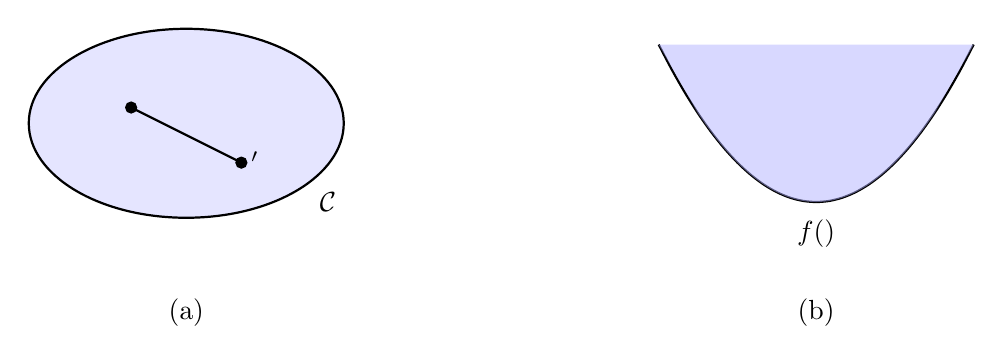
\begin{tikzpicture}
				\fill[blue!20, opacity=0.5] (-3,0) ellipse (2 and 1.2); 
				\draw[thick] (-3,0) ellipse (2 and 1.2);
				\filldraw[black] (-3.7,0.2) circle (2pt) node[left] {$\vw$};
				\filldraw[black] (-2.3,-0.5) circle (2pt) node[right] {$\vw'$};
				\draw[thick] (-3.7,0.2) -- (-2.3,-0.5);
				\node at (-1.2,-1.0) {$\mathcal{C}$};
				\node at (-3,-2.4) {(a)};
				\begin{scope}[shift={(5,-1)}]
					\draw[thick, domain=-2:2, smooth, variable=\x] 
					plot ({\x}, {0.5*\x*\x});
					\fill[blue!30, opacity=0.5] 
					plot[domain=-1.5:1.5, smooth] ({\x}, {0.5*\x*\x}) -- 
					(2, {0.5*2*2}) -- 
					(-2, {0.5*2*2}) -- 
					cycle;
					\node at (0,-0.4) {$f(\weights)$};
					\node at (0,-1.4) {(b)};
				\end{scope}
			\end{tikzpicture}
			\vspace*{-8mm}
			\end{center}
			{\selectlanguage{greek}
			\caption{\selectlanguage{english}{(a)} \foreignlanguage{greek}{Ένα κυρτό σύνολο} 
				$\cluster \subseteq \mathbb{R}^{\dimlocalmodel}$. 
				\selectlanguage{english}{(b)} \foreignlanguage{greek}{Μία κυρτή} \glsentryuseri{function} 
				$f: \mathbb{R}^{\dimlocalmodel} \rightarrow \mathbb{R}$.
				\label{fig_convex_set_function_dict}} }
		\end{figure}
		\foreignlanguage{greek}{Βλέπε επίσης:} \gls{euclidspace}, \gls{function}, \gls{epigraph}.},
	first={\foreignlanguage{greek}{κυρτό}},
	text={\foreignlanguage{greek}{κυρτό}},
	type=math,
	user1={\foreignlanguage{greek}{κυρτό}}, %nominative
	user2={\foreignlanguage{greek}{κυρτού}}, %genitive 
	user3={\foreignlanguage{greek}{κυρτή}}, %nominativeoraccusativefem
	user4={\foreignlanguage{greek}{κυρτής}} %genitivefem
}

\newglossaryentry{smooth}
{name={\foreignlanguage{greek}{λεία}},
	description={TBC.\index{smooth} },
	first={\foreignlanguage{greek}{λεία}},
	text={\foreignlanguage{greek}{λεία}},
	type=math,
	user1={\foreignlanguage{greek}{λεία}}, %nominative
	user2={\foreignlanguage{greek}{λείας}}, %genitive
	user3={\foreignlanguage{greek}{λεία}} %accusative
}

\newglossaryentry{maximum}
{name={\foreignlanguage{greek}{μέγιστο}},
     description={\foreignlanguage{greek}{Το μέγιστο} (maximum) \foreignlanguage{greek}{ενός συνόλου}\index{\foreignlanguage{greek}{μέγιστο}} 
		$\mathcal{A} \subseteq \mathbb{R}$ \foreignlanguage{greek}{πραγματικών αριθμών είναι το μέγιστο στοιχείο σε αυτό το σύνολο, 
		αν ένα τέτοιο στοιχείο υφίσταται. Ένα σύνολο $\mathcal{A}$ έχει ένα μέγιστο αν είναι άνω φραγμένο και 
		επιτυγχάνει το} \glsentryuseriii{supremum} \foreignlanguage{greek}{του} \cite[\foreignlanguage{greek}{Ενότητα}~1.4]{RudinBookPrinciplesMatheAnalysis}.\\
		\foreignlanguage{greek}{Βλέπε επίσης:} \gls{supremum}.},
 	first={\foreignlanguage{greek}{μέγιστο}},
 	text={\foreignlanguage{greek}{μέγιστο}},
	type=math,
 	user1={\foreignlanguage{greek}{μέγιστο}}, %nominative
 	user2={\foreignlanguage{greek}{μέγιστου}}, %genitive 
 	user3={\foreignlanguage{greek}{μέγιστο}}, %accusative 
 	user4={\foreignlanguage{greek}{μέγιστος}}, %nominativeadjmasc
 	user5={\foreignlanguage{greek}{μέγιστη}}, %nominativeoraccusativeadjfem
	user6={\foreignlanguage{greek}{μέγιστης}} %genitiveadjfem
}

\newglossaryentry{optmethod}
{name={\foreignlanguage{greek}{μέθοδος βελτιστοποίησης}},
	description={\foreignlanguage{greek}{Μία μέθοδος} \glsentryuserii{optimization} (optimization method) 
		\foreignlanguage{greek}{είναι ένας}\index{\foreignlanguage{greek}{μέθοδος βελτιστοποίησης}} 
		\glsentryuseri{algorithm} \foreignlanguage{greek}{που διαβάζει μία αναπαράσταση ενός} \glsentryuserii{optproblem} 
		\foreignlanguage{greek}{ως είσοδο και υπολογίζει μία (προσεγγιστική) λύση ως} \glsentryuservii{output}  
		\foreignlanguage{greek}{του. Ένα κεντρικό παράδειγμα} \glsentryuserii{optproblem} \foreignlanguage{greek}{στη} 
		\glsentryuseriii{ml} \foreignlanguage{greek}{είναι η} \glsentryuseri{erm}. \foreignlanguage{greek}{Εφαρμόζοντας μία κατάλληλη
		μέθοδο} \glsentryuserii{optimization} \foreignlanguage{greek}{στην} \glsentryuseriii{erm}, \foreignlanguage{greek}{αποκτούμε έναν 
		συγκεκριμένο} \glsentryuseriii{algorithm} \foreignlanguage{greek}{μάθησης} 
		\cite{BoydConvexBook}, \cite{BertsekasNonLinProgr}, \cite{nesterov04}. 
		\\
		\foreignlanguage{greek}{Βλέπε επίσης:} \gls{optimization}, \gls{algorithm}, \gls{optproblem}, \gls{output}, \gls{ml}, \gls{erm}.},
	first={\foreignlanguage{greek}{μέθοδος βελτιστοποίησης}},
	text={\foreignlanguage{greek}{μέθοδος βελτιστοποίησης}},
	type=math,
	user1={\foreignlanguage{greek}{μέθοδος βελτιστοποίησης}}, %nominative
	user2={\foreignlanguage{greek}{μεθόδου βελτιστοποίησης}}, %genitive  
	user3={\foreignlanguage{greek}{μεθόδο βελτιστοποίησης}} %accusative  
}

\newglossaryentry{admm}
{name={\foreignlanguage{greek}{μέθοδος εναλλασσόμενων διευθύνσεων των πολλαπλασιαστών}},
	description={\foreignlanguage{greek}{Η μέθοδος εναλλασσόμενων διευθύνσεων των 
		πολλαπλασιαστών}\index{\foreignlanguage{greek}{μέθοδος εναλλασσόμενων διευθύνσεων των πολλαπλασιαστών}} 
		(alternating direction method of multipliers - ADMM) \foreignlanguage{greek}{είναι μία επαναληπτική} 
		\glsentryuseri{optmethod} \foreignlanguage{greek}{για τη λύση ενός δομημένου} \glsentryuserii{optproblem}. 
		\foreignlanguage{greek}{Συγκεκριμένα, η μέθοδος εναλλασσόμενων διευθύνσεων των πολλαπλασιαστών 
		μπορεί να χρησιμοποιηθεί για τη λύση ενός} \glsentryuserii{optproblem} \foreignlanguage{greek}{της μορφής} 
		\begin{align}
			\min_{\featurevec \in \mathbb{R}^{\nrfeatures},\featurevec' \in \mathbb{R}^{\nrfeatures'}} \; f(\featurevec) 
			+ g(\featurevec') \nonumber \\ 
			\mbox{ s.t. } \mA \featurevec - \mB \featurevec' = \vc, \nonumber
		\end{align}
		\foreignlanguage{greek}{για δεδομένους} \glsentryuservi{matrix} $\mA \in \mathbb{R}^{p \times \nrfeatures}$ 
		\foreignlanguage{greek}{και} $\mB \in \mathbb{R}^{p \times \nrfeatures'}$,
		\foreignlanguage{greek}{καθώς και ένα δεδομένο} \glsentryuseriii{vector} $\vc \in \mathbb{R}^p$.
		\\
		\foreignlanguage{greek}{Βλέπε επίσης:} \gls{optmethod}, \gls{optproblem}, \gls{matrix}, \gls{vector}, \gls{methodofmultipliers}. }, 
	first={\foreignlanguage{greek}{μέθοδος εναλλασσόμενων διευθύνσεων των πολλαπλασιαστών}},
	text={\foreignlanguage{greek}{μέθοδος εναλλασσόμενων διευθύνσεων των πολλαπλασιαστών}},
	type=math,
	user1={\foreignlanguage{greek}{μέθοδος εναλλασσόμενων διευθύνσεων των πολλαπλασιαστών}}, %nominative
  	user2={\foreignlanguage{greek}{μεθόδου εναλλασσόμενων διευθύνσεων των πολλαπλασιαστών}}, %genitive 
	user3={\foreignlanguage{greek}{μέθοδο εναλλασσόμενων διευθύνσεων των πολλαπλασιαστών}}, %accusative
}%μέθοδος πολλαπλασιαστών εναλλασσόμενης κατεύθυνσης / μέθοδος εναλλασσόμενης κατεύθυνσης των πολλαπλασιαστών

\newglossaryentry{methodofmultipliers}
{name={\foreignlanguage{greek}{μέθοδος των πολλαπλασιαστών}},
	description={\foreignlanguage{greek}{Η μέθοδος των πολλαπλασιαστών}\index{\foreignlanguage{greek}{μέθοδος των πολλαπλασιαστών}} 
		(method of multipliers - MoM) \foreignlanguage{greek}{είναι μία επαναληπτική} \glsentryuseri{optmethod} 
		\foreignlanguage{greek}{για τη λύση ενός περιορισμένου} \glsentryuserii{optproblem} 
		\foreignlanguage{greek}{της μορφής} \cite{DistrOptStatistLearningADMM}
		\begin{align}
			\min_{\vx \in \mathbb{R}^{\nrfeatures}} \; f(\vx) \nonumber \\ 
			\mbox{ s.t. } \mathbf{A}\vx = \vb. \nonumber
		\end{align}
		\foreignlanguage{greek}{Εδώ, $f: \mathbb{R}^{\nrfeatures} \rightarrow \mathbb{R}$ δηλώνει την} 
		\glsentryuseriii{objfunc}, $\mathbf{A} \in \mathbb{R}^{m \times \nrfeatures}$ 
		\foreignlanguage{greek}{είναι ένας δεδομένος} \glsentryuseri{matrix}, \foreignlanguage{greek}{και 
		$\vb \in \mathbb{R}^{m}$ είναι ένα δεδομένο} \glsentryuseri{vector}. \foreignlanguage{greek}{Η μέθοδος των 
		πολλαπλασιαστών βασίζεται στον} \gls{augmentedlagrangian}
		\[L_\rho(\vx,\vy) = f(\vx) + \vy^\top \mathbf{A}\vx
		+ \frac{\rho}{2}\normgeneric{\mathbf{A}\vx - \vb}{2}^{2}
		\]
		\foreignlanguage{greek}{όπου $\vy$ δηλώνει το} \glsentryuseriii{vector} \foreignlanguage{greek}{των 
		πολλαπλασιαστών του} Lagrange \foreignlanguage{greek}{και $\rho>0$ είναι μία}
		\glsentryuseri{parameter} \foreignlanguage{greek}{ποινής}. \foreignlanguage{greek}{Η μέθοδος 
		των πολλαπλασιαστών κατασκευάζει μία} \glsentryuseriii{sequence} \foreignlanguage{greek}{εκτιμήσεων 
		$\pair{\vx^{(1)}}{\vy^{(1)}},\,\ldots$ που συγκλίνει σε μία λύση του} \glsentryuserii{optproblem}. 
		\foreignlanguage{greek}{Συγκεκριμένα, κατά τη διάρκεια κάθε} \glsentryuserii{iteration} $\iteridx$, 
		\foreignlanguage{greek}{οι τρέχουσες εκτιμήσεις $\vx^{(\itercntr)},\vy^{(\itercntr)}$
		ενημερώνονται ως εξής:}
		\begin{align*} 
			\vx^{(\itercntr+1)} &= \argmin_{\vx \in \mathbb{R}^{\nrfeatures}} L_\rho(\vx,\vy^{(\itercntr)}) \\
			\vy^{(\itercntr+1)} &= \vy^{(\itercntr)} + \rho\, \big(\mathbf{A}\vx^{(\itercntr+1)} - \vb\big).
		\end{align*}
		\foreignlanguage{greek}{Η μέθοδος των πολλαπλασιαστών μπορεί να γραφεί ως μία} 
		\glsentryuseri{fixedpointiter} \foreignlanguage{greek}{της μορφής} 
		\[
		\big( \vx^{(\itercntr+1)},\vy^{(\itercntr+1)} \big) = \fixedpointop \big(\vx^{(\itercntr)},\vy^{(\itercntr)} \big)
		\]
		\foreignlanguage{greek}{με} 
		\begin{align} 
			\fixedpointop:\mathbb{R}^{\nrfeatures}\!\times\!\mathbb{R}^{m}\!\to\!
			\mathbb{R}^{\nrfeatures}\!\times\!\mathbb{R}^{m}\!:\!\big(\vx,\vy\big)\!&\mapsto\!\big(\vx',\vy\!+\!\rho \big(\mathbf{A}\vx'\!-\!\vb\big) \big) \nonumber \\ 
			& \mbox{ \foreignlanguage{greek}{με} } \vx' = \argmin_{\vx \in \mathbb{R}^{\nrfeatures}} L_\rho(\vx,\vy). \nonumber
		\end{align}
		\foreignlanguage{greek}{Βλέπε επίσης:} \gls{optmethod}, \gls{optproblem}, \gls{objfunc}, \gls{matrix}, \gls{vector}, 
		\gls{augmentedlagrangian}, \gls{parameter}, \gls{sequence}, \gls{iteration}, \gls{fixedpointiter}. }, 
 	first={\foreignlanguage{greek}{μέθοδος των πολλαπλασιαστών}},
 	text={\foreignlanguage{greek}{μέθοδος των πολλαπλασιαστών}},
	type=math,
	user1={\foreignlanguage{greek}{μέθοδος των πολλαπλασιαστών}}, %nominative
  	user2={\foreignlanguage{greek}{μεθόδου των πολλαπλασιαστών}}, %genitive 
	user3={\foreignlanguage{greek}{μέθοδο των πολλαπλασιαστών}}, %accusative
}

\newglossaryentry{partialderivative}
{name={\foreignlanguage{greek}{μερική παράγωγος}},
	description={TBC.\index{partial derivative} },
    	first={\foreignlanguage{greek}{μερική παράγωγος}},
	text={\foreignlanguage{greek}{μερική παράγωγος}},
	type=math, 
	user1={\foreignlanguage{greek}{μερική παράγωγος}}, %nominative
  	user2={\foreignlanguage{greek}{μερικής παραγώγου}}, %genitive 
	user3={\foreignlanguage{greek}{μερική παράγωγο}}, %accusative
	user4={\foreignlanguage{greek}{μερικές παράγωγοι}}, %nominativepl
  	user5={\foreignlanguage{greek}{μερικών παραγώγων}}, %genitivepl 
	user6={\foreignlanguage{greek}{μερικές παραγώγους}} %accusativepl
}

\newglossaryentry{mean}
{name={\foreignlanguage{greek}{μέση τιμή}},
	description={\foreignlanguage{greek}{Η μέση τιμή μίας}\index{\foreignlanguage{greek}{μέση τιμή}} 
		\glsentryuserii{rv} $\featurevec$, \foreignlanguage{greek}{που παίρνει τιμές σε έναν} \glsentryuseriii{euclidspace} $\mathbb{R}^{\dimlocalmodel}$, 
		\foreignlanguage{greek}{είναι η} \glsentryuseri{expectation} \foreignlanguage{greek}{της}
 		$\expect\{\featurevec\}$. \foreignlanguage{greek}{Ορίζεται ως το ολοκλήρωμα} Lebesgue \foreignlanguage{greek}{του} $\featurevec$ 
		\foreignlanguage{greek}{αναφορικά με την υποκείμενη} \glsentryuseriii{probdist} $P$ (\foreignlanguage{greek}{π.χ. βλέπε} 
		\cite{RudinBookPrinciplesMatheAnalysis} \foreignlanguage{greek}{ή} \cite{BillingsleyProbMeasure}), \foreignlanguage{greek}{δηλαδή}
		\[
			\expect\{\featurevec\} = \int_{\mathbb{R}^{\dimlocalmodel}} \vx \, \mathrm{d}P(\vx).
		\] 
		\foreignlanguage{greek}{Είναι χρήσιμο να σκεφτούμε τη μέση τιμή ως τη λύση του ακόλουθου προβλήματος 
		ελαχιστοποίησης} \glsentryuserii{risk} \cite{BertsekasProb}:
		\[
			\expect\{\featurevec\} = \argmin_{\vc \in \mathbb{R}^{\nrfeatures}} 
			\expect \big\{\normgeneric{\featurevec - \vc}{2}^{2}\big \}.
		\] 
		\foreignlanguage{greek}{Χρησιμοποιούμε επίσης τον όρο για να αναφερθούμε στον μέσο όρο μίας πεπερασμένης ακολουθίας  
		$\vx^{(1)}, \,\ldots, \,\vx^{(\samplesize)} \in \mathbb{R}^{\dimlocalmodel}$. Ωστόσο, 
		αυτοί οι δύο ορισμοί είναι ουσιαστικά ίδιοι. Πράγματι, μπορούμε να χρησιμοποιήσουμε την ακολουθία  
		$\vx^{(1)}, \,\ldots, \,\vx^{(\samplesize)} \in \mathbb{R}^{\dimlocalmodel}$ για να κατασκευάσουμε μία διακριτή} \glsentryuseriii{rv} $\widetilde{\vx}=\vx^{(I)}$, 
		\foreignlanguage{greek}{με τον δείκτη $I$ να επιλέγεται ομοιόμορφα στην τύχη από το σύνολο 
		$\{1, \,\ldots, \,\samplesize\}$. Η μέση τιμή της $\widetilde{\vx}$ είναι ακριβώς ο μέσος όρος}
		$({1}/{\samplesize}) \sum_{\sampleidx=1}^{\samplesize} \vx^{(\sampleidx)}$.\\
		\foreignlanguage{greek}{Βλέπε επίσης:} \gls{rv}, \gls{euclidspace}, \gls{expectation}, \gls{probdist}, \gls{risk}.}, 
	first={\foreignlanguage{greek}{μέση τιμή}}, 
	text={\foreignlanguage{greek}{μέση τιμή}},
	type=math,
	user1={\foreignlanguage{greek}{μέση τιμή}}, %nominative
   	user2={\foreignlanguage{greek}{μέσης τιμής}}, %genitive 
	user3={\foreignlanguage{greek}{μέση τιμή}}, %accusative
	user4={\foreignlanguage{greek}{μέσες τιμές}}, %nominativepl
   	user5={\foreignlanguage{greek}{μέσων τιμών}}, %genitivepl 
	user6={\foreignlanguage{greek}{μέσες τιμές}} %accusativepl
}

\newglossaryentry{averagenodedegree}
{name={\foreignlanguage{greek}{μέσος βαθμός κόμβου}},
	description={The average \gls{nodedegree}\index{average node degree} $\avgnodedegree$ of a weighted 
		\gls{undirectedgraph} $\graph=(\nodes,\edges,\mA)$ is the average of 
		all \glspl{nodedegree}, i.e., $\avgnodedegree = (1/\nrnodes) \sum_{\nodeidx \in \nodes} \nodedegree{\nodeidx}$.
					\\ 
		See also: \gls{nodedegree}, \gls{undirectedgraph}, \gls{neighbor}.},
	first={\foreignlanguage{greek}{μέσος βαθμός κόμβου}},
	text={\foreignlanguage{greek}{μέσος βαθμός κόμβου}},
	type=math,
	user1={\foreignlanguage{greek}{μέσος βαθμός κόμβου}}, %nominative
  	user2={\foreignlanguage{greek}{μέσου βαθμού κόμβου}}, %genitive 
	user3={\foreignlanguage{greek}{μέσο βαθμό κόμβου}}, %accusative
}

\newglossaryentry{measurable}
{name={\foreignlanguage{greek}{μετρήσιμο}}, 
	description={\foreignlanguage{greek}{Θεωρούμε ένα}\index{\foreignlanguage{greek}{μετρήσιμο}} \glsentryuseriii{randomexperiment}, 
		\foreignlanguage{greek}{όπως την καταγραφή της θερμοκρασίας του αέρα σε ένα σταθμό καιρού του} 
		\glsentryuserii{fmi}. \foreignlanguage{greek}{Ο αντίστοιχος} \glsentryuseri{samplespace} $\samplespace$ 
		\foreignlanguage{greek}{αποτελείται από όλες τις πιθανές} \glsentryuservi{outcome} $\outcome$ \foreignlanguage{greek}{(π.χ.
		όλες τις πιθανές τιμές θερμοκρασίας σε βαθμούς Κελσίου). Σε πολλές εφαρμογές} \glsentryuserii{ml},
		\foreignlanguage{greek}{δε μας ενδιαφέρει η ακριβής} \glsentryuseriii{outcome} $\outcome$, \foreignlanguage{greek}{αλλά 
		μόνο το αν ανήκει σε ένα υποσύνολο $\mathcal{A} \subseteq \samplespace$ (π.χ. ο καθορισμός του αν η θερμοκρασία 
		είναι κάτω από το μηδέν). Ονομάζουμε ένα τέτοιο υποσύνολο $\mathcal{A}$ μετρήσιμο} (measurable) \foreignlanguage{greek}{αν 
		είναι δυνατό να αποφασίσουμε, για οποιαδήποτε} \glsentryuseriii{outcome} $\outcome$, \foreignlanguage{greek}{αν 
		$\outcome \in \mathcal{A}$ (βλέπε Σχ.}\ \ref{fig_measurable_dict}). \\
		\begin{figure}[H]
		\begin{center}
		\begin{tikzpicture}
			% Draw temperature axis
			\draw[->] (0,0) -- (8.5,0) node[right] {\foreignlanguage{greek}{θερμοκρασία} ($^\circ$C)};
			% Add tick marks and labels every 20 degrees from -20 to 100
			\foreach \x/\label in {0/--20, 1/--10, 2/0, 3/10, 4/20, 5/30, 6/40, 7/50, 8/60} {
			\draw (\x,0.1) -- (\x,-0.1);
			\node[below] at (\x,-0.1) {\label};
			}
			% Shade measurable set: Temperature < 0°C
			\fill[blue!20] (0,0.3) rectangle (2,0.6);
			\node[above] at (1,0.6) {$\outcome < 0\;^\circ$C};
			% Shade measurable set: 5°C < omega < 10°C
			\fill[red!20] (5.5,0.3) rectangle (7.5,0.6);
			\node[above] at (6,0.6) {$35\;^\circ$C $< \outcome < 55\;^\circ$C};
			\vspace*{10mm}
			\end{tikzpicture}
			\vspace*{10mm}
			\end{center}
		{\selectlanguage{greek}
		\caption{\foreignlanguage{greek}{Ένας} \glsentryuseri{samplespace} \foreignlanguage{greek}{που αποτελείται από όλες τις 
			πιθανές τιμές θερμοκρασίας $\outcome$ που μπορούν να εμφανιστούν σε έναν σταθμό του} \glsentryuserii{fmi}. 
			\foreignlanguage{greek}{Δύο μετρήσιμα υποσύνολα τιμών θερμοκρασίας, τα οποία συμβολίζονται με 
			$\mathcal{A}^{(1)}$ και $\mathcal{A}^{(2)}$, επισημαίνονται. Για οποιαδήποτε πραγματική τιμή θερμοκρασίας  
			$\outcome$, είναι δυνατό να καθοριστεί (μέσω κάποιου εξοπλισμού) αν 
			$\outcome \in \mathcal{A}^{(1)}$ και αν} $\outcome \in \mathcal{A}^{(2)}$. 
			\label{fig_measurable_dict}} }
		\end{figure}
		\foreignlanguage{greek}{Στη θεωρία, μετρήσιμα σύνολα μπορούν να επιλεγούν ελεύθερα (π.χ. ανάλογα με την ανάλυση 
		του εξοπλισμού μέτρησης). Ωστόσο, είναι συχνά χρήσιμο να επιβάλλονται ορισμένες απαιτήσεις πληρότητας στη συλλογή 
		των μετρήσιμων συνόλων. Για παράδειγμα, ο ίδιος ο} \glsentryuseri{samplespace} \foreignlanguage{greek}{θα πρέπει να είναι 
		μετρήσιμος, και η ένωση δύο μετρήσιμων συνόλων θα πρέπει επίσης να είναι μετρήσιμη. Αυτές οι απαιτήσεις πληρότητας
		μπορούν να τυποποιηθούν μέσω της έννοιας της} \glsentryuserii{sigmaalgebra} (\foreignlanguage{greek}{ή} \gls{sigmafield}) 
		\cite{RudinBook}, \cite{BillingsleyProbMeasure}, \cite{durrett2010probability}. 
		\foreignlanguage{greek}{Ένας μετρήσιμος χώρος είναι ένα ζεύγος $\big(\featurespace,\eventspace\big)$ που αποτελείται από ένα 
		αυθαίρετο σύνολο $\featurespace$ και μία συλλογή $\eventspace$ μετρήσιμων υποσυνόλων του $\featurespace$ 
		που σχηματίζουν μία} \glsentryuseriii{sigmaalgebra}. 
		\\
		\foreignlanguage{greek}{Βλέπε επίσης:} \gls{randomexperiment}, \gls{fmi}, \gls{samplespace}, \gls{outcome}, \gls{ml}, 
		\gls{sigmaalgebra}, \gls{sigmafield}, \gls{probability}.},
	first={\foreignlanguage{greek}{μετρήσιμο}},
	text={\foreignlanguage{greek}{μετρήσιμο}},
	type=math,
	user1={\foreignlanguage{greek}{μετρήσιμο}}, %nominative
  	user2={\foreignlanguage{greek}{μετρήσιμου}}, %genitive  
	user3={\foreignlanguage{greek}{μετρήσιμο}}, %accusativeormasc
	user4={\foreignlanguage{greek}{μετρήσιμα}}, %nominativepl
  	user5={\foreignlanguage{greek}{μετρήσιμων}}, %genitiveplforall
	user6={\foreignlanguage{greek}{μετρήσιμα}}, %accusativepl
	user7={\foreignlanguage{greek}{μετρήσιμη}}, %nominatieoraccusativefem
	user8={\foreignlanguage{greek}{μετρήσιμες}} %nominatieoraccusativeplfem
}

\newglossaryentry{metric}
{name={\foreignlanguage{greek}{μετρική}},
	description={\foreignlanguage{greek}{Μία μετρική}\index{\foreignlanguage{greek}{μετρική}} (metric)
		\foreignlanguage{greek}{είναι ένα ποσοτικό} \glsentryuseri{measure} \foreignlanguage{greek}{που χρησιμοποιείται 
		για τη σύγκριση αντικειμένων. Στα μαθηματικά, μία μετρική μετράει την απόσταση μεταξύ δύο σημείων 
		σε έναν χώρο και πρέπει να ακολουθεί συγκεκριμένους κανόνες, δηλαδή η απόσταση να είναι πάντα μη αρνητική, 
		να είναι μηδενική μόνο αν τα σημεία είναι ίδια, να είναι συμμετρική, και να ικανοποιεί την τριγωνική ανισότητα}
		\cite{RudinBookPrinciplesMatheAnalysis}. 
		\foreignlanguage{greek}{Στο πλαίσιο της} \glsentryuserii{ml}, \foreignlanguage{greek}{ο όρος μετρική αναφέρεται 
		σε ένα ποσοτικό} \glsentryuseri{measure} \foreignlanguage{greek}{του πόσο καλά επιδίδει ένα} \glsentryuseri{model} 
		\foreignlanguage{greek}{(κάπως όμοιο με μία} \glsentryuseriii{lossfunc}). \foreignlanguage{greek}{Παραδείγματα περιλαμβάνουν 
		την} \glsentryuseriii{acc}, \foreignlanguage{greek}{την} \glsentryuseriii{precision}, \foreignlanguage{greek}{και τη μέση} 
		\glsentryuseriii{zerooneloss} \foreignlanguage{greek}{σε ένα} \glsentryuseriii{testset} \cite{Goodfellow-et-al-2016}, \cite{BishopBook}. 
		\foreignlanguage{greek}{Ο όρος} \glsentryuseri{lossfunc} \foreignlanguage{greek}{χρησιμοποι\-εί\-ται συνήθως στο 
		πλαίσιο της} \glsentryuserii{training} \glsentryuserii{model}, \foreignlanguage{greek}{ενώ ο όρος μετρική χρησιμοποιείται 
		στο πλαίσιο της} \glsentryuserii{validation} \glsentryuserii{model}.
		\\ 
		\foreignlanguage{greek}{Βλέπε επίσης:} \gls{measure}, \gls{ml}, \gls{model}, \gls{lossfunc}, \gls{acc}, \gls{precision}, 
		\gls{zerooneloss}, \gls{testset}, \gls{training}, \gls{validation}, \gls{loss}. },
	first={\foreignlanguage{greek}{μετρική}}, 
	text={\foreignlanguage{greek}{μετρική}},
	type=math,
	user1={\foreignlanguage{greek}{μετρική}}, %nominative
	user2={\foreignlanguage{greek}{μετρικής}}, %genitive  
	user3={\foreignlanguage{greek}{μετρική}}, %accusative
	user4={\foreignlanguage{greek}{μετρικές}}, %nominativepl
	user5={\foreignlanguage{greek}{μετρικών}}, %genitiveplandforadj
	user6={\foreignlanguage{greek}{μετρικές}}, %accusativepl
	user7={\foreignlanguage{greek}{μετρικός}}, %nominativeadjmasc
	user8={\foreignlanguage{greek}{μετρικού}} %genitiveadjmasc
}

\newglossaryentry{metricspace}
{name={\foreignlanguage{greek}{μετρικός χώρος}},
	description={\foreignlanguage{greek}{Ένας} \glsentryuservii{metric}\index{\foreignlanguage{greek}{μετρικός χώρος}} 
		\foreignlanguage{greek}{χώρος} (metric space) \foreignlanguage{greek}{είναι ένα σύνολο $\featurespace$ 
		εξοπλισμένο με μία} \glsentryuseriii{function} (\foreignlanguage{greek}{που αναφέρεται ως μία} 
		\glsentryuseri{metric}) $\metric{\cdot}{\cdot}: \featurespace \times \featurespace \rightarrow \mathbb{R}_{+}$,
		\foreignlanguage{greek}{η οποία ικανοποιεί τις ακόλουθες απαιτήσεις για όλα τα} 
		$\featurevec, \featurevec', \featurevec'' \in \featurespace$:
        		\begin{enumerate}[label=\arabic*)]
            		\item \foreignlanguage{greek}{Μη αρνητικότητα: $\metric{\featurevec}{\featurevec'} \ge 0$·}
           		\item \foreignlanguage{greek}{Ταυτότητα: $\metric{\featurevec}{\featurevec'} = 0$ 
                  		αν και μόνο αν $\featurevec = \featurevec'$·}
            		\item \foreignlanguage{greek}{Συμμετρία: $\metric{\featurevec}{\featurevec'} 
                  		= \metric{\featurevec'}{\featurevec}$·}
            		\item \foreignlanguage{greek}{Τριγωνική ανισότητα}: 
                  		$\metric{\featurevec}{\featurevec''} \le 
                  		\metric{\featurevec}{\featurevec'} + \metric{\featurevec'}{\featurevec''}$.
        		\end{enumerate}
        		\foreignlanguage{greek}{Τυπικά, ένας} \glsentryuservii{metric} \foreignlanguage{greek}{χώρος είναι ένα
		ζεύγος $(\featurespace, \metric{\cdot}{\cdot})$ που ικανοποιεί τις παραπάνω απαιτήσεις.} 
		\begin{figure}[H]
		\centering
		\begin{tikzpicture}[>=stealth, x=0.5cm, y=1cm]
		% --------- Titles ----------
		\node[font=\footnotesize] at (2.5,3.6) {\glsentryuseri{euclidspace} $\mathbb{R}^2$};
		\node[font=\footnotesize] at (12.5,3.6) {\glsentryuseri{undirectedgraph} $\pair{\nodes}{\edges}$};
		% ===== Left panel: Euclidean space =====
		\begin{scope}[shift={(0,0)}]
			% Axes
			\draw[->] (0,0) -- (5.2,0) node[below right] {$\feature_1$};
			\draw[->] (0,0) -- (0,3.2) node[left] {$\feature_2$};
			% Two points x and y
			\coordinate (X) at (1.1,0.9);
			\coordinate (Y) at (3.8,2.1);
			\fill (X) circle (1.2pt) node[below left] {$\featurevec$};
			\fill (Y) circle (1.2pt) node[above right] {$\featurevec'$};
			% Euclidean distance segment with label
			\draw[dashed] (X) -- (Y)
			node[midway, below right, xshift=1pt] {$\normgeneric{\featurevec-\featurevec'}{2}$};
			\node at (3, -1) {(a)};
		\end{scope}
		% ===== Right panel: Undirected graph =====
		\begin{scope}[shift={(9.0,0)}]
			% Nodes
			\coordinate (A) at (1.0,0.6);
			\coordinate (B) at (3.1,0.9);
			\coordinate (C) at (2.2,2.6);
			\coordinate (D) at (4.8,2.2);
			\coordinate (E) at (0.4,2.1);
			% Edges (undirected)
			\draw (A)--(B)--(C)--(E)--(A);
			\draw (C)--(D)--(B);
			% Highlight two nodes i (source) and j (target) and a shortest path
			\fill (A) circle (1.2pt) node[below left] {$\nodeidx$};
			\fill (D) circle (1.2pt) node[above right] {$\nodeidx'$};
			% One shortest path i -- B -- j (length 2)
			\draw[very thick] (A)--(B)--(D);
			\node[font=\footnotesize, above] at (5.0,0.7) {$\metric{\nodeidx}{\nodeidx'}\!=\!2$};
			% Other nodes
			\fill (B) circle (1.2pt);
			\fill (C) circle (1.2pt);
			\fill (E) circle (1.2pt);
			\node at (3, -1) {(b)};
		\end{scope}
		\end{tikzpicture}
		{\selectlanguage{greek}
		\caption{\foreignlanguage{greek}{Παραδείγματα} \glsentryuserv{metric} \foreignlanguage{greek}{χώρων}. 
			\selectlanguage{english}{(a)} \glsentryuseri{euclidspace} $\mathbb{R}^2$ \foreignlanguage{greek}{με την} 
			\glsentryuseriii{eucliddist} \foreignlanguage{greek}{ως μία} \glsentryuseriii{metric}. \selectlanguage{english}{(b)} 
			\glsentryuservii{undirectedgraph} $\pair{\nodes}{\edges}$ \foreignlanguage{greek}{με την απόσταση
			της συντομότερης διαδρομής ως μία} \glsentryuseriii{metric}.\label{fig:metric_space_examples_dict}} }
	    	\end{figure}
		\foreignlanguage{greek}{Ένα περίφημο παράδειγμα} \glsentryuserviii{metric} \foreignlanguage{greek}{χώρου 
		είναι ο} \glsentryuseri{euclidspace} \foreignlanguage{greek}{εξοπλισμένος με μία} \glsentryuseriii{metric} 
		\foreignlanguage{greek}{που δίνεται από την} \glsentryuseriii{eucliddist} 
		$\metric{\featurevec}{\featurevec'} = \normgeneric{\featurevec - \featurevec'}{2}$. 
		\foreignlanguage{greek}{Ένα άλλο καλά γνωστό παράδειγμα} \glsentryuserviii{metric} \foreignlanguage{greek}{χώρου 
		είναι ένας} \glsentryuseri{undirectedgraph}  
		$\graph=\pair{\nodes}{\edges}$, \foreignlanguage{greek}{με τη} \glsentryuseriii{metric} $\metric{\nodeidx}{\nodeidx'}$ 
		\foreignlanguage{greek}{ορισμένη από το μήκος της συντομότερης διαδρομής που συνδέει τους κόμβους 
		$\nodeidx$ και} $\nodeidx'$. 
			\\
		\foreignlanguage{greek}{Βλέπε επίσης:} \gls{metric}, \gls{function}, \gls{euclidspace}, \gls{undirectedgraph}, 
		\gls{eucliddist}, \gls{featurespace}. },
    	text={\foreignlanguage{greek}{μετρικός χώρος}}, 
	first={\foreignlanguage{greek}{μετρικός χώρος}}, 
	type=math,
	user1={\foreignlanguage{greek}{μετρικός χώρος}}, %nominative
	user2={\foreignlanguage{greek}{μετρικού χώρου}}, %genitive  
	user3={\foreignlanguage{greek}{μετρικό χώρο}}, %accusative
	user4={\foreignlanguage{greek}{μετρικοί χώροι}}, %nominativepl
	user5={\foreignlanguage{greek}{μετρικών χώρων}}, %genitivepl  
	user6={\foreignlanguage{greek}{μετρικούς χώρους}} %accusativepl
}

\newglossaryentry{measure}
{name={\foreignlanguage{greek}{μέτρο}},
	description={TBC.\index{measure} },
	first={\foreignlanguage{greek}{μέτρο}},
	text={\foreignlanguage{greek}{μέτρο}},
	type=math,
	user1={\foreignlanguage{greek}{μέτρο}}, %nominative
  	user2={\foreignlanguage{greek}{μέτρου}}, %genitive 
	user3={\foreignlanguage{greek}{μέτρο}}, %accusative
	user4={\foreignlanguage{greek}{μέτρα}}, %nominativepl
  	user5={\foreignlanguage{greek}{μέτρων}}, %genitivepl 
	user6={\foreignlanguage{greek}{μέτρα}} %accusativepl
}

\newglossaryentry{undirectedgraph}
{name={\foreignlanguage{greek}{μη κατευθυνόμενος γράφος}},
	description={\foreignlanguage{greek}{Βλέπε}\index{\foreignlanguage{greek}{μη κατευθυνόμενος γράφος}} \gls{graph}. },
	first={\foreignlanguage{greek}{μη κατευθυνόμενος γράφος}},
	text={\foreignlanguage{greek}{μη κατευθυνόμενος γράφος}},
	type=math,
	user1={\foreignlanguage{greek}{μη κατευθυνόμενος γράφος}}, %nominative
  	user2={\foreignlanguage{greek}{μη κατευθυνόμενου γράφου}}, %genitive 
	user3={\foreignlanguage{greek}{μη κατευθυνόμενο γράφο}}, %accusative
	user4={\foreignlanguage{greek}{μη κατευθυνόμενοι γράφοι}}, %nominativepl
  	user5={\foreignlanguage{greek}{μη κατευθυνόμενων γράφων}}, %genitivepl 
	user6={\foreignlanguage{greek}{μη κατευθυνόμενους γράφους}}, %accusativepl
	user7={\foreignlanguage{greek}{Μη κατευθυνόμενος γράφος}} %nominativecapital
}

\newglossaryentry{nonsmooth}
{name={\foreignlanguage{greek}{μη λεία}},
	description={\foreignlanguage{greek}{Αναφερόμαστε σε μία}\index{\foreignlanguage{greek}{μη λεία}} 
		\glsentryuseriii{function} \foreignlanguage{greek}{ως μη λεία αν δεν είναι} \glsentryuseri{smooth} \cite{nesterov04}.\\
		\foreignlanguage{greek}{Βλέπε επίσης:} \gls{function}, \gls{smooth}.},
	first={\foreignlanguage{greek}{μη λεία}},
	text={\foreignlanguage{greek}{μη λεία}},
	type=math,
	user1={\foreignlanguage{greek}{μη λεία}}, %nominative
	user2={\foreignlanguage{greek}{μη λείας}} %genitive
}

\newglossaryentry{lln}
{name={\foreignlanguage{greek}{νόμος των μεγάλων αριθμών}},
	description={\foreignlanguage{greek}{Ο νόμος των μεγάλων αριθ\-μών}\index{\foreignlanguage{greek}{νόμος των μεγάλων αριθμών}} 
		\foreignlanguage{greek}{αναφέρεται στη} \glsentryuseriii{convergence} \foreignlanguage{greek}{του μέσου όρου ενός αυξανόμενου 
		(μεγάλου) αριθ\-μού} \glsentryuserii{iid} \glsentryuserv{rv} \foreignlanguage{greek}{στη} \glsentryuseriii{mean} \foreignlanguage{greek}{της 
		κοινής τους} \glsentryuserii{probdist}. \foreignlanguage{greek}{Διαφορετικές περιπτώσεις του νόμου των μεγάλων αριθμών 
		προκύπτουν από τη χρήση διαφορετικών εννοιών} \glsentryuserii{convergence} \cite{papoulis}.\\
		\foreignlanguage{greek}{Βλέπε επίσης:} \gls{convergence}, \gls{iid}, \gls{rv}, \gls{mean}, \gls{probdist}.},
	first={\foreignlanguage{greek}{νόμος των μεγάλων αριθμών}},
	text={\foreignlanguage{greek}{νόμος των μεγάλων αριθμών}},
	type=math,
	user1={\foreignlanguage{greek}{νόμος των μεγάλων αριθμών}}, %nominative
	user2={\foreignlanguage{greek}{νόμου των μεγάλων αριθμών}} %genitive
}

\newglossaryentry{norm}
{name={\foreignlanguage{greek}{νόρμα}},
	description={\foreignlanguage{greek}{Μία νόρμα είναι μία}\index{\foreignlanguage{greek}{νόρμα}} \glsentryuseri{function} 
		\foreignlanguage{greek}{που αντιστοιχίζει κάθε} (\glsentryuservii{vector}) \foreignlanguage{greek}{στοιχείο ενός} 
		\glsentryuserii{vectorspace} \foreignlanguage{greek}{σε έναν μη αρνητικό αριθμό. Αυτή η} \glsentryuseri{function} 
		\foreignlanguage{greek}{πρέπει να είναι ομογενής και ορισμένη, και πρέπει να ικανοποιεί την τριγωνική 
		ανισότητα} \cite{HornMatAnalysis}.\\
		\foreignlanguage{greek}{Βλέπε επίσης:} \gls{function}, \gls{vector}, \gls{vectorspace}. },
	first={\foreignlanguage{greek}{νόρμα}},
	text={\foreignlanguage{greek}{νόρμα}},
	type=math,
	user1={\foreignlanguage{greek}{νόρμα}}, %nominative
    	user2={\foreignlanguage{greek}{νόρμας}}, %genitive
	user3={\foreignlanguage{greek}{νόρμα}}, %accusative 
	user4={\foreignlanguage{greek}{νόρμες}}, %nominativepl
    	user5={\foreignlanguage{greek}{νορμών}}, %genitivepl
	user6={\foreignlanguage{greek}{νόρμες}} %accusativepl 
}

\newglossaryentry{tv}
{name={\foreignlanguage{greek}{ολική μεταβολή}}, 
	description={\foreignlanguage{greek}{Βλέπε} \gls{gtv}\index{\foreignlanguage{greek}{ολική μεταβολή}}.},
	first={\foreignlanguage{greek}{ολική μεταβολή}},
	text={\foreignlanguage{greek}{ολική μεταβολή}},
	type=math,
	user1={\foreignlanguage{greek}{ολική μεταβολή}}, %nominative
	user2={\foreignlanguage{greek}{ολικής μεταβολής}} %genitive 
}

\newglossaryentry{LebesgueIntegral}
{name={\foreignlanguage{greek}{ολοκλήρωμα} Lebesgue},
	description={TBC.\index{Lebesgue integral} },
	first={\foreignlanguage{greek}{ολοκλήρωμα} Lebesgue},
	text={\foreignlanguage{greek}{ολοκλήρωμα} Lebesgue},
	type=math,
	user1={\foreignlanguage{greek}{ολοκλήρωμα} Lebesgue}, %nominative
  	user2={\foreignlanguage{greek}{ολοκληρώματος} Lebesgue}, %genitive 
	user3={\foreignlanguage{greek}{ολοκλήρωμα} Lebesgue} %accusative
}

\newglossaryentry{integrable}
{name={\foreignlanguage{greek}{ολοκληρώσιμη}},
	description={A \gls{measurable} \gls{function} $f\!:\!\samplespace \!\to\! \mathbb{R}$ 
		defined on a \gls{measurespace} $(\samplespace, \,\sigmaalgebra, \,\mu)$ 
		is called integrable\index{integrable} if the \gls{LebesgueIntegral} 
		of its absolute value is finite, i.e.,
		\[
		\int_{\samplespace} |f(x)|\,\mathrm{d}\mu < \infty.
		\]
		In this case, the \gls{LebesgueIntegral} $\int_{\samplespace} f(x)\,\mathrm{d}\mu$ 
		is well defined and finite. An \gls{rv} $x$ defined on the \gls{samplespace} 
		of a \gls{probspace} $(\samplespace, \,\sigmaalgebra, \,\probdist)$ 
		is integrable if
		\[
		\expect\{|x|\}
		= \int_{\samplespace} |x(\omega)|\,\mathrm{d}\probdist 
		< \infty,
		\]
		which is equivalent to the existence of the \gls{expectation} $\expect\{x\}$ (i.e., it is finite). 
		\\ 
		See also: \gls{measurespace}, \gls{measure}.},
	first={\foreignlanguage{greek}{ολοκληρώσιμη}},
	text={\foreignlanguage{greek}{ολοκληρώσιμη}},
	type=math, 
	user1={\foreignlanguage{greek}{ολοκληρώσιμη}}, %nominative
  	user2={\foreignlanguage{greek}{ολοκληρώσιμης}}, %genitive 
	user3={\foreignlanguage{greek}{ολοκληρώσιμη}} %accusative
}

\newglossaryentry{det}
{name={\foreignlanguage{greek}{ορίζουσα}},
	description={\foreignlanguage{greek}{Η ορίζουσα}\index{\foreignlanguage{greek}{ορίζουσα}} $\det\,(\mA)$ \foreignlanguage{greek}{ενός τετραγωνικού}
		\glsentryuserii{matrix} $\mA =\linebreak \big( \va^{(1)},\,\ldots,\,\va^{(\nrfeatures)} \big) \in \mathbb{R}^{\nrfeatures \times \nrfeatures}$ 
		\foreignlanguage{greek}{είναι μία} \glsentryuseri{function} \foreignlanguage{greek}{των στηλών του\linebreak 
		$\va^{(1)},\,\ldots,\,\va^{(\nrfeatures)} \in \mathbb{R}^{\nrfeatures}$, δηλαδή πληροί τις ακόλουθες ιδιότητες} \cite{DirschmidHansJorg1996TuF}:
		\begin{itemize}
			\item \foreignlanguage{greek}{Κανονικοποιημένη}: $$\det\,(\mI) = 1$$ 
			\item \foreignlanguage{greek}{Πολυγραμμική}: \begin{align} \nonumber \det \big(\va^{(1)},\,\ldots,\,\alpha\vu+ \beta \vv,\,\ldots,\,\va^{(\nrfeatures)} \big) & = \alpha\det \big(\va^{(1)},\,\ldots,\,\vu,\,\ldots,\,\va^{(\nrfeatures)} \big) \\ 
			& +\beta\det \big(\va^{(1)},\,\ldots,\,\vv,\,\ldots,\,\va^{(\nrfeatures)} \big) \nonumber
			\end{align}
			\item \foreignlanguage{greek}{Αντισυμμετρική}: $$\det \big(\ldots,\,\va^{(\featureidx)}, \,\ldots, \,\va^{(\featureidx')},\,\ldots \big) = - \det \big(\ldots,\,\va^{(\featureidx')}, \,\ldots, \,\va^{(\featureidx)},\,\ldots \big).$$ 
		\end{itemize}  
		\foreignlanguage{greek}{Μπορούμε να ερμηνεύσουμε έναν} \glsentryuseriii{matrix} $\mA$ \foreignlanguage{greek}{ως έναν γραμμικό
		μετασχηματισμό στον $\mathbb{R}^{\nrfeatures}$. Η ορίζουσα $\det\,(\mA)$ χαρακτηρίζει πώς οι όγκοι στον $\mathbb{R}^\nrfeatures$ 
		(και ο προσανατολισμός τους) μεταβάλλονται από αυτόν τον μετασχηματισμό (βλέπε Σχ.} \ref{fig_det_dict}) \cite{GolubVanLoanBook}, \cite{Strang2007}. 
 		\foreignlanguage{greek}{Συγκεκριμένα, $\det\,(\mA) > 0$ διατηρεί τον προσανατολισμό, $\det\,(\mA) < 0$ αντιστρέφει τον προσανατολισμό, 
 		και $\det\,(\mA) = 0$ συρρικνώνει πλήρως τον όγκο, υποδεικνύοντας ότι ο $\mA$ είναι μη αντιστρέψιμος. 
 		Η ορίζουσα ικανοποιεί επίσης $\det\,(\mA \mB) = \det\,(\mA) \cdot \det\,(\mB)$, και αν ο $\mA$ είναι διαγωνοποιήσιμος με}
 		\glsentryuservi{eigenvalue} $\eigval{1}, \,\ldots, \,\eigval{\nrfeatures}$, \foreignlanguage{greek}{τότε} 
		$\det\,(\mA) = \prod_{\featureidx=1}^{\nrfeatures} \eigval{\featureidx}$ \cite{HornMatAnalysis}.
    		\foreignlanguage{greek}{Για τις ειδικές περιπτώσεις $\nrfeatures=2$ (δηλαδή δισδιάστατη ή 2-D) και $\nrfeatures=3$ 
		(δηλαδή τρισδιάστατη ή 3-D), η ορίζουσα μπορεί να ερμηνευτεί ως ένα προσανατολισμένο εμβαδόν ή όγκος παραγόμενος από
		τα} \glsentryuservi{vector} \foreignlanguage{greek}{στηλών του} $\mA$.
    		\begin{figure}[H]
    			\begin{center}
    			\begin{tikzpicture}[x=2cm]
			% LEFT: Standard basis vectors and unit square
			\begin{scope}
			\draw[->, thick] (0,0) -- (1,0) node[below right] {$\vx$};
			\draw[->, thick] (0,0) -- (0,1) node[above left] {$\vy$};
			%\draw[fill=gray!15] (0,0) -- (1,0) -- (1,1) -- (0,1) -- cycle;
			%\node at (0.5,0.5) {\small unit square};
			%\node at (0.5,-0.6) {standard basis};
			\end{scope}
			% RIGHT: Transformed basis vectors and parallelogram
			\begin{scope}[shift={(2.8,0)}]
			\coordinate (A) at (1.5,0.5);
			\coordinate (B) at (-0.2,1.2);
			\draw[->, very thick, red] (0,0) -- (A) node[below right] {$\mA \vx$};
			\draw[->, very thick, red] (0,0) -- (B) node[above left] {$\mA \vy$};
			\draw[fill=red!20, opacity=0.6] (0,0) -- (A) -- ($(A)+(B)$) -- (B) -- cycle;
			\draw[dashed] (A) -- ($(A)+(B)$);
			\draw[dashed] (B) -- ($(A)+(B)$);
			\node at (0.8,0.6) {\small $\det\,(\mA)$};
			% Orientation arc
			\draw[->, thick, blue] (0.4,0.0) arc[start angle=0, end angle=35, radius=0.6];
			%	\node[blue] at (0.25,1.25) {};
			%	\node at (0.8,-0.6) {transformed basis};
			\end{scope}
			% Arrow between plots
			\draw[->, thick] (1.3,0.5) -- (2.4,0.5) node[midway, above] {$\mA$};
			\end{tikzpicture}
			\end{center}
			{\selectlanguage{greek}
			\caption{\foreignlanguage{greek}{Μπορούμε να ερμηνεύσουμε έναν τετραγωνικό} \glsentryuseriii{matrix} $\mA$ 
				\foreignlanguage{greek}{ως έναν γραμμικό μετασχηματισμό του $\mathbb{R}^{\nrfeatures}$ στον εαυτό του.
				Η ορίζουσα $\det\,(\mA)$ χαρακτηρίζει πώς αυτός ο μετασχηματισμός μεταβάλλει έναν προσανατολισμένο όγκο.}
				\label{fig_det_dict}} }
		\end{figure}
		\foreignlanguage{greek}{Βλέπε επίσης:} \gls{matrix}, \gls{function}, \gls{eigenvalue}, \gls{vector}, \gls{inverse}.},
	first={\foreignlanguage{greek}{ορίζουσα}},
	text={\foreignlanguage{greek}{ορίζουσα}},
	type=math,
	user1={\foreignlanguage{greek}{ορίζουσα}}, %nominative 
	user2={\foreignlanguage{greek}{ορίζουσας}}, %genitive 
	user3={\foreignlanguage{greek}{ορίζουσα}}, %accusative 
	user4={\foreignlanguage{greek}{ορίζουσά}} %nominativeoraccusativedoublestress 
}

\newglossaryentry{boundary}
{name={\foreignlanguage{greek}{όριο}},
	description={TBC.\index{boundary} },
	first={\foreignlanguage{greek}{όριο}}, 
	text={\foreignlanguage{greek}{όριο}},
	type=math,
	user1={\foreignlanguage{greek}{όριο}}, %nominative
  	user2={\foreignlanguage{greek}{ορίου}}, %genitive 
	user3={\foreignlanguage{greek}{όριο}} %accusative
}

\newglossaryentry{differentiable}
{name={\foreignlanguage{greek}{παραγωγίσιμη}},
	description={\foreignlanguage{greek}{Μία} \glsentryuseri{function} \foreignlanguage{greek}{πραγματικής 
		τιμής}\index{\foreignlanguage{greek}{παραγωγίσιμη}} $f: \mathbb{R}^{\featuredim} \rightarrow \mathbb{R}$ 
		\foreignlanguage{greek}{είναι παραγωγίσιμη αν μπορεί να προσεγγιστεί τοπικά σε οποιοδήποτε σημείο από μία  
		γραμμική} \glsentryuseriii{function}. \foreignlanguage{greek}{Η τοπική γραμμική προσέγγιση στο σημείο $\mathbf{x}$ καθορίζεται
		από την} \glsentryuseriii{gradient} $\nabla f ( \mathbf{x})$ \cite{RudinBookPrinciplesMatheAnalysis}.\\
		\foreignlanguage{greek}{Βλέπε επίσης:} \gls{function}, \gls{gradient}.},
	first={\foreignlanguage{greek}{παραγωγίσιμη}},
	text={\foreignlanguage{greek}{παραγωγίσιμη}},
	type=math,
	user1={\foreignlanguage{greek}{παραγωγίσιμη}}, %nominative
  	user2={\foreignlanguage{greek}{παραγωγίσιμης}}, %genitive   
	user3={\foreignlanguage{greek}{παραγωγίσιμη}} %accusative
}

\newglossaryentry{domain}
{name={\foreignlanguage{greek}{πεδίο}}, 
	description={TBC.\index{\foreignlanguage{greek}{πεδίο}} },
	first={\foreignlanguage{greek}{πεδίο}},
	text={domain},
	type=math,
	user1={\foreignlanguage{greek}{πεδίο}}, %nominative
  	user2={\foreignlanguage{greek}{πεδίου}}, %genitive 
	user3={\foreignlanguage{greek}{πεδίο}}, %accusative
	user4={\foreignlanguage{greek}{πεδία}} %nominativepl
}

\newglossaryentry{co-domain}
{name={\foreignlanguage{greek}{πεδίο τιμών}}, 
	description={TBC.\index{\foreignlanguage{greek}{πεδίο τιμών}} },
	first={\foreignlanguage{greek}{πεδίο τιμών}},
	text={co-domain},
	type=math,
	user1={\foreignlanguage{greek}{πεδίο τιμών}}, %nominative
  	user2={\foreignlanguage{greek}{πεδίου τιμών}}, %genitive 
	user3={\foreignlanguage{greek}{πεδίο τιμών}} %accusative
}

\newglossaryentry{marginaldist}
{name={\foreignlanguage{greek}{περιθώρια κατανομή}}, 
	description={TBC.\index{marginal distribution} },
	first={\foreignlanguage{greek}{περιθώρια κατανομή}},
	text={\foreignlanguage{greek}{περιθώρια κατανομή}},
	type=math,
	user1={\foreignlanguage{greek}{περιθώρια κατανομή}}, %nominative
  	user2={\foreignlanguage{greek}{περιθώριας κατανομής}}, %genitive 
	user3={\foreignlanguage{greek}{περιθώρια κατανομή}} %accusative
}

\newglossaryentry{probmodel}
{name={\foreignlanguage{greek}{πιθανοτικό μοντέλο}},
	description={\foreignlanguage{greek}{Ένα πιθανοτικό} \glsentryuseri{model}\index{\foreignlanguage{greek}{πιθανοτικό μοντέλο}} 
		(probabilistic model) \foreignlanguage{greek}{για την παραγωγή} \glsentryuserv{datapoint} \foreignlanguage{greek}{αποτελείται 
		από} \glsentryuservi{rv} \foreignlanguage{greek}{με κοινή} \glsentryuseriii{probdist} \cite{BertsekasProb}. 
		\foreignlanguage{greek}{Αυτή η κοινή} \glsentryuseri{probdist} \foreignlanguage{greek}{συνήθως περιλαμβάνει} 
		\glsentryuservi{parameter} (\foreignlanguage{greek}{ή} \glsentryuserix{modelparam}) \foreignlanguage{greek}{που εί\-τε 
		επιλέγονται χειρωνακτικά είτε μαθαίνονται μέσω μεθόδων στατιστικής εξαγωγής συμπερασμάτων, όπως η εκτίμηση} 
		\glsentryuserii{maxlikelihood} \cite{LC}.
		\\
		\foreignlanguage{greek}{Βλέπε επίσης:} \gls{model}, \gls{datapoint}, \gls{rv}, \gls{probdist}, \gls{parameter}, 
		\glspl{modelparam}, \gls{maxlikelihood}, \gls{realization}. }, 
	first={\foreignlanguage{greek}{πιθανοτικό μοντέλο}}, 
	text={\foreignlanguage{greek}{πιθανοτικό μοντέλο}},
	type=math,
	user1={\foreignlanguage{greek}{πιθανοτικό μοντέλο}}, %nominative
   	user2={\foreignlanguage{greek}{πιθανοτικού μοντέλου}}, %genitive    
	user3={\foreignlanguage{greek}{πιθανοτικό μοντέλο}}, %accusative 
	user4={\foreignlanguage{greek}{πιθανοτικά μοντέλα}}, %nominativepl
   	user5={\foreignlanguage{greek}{πιθανοτικών μοντέλων}}, %genitivepl 
	user6={\foreignlanguage{greek}{πιθανοτικά μοντέλα}} %accusativepl 
}

\newglossaryentry{matrix}
{name={\foreignlanguage{greek}{πίνακας}},
	description={\foreignlanguage{greek}{Ένας πίνακας μεγέθους}\index{\foreignlanguage{greek}{πίνακας}} 
		$\samplesize \times \nrfeatures$ \foreignlanguage{greek}{είναι μία} 2-D \foreignlanguage{greek}{διάταξη αριθμών, 
		η οποία δηλώνεται με} 
		$$
  		\mA = \begin{bmatrix}
   		A_{1,1} & A_{1,2} & \dots  & A_{1,\nrfeatures} \\
		A_{2,1} & A_{2,2} & \dots  & A_{2,\nrfeatures} \\
		\vdots  & \vdots  & \ddots & \vdots \\
		A_{\samplesize,1} & A_{\samplesize,2} & \dots  & A_{\samplesize,\nrfeatures}
		\end{bmatrix} \in \mathbb{R}^{\samplesize \times \nrfeatures}.
		$$
		\foreignlanguage{greek}{Εδώ, $A_{\sampleidx,\featureidx}$ δηλώνει την καταχώριση του πίνακα στην $\sampleidx$-οστή 
		γραμμή και την $\featureidx$-οστή στήλη. Οι πίνακες είναι χρήσιμες αναπαραστάσεις διάφορων μαθηματικών 
		αντικειμένων} \cite{StrangLinAlg2016}, \foreignlanguage{greek}{συμπεριλαμβανομένων των εξής}:
		\begin{itemize}
			\item \foreignlanguage{greek}{Συστήματα γραμμικών εξισώσεων: Μπορούμε να χρησιμοποιήσουμε έναν πίνακα 
			για να αναπαραστήσουμε ένα σύστημα γραμμικών εξισώσεων}
			$$ \begin{pmatrix}
			A_{1,1} & A_{1,2} \\
			A_{2,1} & A_{2,2}
			\end{pmatrix}
			\begin{pmatrix}
				w_1 \\
				w_2
			\end{pmatrix}
			=\begin{pmatrix}
				y_1 \\
				y_2
			\end{pmatrix}
			\quad \text{ \foreignlanguage{greek}{συμπαγώς ως} } \quad \mA \vw = \vy.
			$$
    			\foreignlanguage{greek}{Ένα σημαντικό παράδειγμα συστημάτων γραμμικών εξισώσεων εί\-ναι η συνθήκη βελτιστότητας 
			για τις} \glsentryuservi{modelparam} \foreignlanguage{greek}{εντός} \glsentryuserii{linreg}. 
			\item \Gls{linearmap}s:
			\foreignlanguage{greek}{Θεωρούμε έναν $\nrfeatures$-διάστατο} \glsentryuseriii{vectorspace} $\mathcal{U}$ 
			\foreignlanguage{greek}{και έναν $\samplesize$-διάστατο} \glsentryuseriii{vectorspace} $\mathcal{V}$. 
			\foreignlanguage{greek}{Αν σταθεροποιήσουμε μία βάση $\mathbf{u}^{(1)},\,\ldots,\,\mathbf{u}^{(\nrfeatures)}$ για $\mathcal{U}$ και 
			μία βάση $\mathbf{v}^{(1)},\,\ldots,\,\mathbf{v}^{(\samplesize)}$ για $\mathcal{V}$, κάθε πίνακας 
			$\mA \in \mathbb{R}^{\samplesize \times \nrfeatures}$ ορίζει φυσικά μία} \gls{linearmap} $\alpha: \mathcal{U} \rightarrow \mathcal{V}$ 
			(\foreignlanguage{greek}{βλέπε Σχ.} \ref{fig_matrix_dict}) \foreignlanguage{greek}{έτσι ώστε} 
   			$$\vu^{(\featureidx)} \mapsto \sum_{\sampleidx=1}^{\samplesize} A_{\sampleidx,\featureidx} \vv^{(\sampleidx)}.$$
			\item \glsentryuservii{dataset}: \foreignlanguage{greek}{Μπορούμε να χρησιμοποιήσουμε έναν πίνακα για να αναπαραστήσουμε
			ένα} \glsentryuseriii{dataset}. \foreignlanguage{greek}{Κάθε γραμμή αντιστοιχεί σε ένα μοναδικό} \glsentryuseriii{datapoint}, 
			\foreignlanguage{greek}{και κάθε στήλη αντιστοιχεί σε ένα συγκεκριμένο} \glsentryuseriii{feature} \foreignlanguage{greek}{ή} 
			\glsentryuseriii{label} \foreignlanguage{greek}{ενός} \glsentryuserii{datapoint}. 
		\end{itemize}
		\begin{figure}[H]
		\begin{center}
		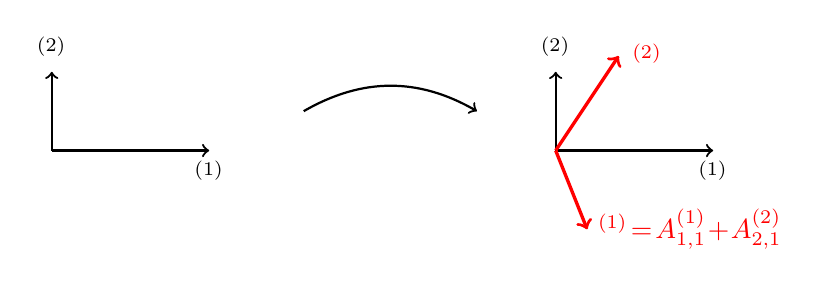
\begin{tikzpicture}[x=2cm]
			% LEFT: Standard basis vectors and unit square
			\begin{scope}
				\draw[->, thick] (0,0) -- (1,0) node[below] {$\vu^{(1)}$};
				\draw[->, thick] (0,0) -- (0,1) node[above] {$\vu^{(2)}$};
				%\draw[fill=gray!15] (0,0) -- (1,0) -- (1,1) -- (0,1) -- cycle;
				%\node at (0.5,0.5) {\small unit square};
				%\node at (0.5,-0.6) {standard basis};
			\end{scope}
			% RIGHT: Transformed basis vectors and parallelogram
			\begin{scope}[shift={(3.2,0)}]
				\draw[->, thick] (0,0) -- (1,0) node[below] {$\vv^{(1)}$};
				\draw[->, thick] (0,0) -- (0,1) node[above] {$\vv^{(2)}$};
				\coordinate (A) at (0.2,-1.0);
				\coordinate (B) at (0.4,1.2);
				\draw[->, very thick, red] (0,0) -- (A) node[below,right] {$\mA \vu^{(1)}\!=\!A_{1,1}\vv^{(1)}\!+\!A_{2,1}\vv^{(2)}$};
				\draw[->, very thick, red] (0,0) -- (B) node[right,xshift=1pt] {$\mA \vu^{(2)}$};
				%	\node[blue] at (0.25,1.25) {};
				%	\node at (0.8,-0.6) {transformed basis};
			\end{scope}
			% Arrow between plots
			\draw[->, thick] (1.6,0.5) to[bend left] node[midway, above] {$\mA$} (2.7,0.5);
			%	\draw[->, thick] (1.3,0.5) -- (2.4,0.5) node[midway, above] {$\mA$};
		\end{tikzpicture}
		\end{center}
		{\selectlanguage{greek}
		\caption{\foreignlanguage{greek}{Ένας πίνακας $\mA$ ορίζει μία} \selectlanguage{english}{\gls{linearmap}} \foreignlanguage{greek}{μεταξύ 
		δύο} \glsentryuserv{vectorspace}. \label{fig_matrix_dict}} }
		\end{figure}
		\foreignlanguage{greek}{Βλέπε επίσης:} \gls{modelparam}, \gls{linreg}, \gls{linearmap}, \gls{vectorspace}, \gls{dataset}, 
		\gls{datapoint}, \gls{feature}, \gls{label}, \gls{linmodel}. },
	first={\foreignlanguage{greek}{πίνακας}},
	text={\foreignlanguage{greek}{πίνακας}},
	type=math,
	user1={\foreignlanguage{greek}{πίνακας}}, %nominative
	user2={\foreignlanguage{greek}{πίνακα}}, %genitive
	user3={\foreignlanguage{greek}{πίνακα}}, %accusative
	user4={\foreignlanguage{greek}{πίνακες}}, %nominativepl
	user5={\foreignlanguage{greek}{πινάκων}}, %genitivepl
	user6={\foreignlanguage{greek}{πίνακες}} %accusativepl
}

\newglossaryentry{LapMat}
{name={\foreignlanguage{greek}{πίνακας} Laplace},
	description={\foreignlanguage{greek}{Η δομή ενός}\index{\foreignlanguage{greek}{πίνακας} Laplace} \glsentryuserii{graph} $\graph$,  
		\foreignlanguage{greek}{με κόμβους $\nodeidx=1, \,\ldots, \,\nrnodes$, μπορεί να αναλυθεί χρησιμοποιώντας τις ιδιότητες ειδικών}   
		\glsentryuserv{matrix} \foreignlanguage{greek}{που σχετίζονται με τον $\graph$. Ένας τέτοιος} \glsentryuseri{matrix} 
		\foreignlanguage{greek}{είναι ο} \glsentryuseri{matrix} Laplace \glsentryuserii{graph} $\mL^{(\graph)} \in \mathbb{R}^{\nrnodes \times \nrnodes}$, 
		\foreignlanguage{greek}{ο οποίος ορίζεται για έναν μη κατευθυνόμενο και σταθμισμένο} \glsentryuseriii{graph} \cite{Luxburg2007}, \cite{Ng2001}. 
		\foreignlanguage{greek}{Από άποψη στοιχείων ορίζεται ως (βλέπε Σχ.} \ref{fig_lap_mtx_dict})
		\begin{equation}
			\nonumber
			\LapMatEntry{\graph}{\nodeidx}{\nodeidx'} \defeq \begin{cases} - \edgeweight_{\nodeidx,\nodeidx'}, & \mbox{ for } \nodeidx\neq \nodeidx', \edge{\nodeidx}{\nodeidx'}\!\in\!\edges; \\ 
			\sum\limits_{\nodeidx'' \neq \nodeidx} \edgeweight_{\nodeidx,\nodeidx''}, & \mbox{ for } \nodeidx = \nodeidx'; \\ 
							0, & \mbox{ else.} \end{cases}
	 	\end{equation}
  		\foreignlanguage{greek}{Εδώ, $\edgeweight_{\nodeidx,\nodeidx'}$ δηλώνει το} \glsentryuseriii{edgeweight} \foreignlanguage{greek}{μίας 
		ακμής} $\edge{\nodeidx}{\nodeidx'} \in \edges$. 
 	 	\begin{figure}[H]
  		\begin{center}
    		\begin{minipage}{0.45\textwidth}
		\begin{tikzpicture}
				%	 				% 		% Left part - Graph
	 	 		\begin{scope}[every node/.style={circle, draw, minimum size=1cm}]
	 				\node (1) at (0,0) {1};
	 				\node (2) [below left=of 1] {2};
	 				\node (3) [below right=of 1] {3};
	 				\draw (1) -- (2);
	 				\draw (1) -- (3);
	 			\end{scope}
				\node at (0,-3) {(a)};
	 	\end{tikzpicture}
	 	\end{minipage} 
	 	\hspace*{-15mm}
 		\begin{minipage}{0.45\textwidth}
		\centering
	 			\begin{equation} 
	 				 \LapMat{\graph} = \begin{pmatrix} 2 & -1& -1 \\ -1& 1 & 0 \\  -1 & 0 & 1 \end{pmatrix}  
	 				 \nonumber
	 			\end{equation} 
				\begin{minipage}{\textwidth}
				\vspace{3.5ex}
				\centering
				{\selectfont (b)}
				\end{minipage}
	 	\end{minipage}
		{\selectlanguage{greek}
	 	\caption{\label{fig_lap_mtx_dict} \selectlanguage{english}{(a)} \foreignlanguage{greek}{Κάποιος μη κατευθυνόμενος} \glsentryuseri{graph} $\graph$ 
		 	\foreignlanguage{greek}{με τρεις κόμβους $\nodeidx=1,2,3$.} \selectlanguage{english}{(b)} \foreignlanguage{greek}{Ο} \glsentryuseri{matrix} 
			\selectlanguage{english}{Laplace} $\LapMat{\graph}  \in \mathbb{R}^{3 \times 3}$ 
			\foreignlanguage{greek}{του} $\graph$.} }
	 	\end{center}
	 	\end{figure}
		\foreignlanguage{greek}{Βλέπε επίσης:} \gls{graph}, \gls{matrix}, \gls{edgeweight}.},
	first={\foreignlanguage{greek}{πίνακας} Laplace},
	text={\foreignlanguage{greek}{πίνακας} Laplace},
	type=math,
	user1={\foreignlanguage{greek}{πίνακας} Laplace}, %nominative
  	user2={\foreignlanguage{greek}{πίνακα} Laplace} %genitive  
}

\newglossaryentry{covmtx}
{name={\foreignlanguage{greek}{πίνακας συνδιακύμανσης}}, 
	description={\foreignlanguage{greek}{Ο}\index{\foreignlanguage{greek}{πίνακας συνδιακύμανσης}} 
		\glsentryuseri{matrix} \glsentryuserii{covariance} (covariance matrix) \foreignlanguage{greek}{μίας} 
		\glsentryuserii{rv} $\featurevec \in \mathbb{R}^{\featuredim}$ \foreignlanguage{greek}{ορίζεται ως η} 
		\glsentryuseri{expectation} \foreignlanguage{greek}{(αν υφίσταται}):
		$$\covmtx{\featurevec} \defeq \expect \bigg \{ \big( \featurevec - \expect \big\{ \featurevec \big\} \big)  
		\big(\featurevec - \expect \big\{ \featurevec \big\} \big)\,^{T} \bigg\}.$$
		\\
		\foreignlanguage{greek}{Βλέπε επίσης:} \gls{covariance}, \gls{matrix}, \gls{rv}, \gls{expectation}.},
	first={\foreignlanguage{greek}{πίνακας συνδιακύμανσης}},
	text={\foreignlanguage{greek}{πίνακας συνδιακύμανσης}},
	type=math,
	user1={\foreignlanguage{greek}{πίνακας συνδιακύμανσης}}, %nominative
  	user2={\foreignlanguage{greek}{πίνακα συνδιακύμανσης}}, %genitive
	user3={\foreignlanguage{greek}{πίνακα συνδιακύμανσης}} %accusative   
}

\newglossaryentry{samplecovmtx}
{name={\foreignlanguage{greek}{πίνακας συνδιακύμανσης δείγματος}}, 
	description={\foreignlanguage{greek}{Θεωρούμε ένα} \glsentryuseriii{dataset} \foreignlanguage{greek}{που αποτελείται από} 
		\glsentryuservi{datapoint} \foreignlanguage{greek}{που χαρακτηρίζονται από} \glsentryuservi{featurevec} 
		$\featurevec^{(1)}, \,\ldots, \,\featurevec^{(\samplesize)} \in \mathbb{R}^{\nrfeatures}$.	
		\foreignlanguage{greek}{Ο}\index{\foreignlanguage{greek}{πίνακας συνδιακύμανσης δείγματος}} \glsentryuseri{covmtx} 
		\glsentryuserii{sample} (sample covariance matrix) \foreignlanguage{greek}{του} $\dataset$ \foreignlanguage{greek}{ορίζεται ως ο} 
		\glsentryuseri{covmtx} \foreignlanguage{greek}{αναφορικά με την} \glsentryuseriii{empiricaldistribution} $\probdist^{(\dataset)}$ 
		\foreignlanguage{greek}{που επάγεται από το $\dataset$. Δίνεται ρητά από} 
		$$\samplecovmtxgeneric = \frac{1}{\samplesize} \sum_{\sampleidx=1}^{\samplesize} (\featurevec^{(\sampleidx)}\!-\!\widehat{\vm}) (\featurevec^{(\sampleidx)}\!-\!\widehat{\vm})\,^{T}.$$ 
		\foreignlanguage{greek}{Εδώ χρησιμοποιούμε τη} \glsentryuseriii{samplemean} $\samplemeanvecgeneric$. 
		\\
		\foreignlanguage{greek}{Βλέπε επίσης:} \gls{dataset}, \glspl{datapoint}, \gls{featurevec}, \gls{sample}, \gls{covmtx},
		\gls{empiricaldistribution}, \gls{samplemean}.},
	first={\foreignlanguage{greek}{πίνακας συνδιακύμανσης δείγματος}},
	text={\foreignlanguage{greek}{πίνακας συνδιακύμανσης δείγματος}},
	type=math,
	user1={\foreignlanguage{greek}{πίνακας συνδιακύμανσης δείγματος}}, %nominative
	user2={\foreignlanguage{greek}{πίνακα συνδιακύμανσης δείγματος}}, %genitive 
	user3={\foreignlanguage{greek}{πίνακα συνδιακύμανσης δείγματος}} %accusative 
}

\newglossaryentry{fullrank}
{name={\foreignlanguage{greek}{πλήρους τάξης}},
 	description={TBC.\index{full-rank} }, 
	text={\foreignlanguage{greek}{πλήρους τάξης}},
  	first={\foreignlanguage{greek}{πλήρους τάξης}},
	type=math,
	user1={\foreignlanguage{greek}{πλήρους τάξης}} %genitive
}

\newglossaryentry{mvndist}
{name={\foreignlanguage{greek}{πολυμεταβλητή κανονική κατανομή}}, 
	description={TBC.\index{multivariate normal distribution} }, 
	first={\foreignlanguage{greek}{πολυμεταβλητή κανονική κατανομή}},
	text={\foreignlanguage{greek}{πολυμεταβλητή κανονική κατανομή}},
	type=math,
	user1={\foreignlanguage{greek}{πολυμεταβλητή κανονική κατανομή}}, %nominative
	user2={\foreignlanguage{greek}{πολυμεταβλητής κανονικής κατανομής}}, %genitive 
	user3={\foreignlanguage{greek}{πολυμεταβλητή κανονική κατανομή}}, %accusative 
	user4={\foreignlanguage{greek}{πολυμεταβλητές κανονικές κατανομές}}, %nominativepl
	user5={\foreignlanguage{greek}{πολυμεταβλητών κανονικών κατανομών}}, %genitivepl 
	user6={\foreignlanguage{greek}{πολυμεταβλητές κανονικές κατανομές}} %accusativepl 
}

\newglossaryentry{projgd}
{name={\foreignlanguage{greek}{προβεβλημένη κάθοδος κλίσης}},
	description={\foreignlanguage{greek}{Θεωρούμε μία μέθοδο βασισμένη στην} \glsentryuseriii{erm} \foreignlanguage{greek}{που 
		χρησιμοποιεί ένα παραμετροποιημένο} \glsentryuseriii{model} \foreignlanguage{greek}{με} \glsentryuseriii{paramspace} 
		$\paramspace \subseteq \mathbb{R}^{\dimlocalmodel}$. \foreignlanguage{greek}{Ακόμα και αν η} \glsentryuseri{objfunc} 
		\glsentryuserii{erm} \foreignlanguage{greek}{εί\-ναι} \glsentryuseri{smooth}, \foreignlanguage{greek}{δεν μπορούμε να 
		χρησιμοποιήσουμε τη βασική} \glsentryuseriii{gd}, \foreignlanguage{greek}{καθώς δεν λαμβάνει υπόψη περιορισμούς 
		στη μεταβλητή βελτιστοποίησης (δηλαδή τις} \glsentryuserix{modelparam}). 
		\foreignlanguage{greek}{Η προβεβλημένη}\index{\foreignlanguage{greek}{προβεβλημένη κάθοδος κλίσης}} \glsentryuseri{gd} 
		(projected gradient descent - projected GD) \foreignlanguage{greek}{επεκτείνει τη βασική} \glsentryuseriii{gd} 
		\foreignlanguage{greek}{για να αντιμετωπίσει αυτό το ζήτημα. Μία μοναδική επανάληψη της προβεβλημένης} \glsentryuserii{gd} 
		\foreignlanguage{greek}{περιλαμβάνει πρώτα τη λήψη ενός} \glsentryuserii{gradstep} \foreignlanguage{greek}{και στη συνέχεια την 
		προβολή του αποτελέσματος πίσω στον} \glsentryuseriii{paramspace}. \foreignlanguage{greek}{Βλέπε Σχ. \ref{fig_projected_GD_dict} 
		για μία οπτική απεικόνιση.}
		\begin{figure}[H]
		\begin{center}
			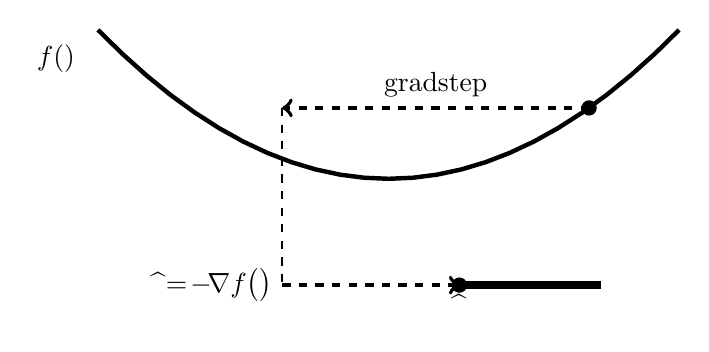
\begin{tikzpicture}[scale=0.9]
			\node [right] at (-5.1,1.7) {$f(\weights)$} ;
			\draw[ultra thick, domain=-4.1:4.1] plot (\x,  {(1/8)*\x*\x});
		%	\draw[dashed, thick, domain=1:3.6] plot (\x,  {\x - 1}) node[right] {$ f\big(\weights^{(\itercntr)}\big)\!+\!\big(\weights\!-\!\weights^{(\itercntr)}\big)^{T} \nabla f\big(\weights^{(\itercntr)}\big)$};
			\draw [fill] (2.83,1) circle [radius=0.1] node[right] {$\weights$};
			\draw[line width =0.5mm,dashed,->] (2.83,1) -- node[midway,above] {\glsentryuseri{gradstep}} (-1.5,1);
			\draw[line width =0.2mm,dashed] (-1.5,1) --(-1.5,-1.5)  node [below, left]{$\widehat{\weights}=\weights\!-\!\lrate \nabla f\big(\weights\big)$} ;
			\draw[line width =0.5mm,dashed,->] (-1.5,-1.5)  -- node[midway,above] {} (1,-1.5) ; 
			\draw [fill] (1,-1.5) circle [radius=0.1] node[below] {$\projection{\paramspace}{\widehat{\weights}}$};
			\draw[line width=1mm] (1,-1.5) -- (3,-1.5) node[midway, above] {$\paramspace$};
			\end{tikzpicture}
		\vspace*{-5mm}
		\end{center}
		{\selectlanguage{greek}
		\caption{\foreignlanguage{greek}{Η προβεβλημένη} \glsentryuseri{gd} \foreignlanguage{greek}{επαυξάνει ένα βασικό} 
			\glsentryuseriii{gradstep} \foreignlanguage{greek}{με μία} \glsentryuseriii{projection} \foreignlanguage{greek}{πίσω στο σύνολο 
			περιορισμών} $\paramspace$.}
		\label{fig_projected_GD_dict} }
		\end{figure}
		\foreignlanguage{greek}{Βλέπε επίσης:} \gls{erm}, \gls{model}, \gls{paramspace}, \gls{objfunc}, \gls{smooth}, \gls{gd}, \gls{modelparam}, 
		\gls{gradstep}, \gls{projection}.},
	first={\foreignlanguage{greek}{προβεβλημένη κάθοδος κλίσης}},
	text={\foreignlanguage{greek}{προβεβλημένη κάθοδος κλίσης}},
	type=math,
	user1={\foreignlanguage{greek}{προβεβλημένη κάθοδος κλίσης}}, %nominative
	user2={\foreignlanguage{greek}{προβεβλημένης καθόδου κλίσης}} %genitive 
}

\newglossaryentry{optproblem}
{name={\foreignlanguage{greek}{πρόβλημα βελτιστοποίησης}}, 
	description={\foreignlanguage{greek}{Ένα πρόβλημα βελτιστοποίησης}\index{\foreignlanguage{greek}{πρόβλημα βελτιστοποίησης}} 
		(optimization problem) \foreignlanguage{greek}{είναι μία μαθηματική δομή που αποτελείται από μία} \glsentryuseriii{objfunc} 
		$f: \mathcal{U} \rightarrow \mathcal{V}$ \foreignlanguage{greek}{ορισμένη πάνω σε μία μεταβλητή βελτιστοποίησης 
		$\weights \in \mathcal{U}$, μαζί με ένα εφικτό σύνολο $\mathcal{W} \subseteq \mathcal{U}$. Το 
		πεδίο τιμών $\mathcal{V}$ θεωρείται ότι είναι διατεταγμένο, που σημαίνει ότι για οποιαδήποτε δύο στοιχεία 
		$\mathbf{a}, \mathbf{b} \in \mathcal{V}$, μπορούμε να καθορίσουμε αν $\mathbf{a} < \mathbf{b}$, $\mathbf{a} = \mathbf{b}$, 
		ή $\mathbf{a} > \mathbf{b}$. Ο στόχος της βελτιστοποίησης είναι να βρούμε εκείνες τις τιμές $\weights \in \mathcal{W}$ 
		για τις οποίες η αντικειμενική $f(\weights)$ είναι ακρότατη—δηλαδή ελάχιστη ή μέγιστη} 
		\cite{BertsekasNonLinProgr}, \cite{BoydConvexBook}, \cite{nesterov04}.\\
		\foreignlanguage{greek}{Βλέπε επίσης:} \gls{objfunc}.},
	first={\foreignlanguage{greek}{πρόβλημα βελτιστοποίησης}},
	text={optimization problem},
	type=math,
	user1={\foreignlanguage{greek}{πρόβλημα βελτιστοποίησης}}, %nominative
  	user2={\foreignlanguage{greek}{προβλήματος βελτιστο\-ποί\-ησης}}, %genitive 
	user3={\foreignlanguage{greek}{πρόβλημα βελτιστοποίησης}} %accusative
}

\newglossaryentry{projection}
{name={\foreignlanguage{greek}{προβολή}}, 
       description={\foreignlanguage{greek}{Θεωρούμε ένα υποσύνολο}\index{\foreignlanguage{greek}{προβολή}} 
       		$\paramspace \subseteq \mathbb{R}^{\dimlocalmodel}$ \foreignlanguage{greek}{του $\dimlocalmodel$-διάστατου} 
		\glsentryuserii{euclidspace}. \foreignlanguage{greek}{Ορίζουμε την προβολή $\projection{\paramspace}{\weights}$ 
		ενός} \glsentryuserii{vector} $\weights \in \mathbb{R}^{\dimlocalmodel}$ \foreignlanguage{greek}{στο $\paramspace$ ως}
		\begin{equation} 
   	    		\nonumber
			\label{equ_def_proj_generic_dict}
  	     		\projection{\paramspace}{\weights} = \argmin_{\weights' \in \paramspace} \normgeneric{\weights - \weights'}{2}. 
         	\end{equation}
		 \foreignlanguage{greek}{Με άλλα λόγια, η $\projection{\paramspace}{\weights}$ είναι το} \glsentryuseri{vector} 
		 \foreignlanguage{greek}{στο $\paramspace$ που είναι πιο κοντά στο $\weights$. Η προβολή είναι καλά ορισμένη μόνο 
		 για υποσύνολα $\paramspace$ για τα οποία υφίσταται το παραπάνω} \glsentryuseri{minimum} \cite{BoydConvexBook}.\\
		 \foreignlanguage{greek}{Βλέπε επίσης:} \gls{euclidspace}, \gls{vector}, \gls{minimum}.},
	first={\foreignlanguage{greek}{προβολή}},
	text={\foreignlanguage{greek}{προβολή}},
	type=math,
	user1={\foreignlanguage{greek}{προβολή}}, %nominative
	user2={\foreignlanguage{greek}{προβολής}}, %genitive 
	user3={\foreignlanguage{greek}{προβολή}} %accusative 
}

\newglossaryentry{preimage}
{name={\foreignlanguage{greek}{προεικόνα}}, 
	description={\foreignlanguage{greek}{Θεωρούμε μία} \glsentryuseriii{function}\index{preimage} $f\colon \mathcal{U} \rightarrow \mathcal{V}$ 
		\foreignlanguage{greek}{μεταξύ δύο συνόλων. Η προεικόνα $f^{-1}(\mathcal{B})$ ενός υποσυνόλου $\mathcal{B} \subseteq \mathcal{V}$ 
		είναι το σύνολο όλων των εισόδων $u \in \mathcal{U}$ που αντιστοιχούνται στο $\mathcal{B}$ από την $f$, δηλαδή}
		\[
		f^{-1}(\mathcal{B}) \defeq \{ u \in \mathcal{U} \mid f(u) \in \mathcal{B} \}.
		\]
		\foreignlanguage{greek}{Η προεικόνα είναι καλά ορισμένη ακόμα και αν η} \glsentryuseri{function} $f$ \foreignlanguage{greek}{είναι 
		μη αντιστρέψιμη} \cite{RudinBookPrinciplesMatheAnalysis}. \\
		\foreignlanguage{greek}{Βλέπε επίσης:} \gls{function}. },
	first={\foreignlanguage{greek}{προεικόνα}},
	text={\foreignlanguage{greek}{προεικόνα}},
	type=math,
	user1={\foreignlanguage{greek}{προεικόνα}} %nominative
}

\newglossaryentry{conditionalexpect}
{name={\foreignlanguage{greek}{προσδοκία υπό συνθήκη}}, 
	description={TBC.\index{conditional expectation} }, 
 	first={\foreignlanguage{greek}{προσδοκία υπό συνθήκη}},  
 	text={\foreignlanguage{greek}{προσδοκία υπό συνθήκη}},
	type=math,
	user1={\foreignlanguage{greek}{προσδοκία υπό συνθήκη}}, %nominative
  	user2={\foreignlanguage{greek}{προσδοκίας υπό συνθήκη}}, %genitive 
	user3={\foreignlanguage{greek}{προσδοκία υπό συνθήκη}}, %accusative
	user4={\foreignlanguage{greek}{προσδοκίες υπό συνθήκη}}, %nominativepl
  	user5={\foreignlanguage{greek}{προσδοκιών υπό συνθήκη}}, %genitivepl 
	user6={\foreignlanguage{greek}{προσδοκίες υπό συνθήκη}} %accusativepl
}%υπό όρους

\newglossaryentry{proximable}
{name={\foreignlanguage{greek}{προσεγγίσιμος}},
	description={\foreignlanguage{greek}{Μία}\index{\foreignlanguage{greek}{προσεγγίσιμος}} 
		\glsentryuseriii{convex} \glsentryuseri{function} \foreignlanguage{greek}{για την οποία ο} \glsentryuseri{proxop} 
		\foreignlanguage{greek}{μπορεί να υπολογιστεί αποτελεσματικά αναφέρεται μερικές φορές ως 
		προσεγγίσιμη ή απλή} \cite{Condat2013}.\\
		\foreignlanguage{greek}{Βλέπε επίσης:} \gls{convex}, \gls{function}, \gls{proxop}.},
	first={\foreignlanguage{greek}{προσεγγίσιμος}},
	text={\foreignlanguage{greek}{προσεγγίσιμος}},
	type=math,
	user1={\foreignlanguage{greek}{προσεγγίσιμος}}, %nominative
	user2={\foreignlanguage{greek}{προσεγγίσιμου}} %genitive 
}

\newglossaryentry{sigmaalgebra}
{name={\foreignlanguage{greek}{$\sigma$-άλγεβρα}},
	description={TBC.\index{$\sigma$-algebra} },
	first={\foreignlanguage{greek}{$\sigma$-άλγεβρα}},
	text={\foreignlanguage{greek}{$\sigma$-άλγεβρα}},
	type=math,
	user1={\foreignlanguage{greek}{$\sigma$-άλγεβρα}}, %nominative
  	user2={\foreignlanguage{greek}{$\sigma$-άλγεβρας}}, %genitive 
	user3={\foreignlanguage{greek}{$\sigma$-άλγεβρα}} %accusative
}

\newglossaryentry{fixedpoint}
{name={\foreignlanguage{greek}{σταθερό σημείο}},
	description={TBC.\index{fixed point} },
	first={\foreignlanguage{greek}{σταθερό σημείο}},
	text={\foreignlanguage{greek}{σταθερό σημείο}},
	type=math,
	user1={\foreignlanguage{greek}{σταθερό σημείο}}, %nominative
  	user2={\foreignlanguage{greek}{σταθερού σημείου}}, %genitive 
	user3={\foreignlanguage{greek}{σταθερό σημείο}} %accusative
}

\newglossaryentry{stochastic}
{name={\foreignlanguage{greek}{στοχαστική}},
	description={\foreignlanguage{greek}{Αναφερόμαστε σε μία μέθοδο ως στοχαστιή}\index{stochastic} 
		\foreignlanguage{greek}{αν περιλαμβάνει μία τυχαία συνιστώσα ή διέπεται από πιθανοτικούς 
		νόμους. Οι μέθοδοι} \glsentryuserii{ml} \foreignlanguage{greek}{χρησιμοποιούν τυχαιότητα για να 
		μειώσουν την υπολογιστική πολυπλοκότητα (π.χ. βλέπε} \glsentryuseri{stochGD}) 
		\foreignlanguage{greek}{ή για να αποτυπώσουν την} \glsentryuseriii{uncertainty} 
		\foreignlanguage{greek}{σε} \glsentryuservi{probmodel}. \\
		\foreignlanguage{greek}{Βλέπε επίσης:} \gls{ml}, \gls{stochGD}, \gls{uncertainty}, \gls{probmodel}.},
	first={\foreignlanguage{greek}{στοχαστική}},
	text={\foreignlanguage{greek}{στοχαστική}}, 
	type=math,
	user1={\foreignlanguage{greek}{στοχαστική}}, %nominative
	user2={\foreignlanguage{greek}{στοχαστικής}}, %genitive
	user3={\foreignlanguage{greek}{στοχαστική}}, %accusative
	user4={\foreignlanguage{greek}{στοχαστικός}}, %nominativemasc
	user5={\foreignlanguage{greek}{στοχαστικού}}, %genitivemasc
	user6={\foreignlanguage{greek}{στοχαστικό}}, %accusativemasc
	user7={\foreignlanguage{greek}{στοχαστικές}}, %nominativeoraccusativeplfem
	user8={\foreignlanguage{greek}{στοχαστικών}} %genitiveplfemormasc
}

\newglossaryentry{stochproc}
{name={\foreignlanguage{greek}{στοχαστική διαδικασία}},
	description={\foreignlanguage{greek}{Μία} \glsentryuseri{stochastic}\index{\foreignlanguage{greek}{στοχαστική διαδικασία}} 
		\foreignlanguage{greek}{διαδικασία είναι μία συλλογή} \glsentryuserv{rv} \foreignlanguage{greek}{που ορίζονται πάνω 
		σε έναν κοινό} \glsentryuseriii{probspace} \foreignlanguage{greek}{και που έχουν δείκτες από κάποιο σύνολο}
		$\mathcal{I}$ \cite{Brockwell91}, \cite{GrayProbBook}, \cite{papoulis}. \foreignlanguage{greek}{Το σύνολο δεικτών 
		$\mathcal{I}$ συνήθως αναπαριστά χρόνο και χώρο, επιτρέποντάς μας να αναπαραστήσουμε τυχαία φαινόμενα που 
		εξελίσσονται στον χρόνο ή σε χωρικές διαστάσεις—για παράδειγμα, θόρυβο αισθητήρα ή οικονομικές χρονοσειρές}.
		\foreignlanguage{greek}{Οι} \glsentryuservii{stochastic} \foreignlanguage{greek}{διαδικασίες δεν περιορίζονται σε 
		χρονικά ή χωρικά περιβάλλοντα. Για παράδειγμα, τυχαίοι} \glsentryuseriv{graph} \foreignlanguage{greek}{όπως ο} 
		\gls{ergraph} \foreignlanguage{greek}{ή το} \glsentryuseri{sbm} \foreignlanguage{greek}{μπορούν επίσης να θεωρηθούν} 
		\glsentryuservii{stochastic} \foreignlanguage{greek}{διαδικασίες. Εδώ, το σύνολο δεικτών $\mathcal{I}$ αποτελείται 
		από ζεύγη κόμβων που ευρετηριάζουν} \glsentryuservi{rv} \foreignlanguage{greek}{των οποίων οι τιμές κωδικοποιούν 
		την παρουσία ή το βάρος μίας ακμής μεταξύ δύο κόμβων. Επιπλέον, οι} \glsentryuservii{stochastic} 
		\foreignlanguage{greek}{διαδικασίες προκύπτουν φυσικά στην ανάλυση} \glsentryuserv{stochalgorithm}, 
		\foreignlanguage{greek}{όπως της} \glsentryuserii{stochGD}, \foreignlanguage{greek}{οι οποίοι κατασκευάζουν μία 
		ακολουθία} \glsentryuserv{rv}. \\
		\foreignlanguage{greek}{Βλέπε επίσης:} \gls{stochastic}, \gls{rv}, \gls{probspace}, \gls{graph}, \gls{ergraph}, \gls{sbm},
		\gls{stochalgorithm}, \gls{stochGD}, \gls{uncertainty}, \gls{probmodel}.},
	first={\foreignlanguage{greek}{στοχαστική διαδικασία}},
	text={\foreignlanguage{greek}{στοχαστική διαδικασία}},
	type=math,
	user1={\foreignlanguage{greek}{στοχαστική διαδικασία}}, %nominative
  	user2={\foreignlanguage{greek}{στοχαστικής διαδικασίας}}, %genitive
	user3={\foreignlanguage{greek}{στοχαστική διαδικασία}} %accusative
}

\newglossaryentry{convergence}
{name={\foreignlanguage{greek}{σύγκλιση}},
	description={\foreignlanguage{greek}{Θεωρούμε μία}\index{\foreignlanguage{greek}{σύγκλιση}}
		\glsentryuseriii{sequence} $\big( a_{\sampleidx} \big)_{\sampleidx \in \mathbb{N}}$ 
		\foreignlanguage{greek}{με αριθμητικές τιμές $a_{\sampleidx} \in \mathbb{R}$. Λέμε ότι αυτή η} 
		\glsentryuseri{sequence} \foreignlanguage{greek}{συγκλίνει σε μία τιμή
       	 	$a^\star$ αν οι τιμές $a_{\sampleidx}$ γίνονται αυθαίρετα κοντινές στην 
		$a^\star$ για επαρκώς μεγάλους δείκτες $\sampleidx$. 
        		Από μαθηματική άποψη, η} \glsentryuseri{sequence} \foreignlanguage{greek}{συγκλίνει στην
		$a^\star$ αν} 
		\cite{RudinBook}, \cite{RudinBookPrinciplesMatheAnalysis}
        		\[
           	\forall \epsilon > 0, \; \exists N \in \mathbb{N} : \sampleidx > N \Rightarrow |a_{\sampleidx} - a^\star| < \epsilon.
        		\]
		\foreignlanguage{greek}{Δηλώνουμε τη σύγκλιση} (convergence) \foreignlanguage{greek}{μίας} 
		\glsentryuserii{sequence} \foreignlanguage{greek}{στην $a^\star$ με}
		\[
			\lim_{\sampleidx \to \infty} a_{\sampleidx} = a^\star.
		\]
		\begin{figure}[H] 
			\centering
			\begin{tikzpicture}[x=1.2cm, y=2cm, >=stealth]
			% Axes
			\draw[->] (0.5,0) -- (6.5,0) node[right] {$\sampleidx$};
			\draw[->] (0.5,0) -- (0.5,1.6) node[above] {$a_\sampleidx$};
			% Epsilon neighbourhood (ε = 0.1)
  			\def\eps{0.3}
  			\fill[gray!30, opacity=0.4] (0, {1-\eps}) rectangle (6.3, {1+\eps});
  			\draw[dotted] (0,{1+\eps}) -- (6.3,{1+\eps}) node[right] {$1+\varepsilon$};
  			\draw[dotted] (0,{1-\eps}) -- (6.3,{1-\eps}) node[right] {$1-\varepsilon$};
			% Limit line at 1
			\draw[dashed] (0,1) -- (6.3,1) node[right] {$\lim_{\sampleidx \to \infty} a_\sampleidx = 1$};
			% Sequence points (e.g. a_t = 1 - 0.6^t)
			\foreach \t in {1,...,6} {
				\pgfmathsetmacro{\at}{1 - 0.6^(\t)}
				\fill (\t,\at) circle (2pt);
			}
			% Tick marks at t = 1, 2, 3
 		     	\foreach \t in {1,2,3} {
    		    	\draw (\t,0.02) -- (\t,-0.02) node[below] {$\t$};
  		    	}
			% Indicate N (first index within ε-band)
  			\def\N{3}
  			\draw[densely dashed, thick, red] (\N,0) -- (\N,1.7);
  			\node[above] at (\N,1.7) {$N$};
			\end{tikzpicture}
		{\selectlanguage{greek}
		\caption{\foreignlanguage{greek}{Μία} \glsentryuseri{sequence} \foreignlanguage{greek}{πραγματικής 
			τιμής $\big( a_{\sampleidx} \big)_{\sampleidx \in \mathbb{N}}$ 
			που συγκλίνει στο όριο} $a^\star = 1$.\label{fig:convergence_dict}} }
		\end{figure} 
		\foreignlanguage{greek}{Η έννοια της σύγκλισης μίας} \glsentryuserii{sequence} 
		\foreignlanguage{greek}{πραγματικής τιμής (όπου $\mathcal{A}=\mathbb{R}$) επεκτείνεται φυσικά σε μία} 
		\glsentryuseriii{sequence} \foreignlanguage{greek}{σε έναν αυθαίρετο}
		\glsentryuseriii{metricspace} $\mathcal{A}$. \foreignlanguage{greek}{Πράγματι, χρειάζεται απλώς να 
		αντικαταστήσουμε την απόλυτη διαφορά $|a_{\sampleidx} - a^\star|$ με τη}
		\glsentryuseriii{metric} $\metric{a_{\sampleidx}}{a^\star}$. 
		\foreignlanguage{greek}{Σημείωση ότι μία} \glsentryuseri{sequence} \foreignlanguage{greek}{μπορεί να 
		συγκλίνει μόνο αν είναι μία} \glsentryuseri{cauchysequence} \cite{RudinBookPrinciplesMatheAnalysis}. 
		\foreignlanguage{greek}{Ωστόσο, δε συγκλίνει κάθε} \glsentryuseri{cauchysequence}, 
		\foreignlanguage{greek}{εκτός αν ο υποκείμενος} \glsentryuseri{metricspace} \foreignlanguage{greek}{είναι πλήρης}. 
		\\
		\foreignlanguage{greek}{Βλέπε επίσης:} \gls{sequence}, \gls{metricspace}, \gls{metric}, \gls{cauchysequence}. },
	first={\foreignlanguage{greek}{σύγκλιση}},
	text={\foreignlanguage{greek}{σύγκλιση}},
	type=math, 
	user1={\foreignlanguage{greek}{σύγκλιση}}, %nominative
	user2={\foreignlanguage{greek}{σύγκλισης}}, %genitive 
	user3={\foreignlanguage{greek}{σύγκλιση}} %accusative
}

\newglossaryentry{symmetricmatrix}
{name={\foreignlanguage{greek}{συμμετρικός πίνακας}},
	description={TBC.\index{symmetric matrix} },
	first={\foreignlanguage{greek}{συμμετρικός πίνακας}},
	text={\foreignlanguage{greek}{συμμετρικός πίνακας}},
	type=math, 
	user1={\foreignlanguage{greek}{συμμετρικός πίνακας}}, %nominative
	user2={\foreignlanguage{greek}{συμμετρικού πίνακα}}, %genitive 
	user3={\foreignlanguage{greek}{συμμετρικό πίνακα}} %accusative
}

\newglossaryentry{function}
{name={\foreignlanguage{greek}{συνάρτηση}},
	description={\foreignlanguage{greek}{Μία συνάρτηση} (function)\index{\foreignlanguage{greek}{συνάρτηση}} 
		\foreignlanguage{greek}{μεταξύ δύο συνόλων $\mathcal{U}$ και $\mathcal{V}$ αποδίδει σε κάθε στοιχείο  
		$u \in \mathcal{U}$ ακριβώς ένα στοιχείο} $f(u) \in \mathcal{V}$ \cite{RudinBookPrinciplesMatheAnalysis}. 
		\foreignlanguage{greek}{Το γράφουμε αυτό ως $$f: \mathcal{U} \rightarrow \mathcal{V}: u \mapsto f(u),$$ 
		όπου $\mathcal{U}$ είναι το} \glsentryuseri{domain} \foreignlanguage{greek}{και $\mathcal{V}$ το} 
		\glsentryuseri{co-domain} \foreignlanguage{greek}{της $f$. Για την ακρίβεια, η συνάρτηση $f$ ορίζει μία μοναδική} 
		\glsentryuseriii{output} $f(u) \in \mathcal{V}$ \foreignlanguage{greek}{για κάθε είσοδο $u \in \mathcal{U}$
		(βλέπε Σχ.} \ref{fig_function_dict}). 
		\begin{figure}[H]
			\centering
			\begin{tikzpicture}[>=stealth, node distance=1.2cm and 2.5cm]
				\tikzset{dot/.style={circle, fill=black, inner sep=1.2pt}}
				\node (A) [dot, label=left:$a$] {};
				\node (B) [dot, below=of A, label=left:$b$] {};
				\node (C) [dot, below=of B, label=left:$c$] {};
				\node (1) [dot, right=4cm of A, label=right:$\star$] {};
				\node (2) [dot, below=of 1, label=right:$\circ$] {};
				\node (3) [dot, below=of 2, label=right:$\otimes$] {};
				\node[draw=blue!70, thick, ellipse, inner sep=0.5cm, fit=(A)(B)(C), label=above:$\mathcal{U}$] {};
				\node[draw=green!70!black, thick, ellipse, inner sep=0.5cm, fit=(1)(2)(3), label=above:$\mathcal{V}$] {};
				\draw[->] (A) -- (2);
				\draw[->] (B) -- (1);
				\draw[->] (C) -- (2);
			\end{tikzpicture}			
		{\selectlanguage{greek}
		\caption{\foreignlanguage{greek}{Μία συνάρτηση \( f \colon \mathcal{U} \to \mathcal{V} \) που αντιστοιχίζει κάθε στοιχείο 
			του} \glsentryuserii{domain} $\mathcal{U} =  \{a,b,c\}$ \foreignlanguage{greek}{σε ακριβώς ένα στοιχείο του} 
			\glsentryuserii{co-domain} $\mathcal{V} = \{\star,\circ,\otimes\}$. 
			\label{fig_function_dict} } }
		\end{figure} 
		\foreignlanguage{greek}{Βλέπε επίσης:} \gls{domain}, \gls{co-domain}, \gls{output}. },
	first={\foreignlanguage{greek}{συνάρτηση}},
	text={\foreignlanguage{greek}{συνάρτηση}},
	type=math,
	user1={\foreignlanguage{greek}{συνάρτηση}}, %nominative
  	user2={\foreignlanguage{greek}{συνάρτησης}}, %genitive 
	user3={\foreignlanguage{greek}{συνάρτηση}}, %accusative
	user4={\foreignlanguage{greek}{συναρτήσεις}}, %nominativepl
  	user5={\foreignlanguage{greek}{συναρτήσεων}}, %genitivepl 
	user6={\foreignlanguage{greek}{συναρτήσεις}} %accusativepl
}

\newglossaryentry{pmf}
{name={\foreignlanguage{greek}{συνάρτηση μάζας πιθανότητας}}, 
	description={TBC.\index{probability mass function (pmf)} },
	first={\foreignlanguage{greek}{συνάρτηση μάζας πιθανότητας}},
	text={\foreignlanguage{greek}{συνάρτηση μάζας πιθανότητας}},
	type=math,
	user1={\foreignlanguage{greek}{συνάρτηση μάζας πιθανότητας}}, %nominative
  	user2={\foreignlanguage{greek}{συνάρτησης μάζας πιθανότητας}}, %genitive 
	user3={\foreignlanguage{greek}{συνάρτηση μάζας πιθανότητας}} %accusative
}

\newglossaryentry{pdf}
{name={\foreignlanguage{greek}{συνάρτηση πυκνότητας πιθανότητας}},
	description={\foreignlanguage{greek}{Η συνάρτηση πυκνότητας 
		πιθανότητας}\index{\foreignlanguage{greek}{συνάρτηση πυκνότητας πιθανότητας}} (probability density function - pdf) 
		$\pdf{\feature}{\cdot}$ \foreignlanguage{greek}{μίας} \glsentryuserii{continuous} \glsentryuserii{rv} 
		\foreignlanguage{greek}{πραγματικής τιμής $\feature \in \mathbb{R}$ μας επιτρέπει να υπολογίσουμε την} 
		\glsentryuseriii{probability} $\prob{\feature \in \mathcal{B}}$ (\foreignlanguage{greek}{του} \glsentryuserii{event} 
		$\mathcal{B} \subseteq \mathbb{R}$) \foreignlanguage{greek}{μέσω ενός} \glsentryuserii{LebesgueIntegral} \foreignlanguage{greek}{ως 
		εξής} \cite[\foreignlanguage{greek}{Κεφ.} 3]{BertsekasProb}:
		%is a particular representation of its \gls{probdist}. If the pdf exists, 
		%it can be used to compute the \gls{probability} that $\feature$ takes 
		%on a value from a \gls{measurable} set $\mathcal{B} \subseteq \mathbb{R}$ 
	 	$$\prob{\feature \in \mathcal{B}} = \int_{\mathcal{B}} \pdf{\feature}{\eta} d 
	 	\eta.$$  
		\foreignlanguage{greek}{Αυτός ο ορισμός επεκτείνεται φυσικά σε μία} (\glsentryuseriii{continuous}) \glsentryuseriii{rv} 
		\glsentryuserviii{vector} \foreignlanguage{greek}{τιμής $\featurevec \in \mathbb{R}^{\nrfeatures}$, καθώς το} 
		\glsentryuseri{LebesgueIntegral} \foreignlanguage{greek}{ορίζεται για τον $\mathbb{R}^{\nrfeatures}$ με οποιαδήποτε} 
		\glsentryuseriii{dimension} $\nrfeatures$. 
		%If the pdf of a \gls{vector}-valued \gls{rv} $\featurevec \in \mathbb{R}^{\featuredim}$ exists, 
		%it allows us to compute the \gls{probability} of $\featurevec$ belonging to a 
		%\gls{measurable} region $\mathcal{R}$ via 
    		%$\prob{\featurevec \in \mathcal{R}} = \int_{\mathcal{R}} p(\featurevec') d \feature_{1}' \,\ldots \,d \feature_{\featuredim}' $ \cite[Ch. 3]{BertsekasProb}.
		\\
        		\foreignlanguage{greek}{Βλέπε επίσης:} \gls{continuous}, \gls{rv}, \gls{probability}, \gls{event}, \gls{LebesgueIntegral}, \gls{vector}, 
		\gls{dimension}, \gls{probdist}, \gls{measurable}.},
	first={\foreignlanguage{greek}{συνάρτηση πυκνότητας πιθανότητας}},
	text={\foreignlanguage{greek}{συνάρτηση πυκνότητας πιθανότητας}},
	type=math,
	user1={\foreignlanguage{greek}{συνάρτηση πυκνότητας πιθανότητας}}, %nominative
	user2={\foreignlanguage{greek}{συνάρτησης πυκνότητας πιθανότητας}}, %genitive
	user3={\foreignlanguage{greek}{συνάρτηση πυκνότητας πιθανότητας}} %accusative    
}

\newglossaryentry{covariance}
{name={\foreignlanguage{greek}{συνδιακύμανση}}, 
	description={TBC.\index{covariance} },
	first={\foreignlanguage{greek}{συνδιακύμανση}},
	text={\foreignlanguage{greek}{συνδιακύμανση}},
	type=math,
	user1={\foreignlanguage{greek}{συνδιακύμανση}}, %nominative
  	user2={\foreignlanguage{greek}{συνδιακύμανσης}} %genitive
}

\newglossaryentry{connected}
{name={\foreignlanguage{greek}{συνεκτικός}}, 
description={\foreignlanguage{greek}{Ένας}\index{connected} 
		\glsentryuseri{undirectedgraph} $\graph=\pair{\nodes}{\edges}$ \foreignlanguage{greek}{είναι συνεκτικός 
		αν, για κάθε μη κενό υποσύνολο $\nodes' \subset \nodes$, μπορούμε να βρούμε τουλάχιστον 
		μία ακμή που συνδέει έναν κόμβο στο $\nodes'$ με κάποιον κόμβο στο $\nodes \setminus \nodes'$.
		Παρουσιάζουμε δύο παραδείγματα} \glsentryuserv{undirectedgraph} \foreignlanguage{greek}{στο Σχ.} 
		\ref{fig_connected_dict}.
		\begin{figure}[H]
			\centering
			\begin{tikzpicture}
			% Horizontal axis
			% Left graph (single edge)
			\node[circle, fill=black, inner sep=1.5pt, label=above:{1}] (A1) at (0, 1.5) {};
			\node[above=0.5cm of A1, align=center] {\foreignlanguage{greek}{μη συνεκτικός}};
			\node[circle, fill=black, inner sep=1.5pt, label=below right:{2}] (B1) [below right=0.8cm and 0.5cm of A1] {};
			\node[circle, fill=black, inner sep=1.5pt, label=below left:{3}] (C1) [below left=0.8cm and 0.5cm of A1] {};
			\draw [line width=1 pt]  (A1) -- (B1);
			\node at (0, -1) {(a)};
			% Middle graph (two edges, shifted right)
			\begin{scope}[xshift=3.5cm]
				\node[circle, fill=black, inner sep=1.5pt, label=above:{1}] (A2) at (0, 1.5) {};
				\node[above=0.5cm of A2, align=center] {\foreignlanguage{greek}{συνεκτικός}};
				\node[circle, fill=black, inner sep=1.5pt, label=below right:{2}] (B2) [below right=0.8cm and 0.5cm of A2] {};
				\node[circle, fill=black, inner sep=1.5pt, label=below left:{3}] (C2) [below left=0.8cm and 0.5cm of A2] {};
				\draw [line width=1 pt]  (A2) -- (B2);
				\draw [line width=1 pt]  (B2) -- (C2);
				\node at (0, -1) {(b)};
			\end{scope}
			\end{tikzpicture}
		{\selectlanguage{greek}
		\caption{\selectlanguage{english}{(a)} \foreignlanguage{greek}{Ένας} \glsentryuseri{graph} \foreignlanguage{greek}{που είναι 
			μη συνεκτικός.} \selectlanguage{english}{(b)} \foreignlanguage{greek}{Ένας} \glsentryuseri{graph} 
			\foreignlanguage{greek}{που είναι συνεκτικός}. \label{fig_connected_dict}} }
		\end{figure} 
		\foreignlanguage{greek}{Βλέπε επίσης:} \gls{undirectedgraph}, \gls{graph}, \gls{algconn}.}, 
	first={\foreignlanguage{greek}{συνεκτικός}},
	text={\foreignlanguage{greek}{συνεκτικός}},
	type=math,
	user1={\foreignlanguage{greek}{συνεκτικός}}, %nominative
	user2={\foreignlanguage{greek}{συνεκτικού}} %genitive  
}

\newglossaryentry{continuous}
{name={\foreignlanguage{greek}{συνεχής}}, 
	description={TBC.\index{continuous} },
	first={\foreignlanguage{greek}{συνεχής}},
	text={\foreignlanguage{greek}{συνεχής}},
	type=math,
	user1={\foreignlanguage{greek}{συνεχής}}, %nominativemascandfem
	user2={\foreignlanguage{greek}{συνεχούς}}, %genitivemascandfem
	user3={\foreignlanguage{greek}{συνεχή}}, %accusativemascandfem
	user4={\foreignlanguage{greek}{συνεχείς}}, %nominativeplmascandfem
	user5={\foreignlanguage{greek}{συνεχών}}, %genitiveplmascandfem
	user6={\foreignlanguage{greek}{συνεχείς}} %accusativeplmascandfem
}

\newglossaryentry{contractop}
{name={\foreignlanguage{greek}{συστολικός τελεστής}},
	description={\foreignlanguage{greek}{Ένας}\index{contractive operator} \glsentryuseri{operator} 
		$\fixedpointop: \mathcal{V} \rightarrow  \mathcal{V}$ \foreignlanguage{greek}{σε έναν} \glsentryuseriii{normedspace} 
		$(\mathcal{V}, \normgeneric{\,\cdot \,}{})$
		\foreignlanguage{greek}{λέγεται συστολή (ή συστολικός} (contractive operator)) \foreignlanguage{greek}{αν, 
		για κάποιον} $\contractfac \in [0,1)$, \cite{BausckeCombette}, \cite{ProximalMethods}
		\begin{equation} 
			\nonumber
			\normgeneric{ \fixedpointop \weights\!-\!\fixedpointop \weights'}{}  \leq 
			 \contractfac	\normgeneric{\weights\!-\!\weights'}{} \quad \mbox{\foreignlanguage{greek}{ισχύει για κάθε} } \weights,\weights' \in \mathcal{V}.
		\end{equation} 
		\foreignlanguage{greek}{Η έννοια του συστολικού} \glsentryuserii{operator} \foreignlanguage{greek}{γενικεύει φυσικά από} 
		\glsentryuservi{normedspace} \foreignlanguage{greek}{σε αυθαί\-ρετους} \glsentryuservi{metricspace} \cite{BausckeCombette}.
		\begin{figure}[H]
    			\centering
    			\begin{tikzpicture}[>=Latex, font=\small]
        			% Styles
        			\tikzset{
            		space/.style={draw, thick, circle, minimum size=4.0cm},
            		pt/.style={circle, inner sep=1.5pt, draw, fill=black},
            		maparrow/.style={->, very thick},
            		distline/.style={dashed, thick}
        			}
        			% Single space
        			\node[space,label=above:{$\featurespace$}] (X) at (0,0) {};
        			% Two points and their images under T inside the same space
        			\coordinate (x1)  at (-1.0,0.8);
        			\coordinate (x2)  at ( 1.0,0.8);
        			\coordinate (Tx1) at (-0.5,0.1);
        			\coordinate (Tx2) at ( 0.5,0.1);
        			% Points x, x'
        			\node[pt,label=above left:{$\featurevec$}] at (x1) {};
        			\node[pt,label=above right:{$\featurevec'$}] at (x2) {};
        			% Images T(x), T(x')
        			\node[pt] (TX1) at (Tx1) {};
        			\node[pt] (TX2) at (Tx2) {};
        			\node[anchor=east] at ($(TX1.west)+(-4pt,-2pt)$) {$\fixedpointop \featurevec$};
        			\node[anchor=west] at ($(TX2.east)+(4pt,-2pt)$) {$\fixedpointop \featurevec'$};
        			% Contraction effect: distances shrink
        			\draw[distline] (x1) -- (x2)
            		node[midway, above=4pt] {$\metric{\featurevec}{\featurevec'}$};
        			\draw[distline] (Tx1) -- (Tx2)
            		node[midway, below=4pt] {$\metric{\fixedpointop \featurevec}{\fixedpointop \featurevec'}$};
        			% Fixed point in the same space
        			\coordinate (xs) at (0,-0.9);
        			\node[pt,label=below:{$\featurevec^\star$}] (XS) at (xs) {};
        			% Small loop indicating T(x*) = x*
        			%\draw[maparrow,shorten >=2pt,shorten <=2pt]
            		%(XS) .. controls +(60:0.7) and +(120:0.7) .. (XS);
        			\node at (0,-1.6) {$\fixedpointop \featurevec^\star = \featurevec^\star$};
    			\end{tikzpicture}
    		{\selectlanguage{greek}
		\caption{\foreignlanguage{greek}{Ένας συστολικός} \glsentryuseri{operator} $\fixedpointop:\featurespace\to\featurespace$ 
      			\foreignlanguage{greek}{έχει ένα μοναδικό} \glsentryuseriii{fixedpoint} $\featurevec^\star$ 
			\foreignlanguage{greek}{με $\fixedpointop \featurevec^\star=\featurevec^\star$.
      			Για οποιαδήποτε δύο σημεία $\featurevec,\featurevec'$ στον ίδιο χώρο, η απόσταση μεταξύ των εικόνων τους 
      			$\fixedpointop\featurevec$ και $\fixedpointop\featurevec'$ είναι αυστηρά μικρότερη}.}
    			\label{fig:contract_dict} }
		\end{figure}
		\foreignlanguage{greek}{Ενστικτωδώς, ένας συστολικός} \glsentryuseri{operator} \foreignlanguage{greek}{φέρνει 
		οποιαδήποτε δύο σημεία από το} \glsentryuseriii{domain} \foreignlanguage{greek}{του πιο κοντά μεταξύ τους τουλάχιστον 
		κατά έναν παράγοντα} $\contractfac$.
		\\ 
		\foreignlanguage{greek}{Βλέπε επίσης:} \gls{operator}, \gls{metricspace}, \gls{fixedpoint}, \gls{domain}. },
	first={\foreignlanguage{greek}{συστολικός τελεστής}},
	text={\foreignlanguage{greek}{συστολικός τελεστής}}, 
	type=math,
	user1={\foreignlanguage{greek}{συστολικός τελεστής}}, %nominative
	user2={\foreignlanguage{greek}{συστολικού τελεστή}}, %genitive
	user3={\foreignlanguage{greek}{συστολικό τελεστή}} %accusative
}%συναίρεση

\newglossaryentry{rank}
{name={\foreignlanguage{greek}{τάξη}},
	description={TBC.\index{rank} }, 
	text={\foreignlanguage{greek}{τάξη}},
	first={\foreignlanguage{greek}{τάξη}},
	type=math,
	user1={\foreignlanguage{greek}{τάξη}}, %nominative
	user2={\foreignlanguage{greek}{τάξης}}, %genitive
	user3={\foreignlanguage{greek}{τάξη}} %accusative
}

\newglossaryentry{operator} 
{name={\foreignlanguage{greek}{τελεστής}}, 
	description={\foreignlanguage{greek}{Ένας τελεστής} (operator) \foreignlanguage{greek}{είναι 
		μία}\index{\foreignlanguage{greek}{τελεστής}} \glsentryuseri{function} \foreignlanguage{greek}{της οποίας το}
		\glsentryuseri{domain} \foreignlanguage{greek}{και το} \glsentryuseri{co-domain} 
		\foreignlanguage{greek}{διαθέτουν μία συγκεκριμένη μαθηματική δομή, όπως έναν}  
		\glsentryuseriii{vectorspace}, \foreignlanguage{greek}{έναν} \glsentryuseriii{hilbertspace},
		\foreignlanguage{greek}{ή έναν} \glsentryuseriii{metricspace} \cite{Bauschke:2017}, \cite{DunfordSchwartz1988}. 
		\foreignlanguage{greek}{Πολλές μέθοδοι} \glsentryuserii{ml} \foreignlanguage{greek}{περιλαμβάνουν 
		τελεστές των οποίων το} \glsentryuseri{domain} \foreignlanguage{greek}{και το} \glsentryuseri{co-domain} 
		\foreignlanguage{greek}{είναι} \glsentryuseriv{euclidspace}.  
		\\ 
		\foreignlanguage{greek}{Βλέπε επίσης:} \gls{function}, \gls{domain}, \gls{co-domain}, \gls{vectorspace}, 
		\gls{hilbertspace}, \gls{metricspace}, \gls{ml}, \gls{euclidspace}.},
	first={\foreignlanguage{greek}{τελεστής}},
	text={\foreignlanguage{greek}{τελεστής}},
	type=math,
	user1={\foreignlanguage{greek}{τελεστής}}, %nominative
	user2={\foreignlanguage{greek}{τελεστή}}, %genitive 
	user3={\foreignlanguage{greek}{τελεστή}}, %accusative 
	user4={\foreignlanguage{greek}{τελεστές}}, %nominative
	user5={\foreignlanguage{greek}{τελεστών}}, %genitive 
	user6={\foreignlanguage{greek}{τελεστές}} %accusative 
}

\newglossaryentry{proxop}
{name={\foreignlanguage{greek}{τελεστής εγγύτητας}},
	description={\foreignlanguage{greek}{Δεδομένης μίας}\index{\foreignlanguage{greek}{εγγύς τελεστής}} 
		\glsentryuseriv{convex} \glsentryuserii{function} $f(\weights')$, \foreignlanguage{greek}{ορίζουμε τον τελεστή εγγύτητάς της ως} \cite{ProximalMethods}, \cite{Bauschke:2017} 
		$$\proximityop{f(\cdot)}{\weights}{\rho}\defeq \argmin_{\weights' \in \mathbb{R}^{\dimlocalmodel}} \bigg[ f(\weights')\!+\!\frac{\rho}{2} \normgeneric{\weights- \weights'}{2}^{2}\bigg] \mbox{ \foreignlanguage{greek}{με} } \rho > 0. $$ 
		\foreignlanguage{greek}{Όπως απεικονίζεται στο Σχ.} \ref{fig_proxoperator_opt_dict}, \foreignlanguage{greek}{η αξιολόγηση του τελεστή εγγύτητας 
		ισοδυναμεί με την ελαχιστοποίηση μίας παραλλαγής της $f(\weights')$ που έχει επιβληθεί ως ποινή. Ο όρος ποινής είναι η ανηγμένη 
		τετραγωνική Ευκλεί\-δεια απόσταση σε ένα δεδομένο} \glsentryuseriii{vector} $\weights$ (\foreignlanguage{greek}{το οποίο είναι η είσοδος στον 
		τελεστή εγγύτητας). 
		Ο τελεστής εγγύτητας μπορεί να ερμηνευτεί ως μία} \glsentryuseri{generalization} \foreignlanguage{greek}{του} \glsentryuserii{gradstep}, 
		\foreignlanguage{greek}{το οποίο ορίζεται ως μία} \glsentryuseri{smooth} \glsentryuseriii{convex} \glsentryuseri{function} $f(\weights')$. 
		\foreignlanguage{greek}{Πράγματι, η εκτέλεση ενός} \glsentryuserii{gradstep} \foreignlanguage{greek}{με} \glsentryuseriii{stepsize} $\lrate$ 
		\foreignlanguage{greek}{στο τρέχον} \glsentryuseriii{vector} $\weights$ \foreignlanguage{greek}{είναι το ίδιο με την εφαρμογή 
		του τελεστή εγγύτητας της } \glsentryuserii{function} $\tilde{f}(\weights')= \big( \nabla f(\weights)\big)\,^{T} (\weights'-\weights)$ 
		\foreignlanguage{greek}{και τη χρήση} $\rho=1/\lrate$.
			\begin{figure}[H]
			\begin{center}
				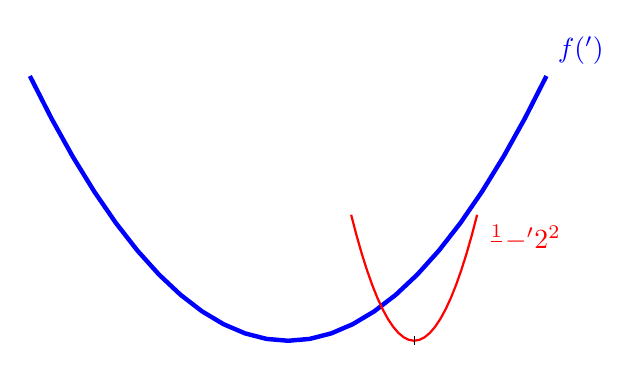
\begin{tikzpicture}[scale=0.8]
					% Original quadratic function
					\draw[blue, ultra thick, domain=-4.1:4.1] plot (\x, {(1/4)*\x*\x}) node[above right] {$f(\weights')$};		
					% Quadratic function with larger curvature, centered at w = 2
					\draw[red, thick, domain=1:3] plot (\x, {2*(\x - 2)*(\x - 2)}) node[below right] {$\frac{1}{\lrate}\normgeneric{\weights-\weights'}{2}^{2}$};
					% Axes
					% Minimum point of second curve
					\draw[shift={(2,0)}] (0pt,2pt) -- (0pt,-2pt) node[below] {$\weights$};
					%\node at (2,0.5) [anchor=north] {$\weights$};
				\end{tikzpicture}
			\end{center}
			{\selectlanguage{greek}
			\caption{\foreignlanguage{greek}{Ο τελεστής εγγύτητας ενημερώνει ένα} \glsentryuseriii{vector} $\weights$ 
				\foreignlanguage{greek}{ελαχιστοποιώντας μία εκδοχή της} \glsentryuserii{function} $f(\cdot)$ \foreignlanguage{greek}{που έχει 
				επιβληθεί ως ποινή. Ο όρος ποινής είναι η ανηγμένη τετραγωνική Ευκλείδεια απόσταση μεταξύ της μεταβλητής 
				βελτιστοποίησης $\weights'$ και του δεδομένου} \glsentryuserii{vector} $\weights$.	\label{fig_proxoperator_opt_dict}} }
		\end{figure}
		\foreignlanguage{greek}{Βλέπε επίσης:} \gls{convex}, \gls{function}, \gls{vector}, \gls{generalization}, \gls{gradstep}, \gls{smooth}, \gls{stepsize}.},
	first={\foreignlanguage{greek}{τελεστής εγγύτητας}},
	text={\foreignlanguage{greek}{τελεστής εγγύτητας}},
	type=math,
	user1={\foreignlanguage{greek}{τελεστής εγγύτητας}} %nominative
}

\newglossaryentry{rv}
{name={\foreignlanguage{greek}{τυχαία μεταβλητή}},
	description={\foreignlanguage{greek}{Μία τυχαία μεταβλητή}\index{\foreignlanguage{greek}{τυχαία μεταβλητή}} (random variable - RV) 
		\foreignlanguage{greek}{είναι μία} \glsentryuseri{function} \foreignlanguage{greek}{που αντιστοιχίζει τα} \glsentryuservi{outcome} 
		\foreignlanguage{greek}{ενός} \glsentryuserii{randomexperiment} \foreignlanguage{greek}{σε στοιχεία ενός} \glsentryuserii{measurable} 
		\foreignlanguage{greek}{χώρου} \cite{BillingsleyProbMeasure}, \cite{GrayProbBook}. 
 		\foreignlanguage{greek}{Από μαθηματική άποψη, μία τυχαία μεταβλητή είναι μία} \glsentryuseri{function} 
		$x: \samplespace \rightarrow \featurespace$ \foreignlanguage{greek}{της οποίας το} \glsentryuseri{domain} \foreignlanguage{greek}{είναι
		ο} \glsentryuseri{samplespace} $\samplespace$ \foreignlanguage{greek}{ενός} \glsentryuserii{probspace} \foreignlanguage{greek}{και 
		της οποίας το} \glsentryuseri{co-domain} \foreignlanguage{greek}{είναι ένας} \glsentryuseri{measurable} \foreignlanguage{greek}{χώρος
		$\featurespace$. Διαφορετικοί τύποι τυχαίων μεταβλητών περιλαμβάνουν}   
 		\begin{itemize} 
			\item {\foreignlanguage{greek}{δυαδικές τυχαίες μεταβλητές}}, \foreignlanguage{greek}{οι οποίες αντιστοιχίζουν κάθε} 
				\glsentryuseriii{outcome} \foreignlanguage{greek}{σε ένα στοιχείο ενός δυαδικού συνόλου (π.χ. $\{-1,1\}$ ή}\linebreak 
				$\{\text{\foreignlanguage{greek}{γάτα}}, \text{\foreignlanguage{greek}{όχι γάτα}}\}$)·
			\item {\glsentryuseriv{discreteRV}}, \foreignlanguage{greek}{οι οποίες παίρνουν τιμές σε ένα} \glsentryuseriii{countable} 
				\foreignlanguage{greek}{σύνολο (το οποίο μπορεί να είναι πεπερασμένο ή αριθμήσιμα άπειρο})·
 			\item {\foreignlanguage{greek}{τυχαίες μεταβλητές πραγματικής τιμής}}, \foreignlanguage{greek}{οι οποίες παίρνουν τιμές 
				στους πραγματικούς αριθμούς} $\mathbb{R}$·  
 			\item {\foreignlanguage{greek}{τυχαίες μεταβλητές} \glsentryuserviii{vector} \foreignlanguage{greek}{τιμής}}, 
				\foreignlanguage{greek}{οι οποίες αντιστοιχίζουν} \glsentryuservi{outcome} \foreignlanguage{greek}{στον} 
				\glsentryuseriii{euclidspace} $\mathbb{R}^{\featuredim}$.  
 		\end{itemize} 
 		\foreignlanguage{greek}{Η θεωρία} \glsentryuserv{probability} \foreignlanguage{greek}{χρησιμοποιεί την έννοια των} 
		\glsentryuserv{measurable} \foreignlanguage{greek}{χώρων για να ορίσει ενδελεχώς και να μελετήσει τις ιδιότητες συλλογών 
		τυχαίων μεταβλητών} \cite{BillingsleyProbMeasure}.
		\\
		\foreignlanguage{greek}{Βλέπε επίσης:} \gls{function}, \gls{outcome}, \gls{randomexperiment}, \gls{measurable}, \gls{domain}, 
		\gls{samplespace}, \gls{probspace}, \gls{co-domain}, \gls{discreteRV}, \gls{countable}, \gls{vector}, \gls{euclidspace}, \gls{probability}.}, 
	first={\foreignlanguage{greek}{τυχαία μεταβλητή}},
	text={\foreignlanguage{greek}{τυχαία μεταβλητή}},
	type=math,
	user1={\foreignlanguage{greek}{τυχαία μεταβλητή}}, %nominative
	user2={\foreignlanguage{greek}{τυχαί\-ας μεταβλητής}}, %genitive    
	user3={\foreignlanguage{greek}{τυχαία μεταβλητή}}, %accusative
	user4={\foreignlanguage{greek}{τυχαίες μεταβλητές}}, %nominativepl
	user5={\foreignlanguage{greek}{τυχαίων μεταβλητών}}, %genitivepl
	user6={\foreignlanguage{greek}{τυχαίες μεταβλητές}} %accusativepl
}

\newglossaryentry{randomexperiment}
{name={\foreignlanguage{greek}{τυχαίο πείραμα}},
	description={\foreignlanguage{greek}{Ένα τυχαίο πείραμα}\index{\foreignlanguage{greek}{τυχαίο πείραμα}} 
		\foreignlanguage{greek}{είναι μία φυσική (ή αφηρημένη) διαδικασία που παράγει ένα αποτέλεσμα 
    	 	$\omega$ από ένα σύνολο πιθανοτήτων $\Omega$. Αυτό το σύνολο όλων των πιθανών αποτελεσμάτων 
	 	αναφέρεται ως ο} \glsentryuseri{samplespace} \foreignlanguage{greek}{του πειράματος.
		Το βασικότερο χαρακτηριστικό ενός τυχαίου πειράματος είναι ότι το αποτέλεσμά του είναι απρόβλεπτο
		(ή αβέβαιο). Οποιαδήποτε μέτρηση ή παρατήρηση του αποτελέσματος είναι μία} \glsentryuseri{rv}, 
		\foreignlanguage{greek}{δηλαδή μία} \glsentryuseri{function} \foreignlanguage{greek}{του αποτελέσματος 
		$\omega \in \Omega$. Η θεωρία} \glsentryuserv{probability} \foreignlanguage{greek}{χρησιμοποιεί έναν} 
		\glsentryuseriii{probspace} \foreignlanguage{greek}{ως μία μαθηματική δομή για τη μελέτη τυχαίων πειραμάτων. 
		Μία κύρια εννοιολογική ιδιότητα ενός τυχαίου πειράματος είναι ότι μπορεί να επαναληφθεί υπό ταυτόσημες
		συνθήκες. Αυστηρά μιλώντας, η επανάληψη ενός τυχαίου πειράματος έναν δεδομένο αριθμό $\samplesize$ 
		φορών ορίζει ένα νέο τυχαίο πείραμα. Τα αποτελέσματα αυτού του νέου πειράματος είναι ακολουθίες 
		μήκους $\samplesize$ αποτελεσμάτων από το αρχικό πείραμα (βλέπε Σχ. \ref{fig_randomexperiment_dict}). 
		Ενώ το αποτέλεσμα ενός μοναδικού πειράματος είναι αβέβαιο, η μακροπρόθεσμη συμπεριφορά 
		των αποτελεσμάτων επαναλαμβανόμενων πειραμάτων τείνει 
		να γίνεται ολοένα και περισσότερο προβλέψιμη. Αυτός ο ανεπίσημος ισχυρισμός μπορεί να γίνει ακριβής μέσω 
		θεμελιωδών αποτελεσμάτων της θεωρίας} \glsentryuserv{probability}, \foreignlanguage{greek}{όπως ο} 
		\glsentryuseri{lln} \foreignlanguage{greek}{και το} \glsentryuseri{clt}.
	 	\begin{figure}[H]
		\begin{center}
	 		\begin{tikzpicture}[>=Stealth, node distance=1.5cm and 2cm, every node/.style={font=\small}]
			\node (experiment) [draw, rectangle, rounded corners, minimum width=2.6cm, align=center] {\foreignlanguage{greek}{τυχαίο}\\ \foreignlanguage{greek}{πείραμα}};
			\node (omega) [right=of experiment] {$\omega \in \Omega$};
			\coordinate (rightpad) at ($(omega.east) + (0.2,0)$);
			\draw[->] (experiment) -- (omega);
			\node (sequence) [below=of experiment, yshift=-0.5cm] {$(\omega^{(1)}, \,\omega^{(2)}, \,\dots, \,\omega^{(\samplesize)})$};
			\node (sequence1) [below=of sequence, yshift=-0.5cm] {$(\datapoint^{(1)}, \,\datapoint^{(2)}, \,\dots, \,\datapoint^{(\samplesize)})$};
			\draw[->, thick] (experiment.south) -- node[midway, right, xshift=3pt] {\foreignlanguage{greek}{επανάληψη $\samplesize$ φορές}} (sequence.north);
			\draw[->, thick] (sequence.south) -- node[midway, right, xshift=3pt] {\glsentryuseriv{rv}} (sequence1.north);
			% Anchor node ~60% along the repeat arrow
			\path (experiment.south) -- (sequence.north) coordinate[pos=0.6] (repeatpoint);
			% Dotted rounded box enclosing experiment and part of repeat arrow
        			\node[draw=black, rounded corners, dotted, fit={(experiment) (repeatpoint) (rightpad)}, inner sep=8pt, label=above:{\foreignlanguage{greek}{νέο τυχαίο πείραμα με} $\Omega' = \Omega \times \ldots \times \Omega$}] {};
	 		\end{tikzpicture}
	     	\end{center}
		{\selectlanguage{greek}
		\caption{\foreignlanguage{greek}{Ένα τυχαίο πείραμα παράγει ένα αποτέλεσμα $\omega \in \Omega$ από ένα σύνολο πιθανοτήτων 
		(ή} \glsentryuseriii{samplespace}) $\Omega$. \foreignlanguage{greek}{Η επανάληψη του πειράματος $\samplesize$ φορές αποφέρει 
		ένα άλλο τυχαίο πείραμα, του οποίου τα αποτελέσματα είναι ακολουθίες 
		$(\omega^{(1)}, \,\omega^{(2)}, \,\dots, \,\omega^{(\samplesize)}) \in \Omega\times\ldots\times \Omega$. 
		Ένα παράδειγμα τυχαίου πειράματος που προκύπτει σε πολλές εφαρμογές} \glsentryuserii{ml} \foreignlanguage{greek}{είναι 
		η συγκέντρωση ενός} \glsentryuserii{trainset} $\datapoint^{(1)},\,\ldots,\,\datapoint^{(\samplesize)}$. \label{fig_randomexperiment_dict}} }
	 	\end{figure} 
	 	\foreignlanguage{greek}{Παραδείγματα τυχαίων πειραμάτων που προκύπτουν σε εφαρμογές} \glsentryuserii{ml} 
		\foreignlanguage{greek}{περιλαμβάνουν τα εξής:} 
	 	\begin{itemize} 
			\item \foreignlanguage{greek}{Συλλογή} \glsentryuserii{data}: \foreignlanguage{greek}{Τα} \glsentryuseriv{datapoint} 
			\foreignlanguage{greek}{που συλλέγονται σε μεθόδους βασισμένες στην} \glsentryuseriii{erm} \foreignlanguage{greek}{μπορούν 
			να ερμηνευτούν ως} \glsentryuseriv{rv}, \foreignlanguage{greek}{δηλαδή ως} \glsentryuseriv{function} \foreignlanguage{greek}{του 
			αποτελέσματος $\omega \in \Omega$ ενός τυχαίου πειράματος.}
			\item \foreignlanguage{greek}{Η} \glsentryuseri{stochGD} \foreignlanguage{greek}{χρησιμοποιεί ένα τυχαίο πείραμα σε κάθε 
			επανάληψη για την επιλογή ενός υποσυνόλου του} \glsentryuserii{trainset}. 
			\item \foreignlanguage{greek}{Οι μέθοδοι} \glsentryuserii{privprot} \foreignlanguage{greek}{χρησιμοποιούν τυχαία πειράματα 
			για να παραγάγουν θόρυβο που προστίθεται στις εξόδους μίας μεθόδου} \glsentryuserii{ml} \foreignlanguage{greek}{για να 
			εξασφαλιστεί η} \glsentryuseri{diffpriv}. 
	 	\end{itemize} 
		\foreignlanguage{greek}{Βλέπε επίσης:} \gls{samplespace}, \gls{rv}, \gls{function}, \gls{probability}, \gls{probspace}, \gls{lln}, \gls{clt}, \gls{samplespace}, 
		\gls{ml}, \gls{trainset}, \gls{data}, \gls{datapoint}, \gls{erm}, \gls{stochGD}, \gls{privprot}, \gls{diffpriv}. },
 	first={\foreignlanguage{greek}{τυχαίο πείραμα}},
 	text={\foreignlanguage{greek}{τυχαίο πείραμα}},
	type=math,
	user1={\foreignlanguage{greek}{τυχαίο πείραμα}}, %nominative
	user2={\foreignlanguage{greek}{τυχαίου πειράματος}}, %genitive 
	user3={\foreignlanguage{greek}{τυχαίο πεί\-ραμα}} %accusative 
}

\newglossaryentry{hyperplane}
{name={\foreignlanguage{greek}{υπερεπίπεδο}},
	description={TBC.\index{hyperplane} },
	first={\foreignlanguage{greek}{υπερεπίπεδο}},
	text={\foreignlanguage{greek}{υπερεπίπεδο}},
	type=math,
	user1={\foreignlanguage{greek}{υπερεπίπεδο}}, %nominative
	user2={\foreignlanguage{greek}{υπερεπιπέδου}}, %genitive 
	user3={\foreignlanguage{greek}{υπερεπίπεδο}}, %accusative 
	user4={\foreignlanguage{greek}{υπερεπίπεδα}}, %nominativepl
	user5={\foreignlanguage{greek}{υπερεπιπέδων}}, %genitivepl 
	user6={\foreignlanguage{greek}{υπερεπίπεδα}} %accusativepl 
}

\newglossaryentry{subgradient}
{name={\foreignlanguage{greek}{υποκλίση}},
	description={\foreignlanguage{greek}{Για μία}\index{\foreignlanguage{greek}{υποκλίση}} \glsentryuseriii{function} 
		\foreignlanguage{greek}{πραγματικής τιμής $f: \mathbb{R}^{\featuredim} \rightarrow \mathbb{R}: \weights \mapsto f(\weights)$, 
		ένα} \glsentryuseri{vector} \foreignlanguage{greek}{$\va$ τέτοιο ώστε $f(\weights) \geq  f(\weights') +\big(\weights-\weights' \big)\,^{T} \va$ 
		αναφέρεται ως μία υποκλίση} (subgradient) \foreignlanguage{greek}{της $f$ στο} $\weights'$ \cite{BertCvxAnalOpt}, \cite{BertsekasNonLinProgr}.\\
		\foreignlanguage{greek}{Βλέπε επίσης:} \gls{function}, \gls{vector}.},
	first={\foreignlanguage{greek}{υποκλίση}},
	text={\foreignlanguage{greek}{υποκλίση}},
	type=math,
	user1={\foreignlanguage{greek}{υποκλίση}}, %nominative
	user2={\foreignlanguage{greek}{υποκλίσης}} %genitive
}

\newglossaryentry{subspace}
{name={\foreignlanguage{greek}{υποχώρος}},
	description={TBC.\index{subspace} },
	first={\foreignlanguage{greek}{υποχώρος}},
	text={\foreignlanguage{greek}{υποχώρος}},
	type=math,
	user1={\foreignlanguage{greek}{υποχώρος}}, %nominative
  	user2={\foreignlanguage{greek}{υποχώρου}}, %genitive 
	user3={\foreignlanguage{greek}{υποχώρο}} %accusative
}

\newglossaryentry{spectraldecomp}
{name={\foreignlanguage{greek}{φασματική ανάλυση}},
	description={\foreignlanguage{greek}{Μία} \glsentryuseri{evd} \foreignlanguage{greek}{ενός} \glsentryuserii{normalmatrix}
		\foreignlanguage{greek}{ονομάζεται φασματική ανάλυση} (spectral 
		decomposition)\index{\foreignlanguage{greek}{φασματική ανάλυση}}. \foreignlanguage{greek}{Έχει την ιδιαίτερη ιδιότητα ότι τα} 
		\glsentryuseriv{eigenvector} \foreignlanguage{greek}{του} \glsentryuserii{normalmatrix} \foreignlanguage{greek}{είναι 
		ορθοκανονικά. Αυτό ισχύει και αντίστροφα, δηλαδή οποιοσδήποτε} \glsentryuseri{matrix} \foreignlanguage{greek}{που έχει 
		ορθοκανονικά} \glsentryuservi{eigenvector} \foreignlanguage{greek}{είναι ένας} \glsentryuseri{normalmatrix}.
		\\
		\foreignlanguage{greek}{Βλέπε επίσης:} \gls{evd}, \gls{normalmatrix}, \gls{eigenvector}, \gls{matrix}. },
	first={\foreignlanguage{greek}{φασματική ανάλυση}},
	text={\foreignlanguage{greek}{φασματική ανάλυση}},
	type=math,
	user1={\foreignlanguage{greek}{φασματική ανάλυση}}, %nominative
    	user2={\foreignlanguage{greek}{φασματικής ανάλυσης}}, %genitive 
	user3={\foreignlanguage{greek}{φασματική ανάλυση}} %accusative
}

\newglossaryentry{chernoffbound}
{name={\foreignlanguage{greek}{φράγμα} Chernoff}, 
	description={TBC.\index{Chernoff bound} }, 
 	first={\foreignlanguage{greek}{φράγμα} Chernoff}, 
 	text={\foreignlanguage{greek}{φράγμα} Chernoff},
	type=math, 
	user1={\foreignlanguage{greek}{φράγμα} Chernoff}, %nominative
  	user2={\foreignlanguage{greek}{φράγματος} Chernoff}, %genitive 
	user3={\foreignlanguage{greek}{φράγμα} Chernoff} %accusative
}

\newglossaryentry{characteristicfunc}
{name={\foreignlanguage{greek}{χαρακτηριστική συνάρτηση}},
	description={\foreignlanguage{greek}{Η χαρακτηριστική} \glsentryuseri{function}\index{\foreignlanguage{greek}{χαρακτηριστική συνάρτηση}} 
		\foreignlanguage{greek}{μίας} \glsentryuserii{rv} \foreignlanguage{greek}{πραγματικής τιμής} $x$ \foreignlanguage{greek}{είναι 
		η} \glsentryuseri{function} \cite[\foreignlanguage{greek}{Ενότητα} 26]{BillingsleyProbMeasure} 
		$$ \phi_{x}(t) \defeq \expect { \exp\,(j t x) } \mbox{ \foreignlanguage{greek}{με} } j = \sqrt{-1}.$$
		\foreignlanguage{greek}{Η χαρακτηριστική} \glsentryuseri{function} \foreignlanguage{greek}{προσδιορίζει μοναδικά την} 
		\glsentryuseriii{probdist} \foreignlanguage{greek}{της} $x$. \\
		\foreignlanguage{greek}{Βλέπε επίσης:} \gls{function}, \gls{rv}, \gls{probdist}.},
	first={\foreignlanguage{greek}{χαρακτηριστική συνάρτηση}},
	text={\foreignlanguage{greek}{χαρακτηριστική συνάρτηση}},
	type=math
}

\newglossaryentry{statespace}
{name={\foreignlanguage{greek}{χώρος καταστάσεων}},
	description={\foreignlanguage{greek}{Ο χώρος} \glsentryuserv{state}\index{\foreignlanguage{greek}{χώρος καταστάσεων}} 
		(state space) \foreignlanguage{greek}{ενός συστήματος αποτελείται από όλες τις πιθανές}  
		\glsentryuservi{state} \foreignlanguage{greek}{του συστήματος σε οποιαδήποτε χρονική στιγμή.} 
		\\
		\foreignlanguage{greek}{Βλέπε επίσης:} \gls{state}, \gls{featurevec}, \gls{hypothesis}, \gls{action}.},
	first={\foreignlanguage{greek}{χώρος καταστάσεων}},
	text={\foreignlanguage{greek}{χώρος καταστάσεων}},
	type=math,
	user1={\foreignlanguage{greek}{χώρος καταστάσεων}}, %nominative
  	user2={\foreignlanguage{greek}{χώρου καταστάσεων}}, %genitive 
	user3={\foreignlanguage{greek}{χώρο καταστάσεων}} %accusative
}

\newglossaryentry{normedspace}
{name={\foreignlanguage{greek}{χώρος με νόρμα}},
	description={A normed space\index{normed space} is a \gls{vectorspace} $\mathcal{V}$ equipped with a \gls{norm} 
		$\normgeneric{\cdot}{}$. Formally, it is denoted as the pair $(\mathcal{V}, \normgeneric{\cdot}{})$. 
		Every normed space is a \gls{metricspace} with the induced \gls{metric} defined by 
		$\metric{\featurevec}{\featurevec'} = \normgeneric{\featurevec - \featurevec'}{}$ 
		for all $\featurevec, \featurevec' \in \mathcal{X}$. 
		In \gls{ml}, normed spaces are a common framework for \glspl{featurespace} and \glspl{paramspace}, 
		most typically the \glspl{euclidspace} $\mathbb{R}^\featuredim$ with the \gls{euclidnorm}.  
		\\
		See also: \gls{norm}, \gls{vectorspace}, \gls{metricspace}, \gls{euclidspace}, \gls{hilbertspace}.},
	text={\foreignlanguage{greek}{χώρος με νόρμα}},
	first={\foreignlanguage{greek}{χώρος με νόρμα}},
	type=math,
	user1={\foreignlanguage{greek}{χώρος με νόρμα}}, %nominative
  	user2={\foreignlanguage{greek}{χώρου με νόρμα}}, %genitive 
	user3={\foreignlanguage{greek}{χώρο με νόρμα}}, %accusative
	user4={\foreignlanguage{greek}{χώροι με νόρμα}}, %nominativepl
  	user5={\foreignlanguage{greek}{χώρων με νόρμα}}, %genitivepl 
	user6={\foreignlanguage{greek}{χώρους με νόρμα}} %accusativepl
}

\newglossaryentry{measurespace}
{name={\foreignlanguage{greek}{χώρος μέτρου}},
	description={\foreignlanguage{greek}{Ένας χώρος} \glsentryuserii{measure}\index{\foreignlanguage{greek}{χώρος μέτρου}} 
		(measure space) \foreignlanguage{greek}{είναι μία τριάδα $(\samplespace, \,\sigmaalgebra, \,\mu)$ που αποτελείται 
		από ένα σύνολο} $\samplespace$, \foreignlanguage{greek}{μία} \glsentryuseriii{sigmaalgebra} $\sigmaalgebra$ 
		\foreignlanguage{greek}{υποσυνόλων του $\samplespace$, και ένα} \glsentryuseriii{measure} $\mu\!:\sigmaalgebra\!\to\![0,\infty)$. 
		\foreignlanguage{greek}{Το} \glsentryuseri{measure} $\mu$ \foreignlanguage{greek}{αποδίδει έναν μη αρνητικό αριθμό 
		σε κάθε} \glsentryuseriii{measurable} \foreignlanguage{greek}{σύνολο $\mathcal{A} \in \sigmaalgebra$, γενικεύοντας 
		τις έννοιες του μήκους, του εμβαδού, ή του όγκου σε} \glsentryuservi{euclidspace} 
		\cite{RudinBookPrinciplesMatheAnalysis}, \cite{HalmosMeasure}. 
		\foreignlanguage{greek}{Οι χώροι} \glsentryuserii{measure} \foreignlanguage{greek}{παρέχουν τη μαθηματική θεμελίωση 
		για το} \glsentryuseriii{LebesgueIntegral} \foreignlanguage{greek}{ή για τον ορισμό} \glsentryuserv{rv} 
		\foreignlanguage{greek}{ως} \glsentryuserv{measurable} \foreignlanguage{greek}{αντιστοιχίσεων μεταξύ χώρων}  
        		\glsentryuserii{measure}. \foreignlanguage{greek}{Ένας} \glsentryuseri{probspace} \foreignlanguage{greek}{είναι μία 
		ειδική περίπτωση χώρου} \glsentryuserii{measure} \foreignlanguage{greek}{όπου το συνολικό} \glsentryuseri{measure} 
		\foreignlanguage{greek}{του} \glsentryuserii{samplespace} \foreignlanguage{greek}{κανονικοποιείται στη μονάδα, 
		δηλαδή $\mu(\samplespace) = 1$. Σε αυτή την περίπτωση, το $\mu$ λέγεται} \glsentryuseri{probdist}.
		\\ 
		\foreignlanguage{greek}{Βλέπε επίσης:} \gls{measure}, \gls{sigmaalgebra}, \gls{measurable}, \gls{euclidspace}, 
		\gls{LebesgueIntegral}, \gls{rv}, \gls{probspace}, \gls{samplespace}, \gls{probdist}. },
    	first={\foreignlanguage{greek}{χώρος μέτρου}},
    	text={\foreignlanguage{greek}{χώρος μέτρου}},
	type=math,
	user1={\foreignlanguage{greek}{χώρος μέτρου}}, %nominative
  	user2={\foreignlanguage{greek}{χώρου μέτρου}}, %genitive
	user3={\foreignlanguage{greek}{χώρο μέτρου}} %accusative
}

\newglossaryentry{probspace}
{name={\foreignlanguage{greek}{χώρος πιθανοτήτων}}, 
 	description={\foreignlanguage{greek}{Ένας χώρος}\index{\foreignlanguage{greek}{χώρος πιθανοτήτων}} \glsentryuserv{probability} 
		\foreignlanguage{greek}{είναι μία μαθηματική δομή που μας επιτρέπει να συλλογιστούμε για ένα} \glsentryuseriii{randomexperiment}, 
		\foreignlanguage{greek}{π.χ. την παρατήρηση ενός φυσικού φαινομένου. Τυπικά, ένας χώρος} \glsentryuserv{probability} $\mathcal{P}$ 
		\foreignlanguage{greek}{είναι μία τριάδα $(\Omega, \mathcal{F}, \prob{\cdot})$, όπου}
 		\begin{itemize} 
 			\item  $\Omega$ \foreignlanguage{greek}{είναι ένας} \glsentryuseri{samplespace} \foreignlanguage{greek}{που περιλαμβάνει όλα 
			τα πιθανά αποτελέσματα ενός} \glsentryuserii{randomexperiment}·
 			\item  $\mathcal{F}$ \foreignlanguage{greek}{είναι μία $\sigma$-άλγεβρα, δηλαδή μία συλλογή υποσυνόλων του $\Omega$ (που ονομάζονται} 
			\glsentryuseriv{event}) \foreignlanguage{greek}{που ικανοποιεί ορισμένες ιδιότητες κλειστότητας υπό ένα σύνολο πράξεων·}
 			\item $\prob{\cdot}$ \foreignlanguage{greek}{είναι μία} \glsentryuseri{probdist}, \foreignlanguage{greek}{δηλαδή μία} \glsentryuseri{function} 
			\foreignlanguage{greek}{που αποδίδει μία} \glsentryuseriii{probability} $P(\mathcal{A}) \in [0,1]$ 
 			\foreignlanguage{greek}{σε κάθε} \glsentryuseriii{event} $\mathcal{A} \in \mathcal{F}$. \foreignlanguage{greek}{Αυτή η} 
			\glsentryuseri{function} \foreignlanguage{greek}{πρέπει να ικανοποιεί $\prob{\Omega} = 1$ και 
			$\prob{\bigcup_{i=1}^{\infty} \mathcal{A}_i} = \sum_{i=1}^{\infty} \prob{\mathcal{A}_i}$ για οποιαδήποτε μετρήσιμη ακολουθία κατά 
			ζεύγη ξένων} \glsentryuserv{event} $\mathcal{A}_1, \,\mathcal{A}_2, \,\ldots$ \foreignlanguage{greek}{στο} $\mathcal{F}$.
 		\end{itemize}
 		\foreignlanguage{greek}{Οι χώροι} \glsentryuserv{probability} \foreignlanguage{greek}{παρέχουν τη θεμελίωση των} \glsentryuserv{probmodel} 
		\foreignlanguage{greek}{που μπορούν να χρησιμοποιηθούν για να μελετηθεί η συμπεριφορά των μεθόδων} \glsentryuserii{ml}
		\cite{BillingsleyProbMeasure}, \cite{GrayProbBook}, \cite{ross2013first}.\\
		\foreignlanguage{greek}{Βλέπε επίσης:} \gls{probability}, \gls{randomexperiment}, \gls{samplespace}, \gls{event}, \gls{probdist}, \gls{function}, 
		\gls{probmodel}, \gls{ml}.},  
 	first={\foreignlanguage{greek}{χώρος πιθανοτήτων}}, 
 	text={\foreignlanguage{greek}{χώρος πιθανοτήτων}},
	type=math,
	user1={\foreignlanguage{greek}{χώρος πιθανοτήτων}}, %nominative
  	user2={\foreignlanguage{greek}{χώρου πιθανοτήτων}}, %genitive
	user3={\foreignlanguage{greek}{χώρο πιθανοτήτων}} %accusative
}

\newglossaryentry{columnspace}
{name={\foreignlanguage{greek}{χώρος στηλών}},
	description={\foreignlanguage{greek}{Ο χώρος στηλών} (column space)\index{\foreignlanguage{greek}{χώρος στηλών}} 
		\foreignlanguage{greek}{ενός} \glsentryuserii{matrix} $\mA \in \mathbb{R}^{\samplesize \times \nrfeatures}$,
		\foreignlanguage{greek}{που δηλώνεται με $\linspan{\mA}$, είναι το σύνολο όλων των γραμμικών συνδυασμών 
		των στηλών του $\mA$. Με άλλα λόγια,
		$$ \linspan{\mA} = \{ \mA \weights : \weights \in \mathbb{R}^{\nrfeatures} \}. $$
		Ο χώρος στηλών $\linspan{\mA}$ του} \glsentryuserii{matrix} $\mA$ 
		\foreignlanguage{greek}{είναι ένας} \glsentryuseri{subspace} \foreignlanguage{greek}{του} 
		\glsentryuserii{euclidspace} $\mathbb{R}^{\samplesize}$.
			   \\
		\foreignlanguage{greek}{Βλέπε επίσης:} \gls{matrix}, \gls{subspace}, \gls{euclidspace}, \gls{vectorspace}.},
	first={\foreignlanguage{greek}{χώρος στηλών}},
	text={\foreignlanguage{greek}{χώρος στηλών}},
	type=math,
	user1={\foreignlanguage{greek}{χώρος στηλών}}, %nominative
  	user2={\foreignlanguage{greek}{χώρου στηλών}}, %genitive
	user3={\foreignlanguage{greek}{χώρο στηλών}} %accusative
}

\newglossaryentry{hilbertspace}
{name={\foreignlanguage{greek}{χώρος} Hilbert},
	description={\foreignlanguage{greek}{Ένας χώρος}\index{\foreignlanguage{greek}{χώρος} Hilbert} Hilbert (Hilbert space) $\hilbertspace$ 
		\foreignlanguage{greek}{είναι ένας πλήρης χώρος με} \glsentryuseriii{innerproduct}. 
		\foreignlanguage{greek}{Συνεπώς, ο $\hilbertspace$ είναι ένας} \glsentryuseri{vectorspace} 
		\foreignlanguage{greek}{εξοπλισμένος με ένα} \glsentryuseriii{innerproduct} $\innerprod{\cdot}{\cdot}$. \foreignlanguage{greek}{Το} 
		\glsentryuseri{innerproduct} \foreignlanguage{greek}{επάγει μία} \glsentryuseriii{norm} 
		$\normgeneric{\cdot}{2}$ \foreignlanguage{greek}{μέσω} $\normgeneric{\weights}{2} = \sqrt{\innerprod{\weights}{\weights}}$.
		\foreignlanguage{greek}{Επιπλέον, ο $\hilbertspace$ είναι πλήρης, με την έννοια ότι κάθε} \glsentryuseri{cauchysequence}
		$\big( \weights^{(\sampleidx)} \big)_{\sampleidx \in \mathbb{N}}$ \foreignlanguage{greek}{στον $\hilbertspace$ συγκλίνει 
		σε ένα όριο $\lim_{\sampleidx\rightarrow \infty} \weights^{(\sampleidx)}$ που επίσης περιέχεται στον $\hilbertspace$.}
		\begin{figure}[H]
			\centering
			\begin{tikzpicture}[scale=3]
			% axes (light)
			%\draw[very thin, gray!30] (-1.2,0) -- (1.2,0);
			%\draw[very thin, gray!30] (0,-1.2) -- (0,1.2);
			% unit circle for visual context
			\draw[gray!40] (0,0) circle (1);
			% parameters
			\def\ang{35} % angle of v (degrees)
			% vectors
			\draw[->,thick] (0,0) -- (1,0) node[below right] {$\vu$};
			\draw[->,thick] (0,0) -- ({cos(\ang)},{sin(\ang)}) node[above] {$\vv$};
			% projection of v onto u
			\coordinate (P) at ({cos(\ang)},0);
			\draw[dashed] ({cos(\ang)},{sin(\ang)}) -- (P);
			\draw[->,thick] (0,0) -- (P) node[pos=0.5,below] {$\innerprod{\vv}{\vu} \vu$};
			% right-angle marker at foot of perpendicular
			\draw ($(P)+(0,0.06)$) -- (P) -- ($(P)+(-0.06,0)$);
			% angle arc and label
			%\draw (0.35,0) arc (0:\ang:0.35);
			%\node at ({0.48*cos(\ang/2)},{0.48*sin(\ang/2)}) {$\theta$};	
			% norm labels (unit vectors)
			%\node[below] at (1,0) {$\|\mathbf u\|=1$};
			\node[right] at ({cos(-\ang)},{sin(-\ang)}) {$\sphere{\nrfeatures} = \{ \weights \in \mathbb{R}^{\nrfeatures}: \innerprod{\weights}{\weights}=1\}$};
			% inner product hint
			%\node[below] at (P) {$\langle \mathbf u,\mathbf v\rangle=\cos\theta$};
			\end{tikzpicture}
		{\selectlanguage{greek}
		\caption{\foreignlanguage{greek}{Για δύο} \glsentryuseriv{vector} \foreignlanguage{greek}{μοναδιαίας} \glsentryuserii{norm} 
			$\vu, \vv \in \sphere{\nrfeatures} \subseteq \mathbb{R}^{\nrfeatures}$, \foreignlanguage{greek}{το}
			\glsentryuseri{innerproduct} $\innerprod{\vu}{\vv}$ \foreignlanguage{greek}{είναι ο συντελεστής αναπτύγματος 
			για την} \glsentryuseriii{projection} \foreignlanguage{greek}{του $\vv$ στον} \glsentryuseriii{subspace} 
			$\{ c \vu: c \in \reals \}$ \foreignlanguage{greek}{που παράγεται από το $\vu$. 
			Η απόλυτη τιμή $|\innerprod{\vu}{\vv}|$ μετράει τη} \glsentryuseriii{norm} \foreignlanguage{greek}{αυτής 
			της} \glsentryuserii{projection}. \label{fig_hilbertspace_dict}} }
		\end{figure}
		\foreignlanguage{greek}{Ένα σημαντικό παράδειγμα χώρου} Hilbert \foreignlanguage{greek}{είναι ο} \glsentryuseri{euclidspace} 
		$\mathbb{R}^{\nrfeatures}$ \foreignlanguage{greek}{με το} \glsentryuseriii{innerproduct} 
		$\innerprod{\weights}{\weights'} = \weights^{\top} \weights'$.
		\\
		\foreignlanguage{greek}{Βλέπε επίσης:} \gls{innerproduct}, \gls{vectorspace}, \gls{norm}, \gls{cauchysequence}, 
		\gls{vector}, \gls{projection}, \gls{subspace}, \gls{euclidspace}.},
	first={\foreignlanguage{greek}{χώρος} Hilbert},
	text={\foreignlanguage{greek}{χώρος} Hilbert},
	type=math,
	user1={\foreignlanguage{greek}{χώρος} Hilbert}, %nominative
	user2={\foreignlanguage{greek}{χώρου} Hilbert}, %genitive  
	user3={\foreignlanguage{greek}{χώρο} Hilbert} %accusative 
}

\newglossaryentry{pseudoinverse}
{name={\foreignlanguage{greek}{ψευδοαντίστροφος}},
	description={\foreignlanguage{greek}{Ο ψευδοαντίστροφος}\index{\foreignlanguage{greek}{ψευδοαντίστροφος}} 
		(pseudoinverse) Moore–Penrose $\mA^{+}$ \foreignlanguage{greek}{ενός} \glsentryuserii{matrix} 
		$\featuremtx \in \mathbb{R}^{\samplesize \times \nrfeatures}$ \foreignlanguage{greek}{γενικεύει την
		έννοια ενός} \glsentryuserii{inverse} \cite{GolubVanLoanBook}. 
		\foreignlanguage{greek}{Ο ψευδοαντίστροφος ανακύπτει φυσικά στην} \glsentryuseriii{ridgeregression}  
		\foreignlanguage{greek}{για ένα} \glsentryuseriii{dataset} \foreignlanguage{greek}{με} \glsentryuseriii{featuremtx} 
		$\featuremtx$ \foreignlanguage{greek}{και} \glsentryuseriii{labelvec} $\labelvec$ 
		\cite[\foreignlanguage{greek}{Κεφ.}\ 3]{hastie01statisticallearning}. 
		\foreignlanguage{greek}{Οι} \glsentryuseriv{modelparam} \foreignlanguage{greek}{που μαθαίνονται μέσω της} 
		\glsentryuserii{ridgeregression} \foreignlanguage{greek}{δίνονται από}
  		\[
  		\widehat{\weights}^{(\regparam)}  = \big(\featuremtx^{T} \featuremtx + \regparam \mI \big)^{-1} \featuremtx^{T} \vy, \qquad \regparam > 0.
  		\]
  		\foreignlanguage{greek}{Μπορούμε τότε να ορίσουμε τον ψευδοαντίστροφο 
		$\featuremtx^{+} \in \mathbb{R}^{\nrfeatures \times \samplesize}$ μέσω του ορίου} 
		\cite[\foreignlanguage{greek}{Κεφ.} 3]{benisrael2003generalized}:
  		\[
  		\lim_{\regparam \to 0^+} \widehat{\weights}^{(\regparam)} = \featuremtx^+ \vy.
  		\]
		\\
		\foreignlanguage{greek}{Βλέπε επίσης:} \gls{matrix}, \gls{inverse}, \gls{ridgeregression}, \gls{dataset}, \gls{featuremtx}, 
		\gls{labelvec}, \glspl{modelparam}. },
 	first={\foreignlanguage{greek}{ψευδοαντίστροφος}},
 	text={\foreignlanguage{greek}{ψευδοαντίστροφος}},
	type=math,
	user1={\foreignlanguage{greek}{ψευδοαντίστροφος}}, %nominative
    	user2={\foreignlanguage{greek}{ψευδοαντίστροφου}}, %genitive 
	user3={\foreignlanguage{greek}{ψευδοαντίστροφο}} %accusative
}

\newglossaryentry{conjugatetranspose}
{name={conjugate transpose},
	description={TBC.\index{conjugate transpose} },
 	first={conjugate transpose},
    	type=math, 
 	text={conjugate transpose}
}

\newglossaryentry{cfwmaxmin}
{name={Courant–Fischer–Weyl min–max characterization}, 
	description={TBC.\index{Courant–Fischer–Weyl min–max characterization} }, 
	first={Courant–Fischer–Weyl min–max characterization (CFW)}, 
	type=math,
	text={CFW}
}
 
\newglossaryentry{dualnorm}
{name={dual norm},
	description={Every \gls{norm} $\normgeneric{\cdot}{}$ defined on a \gls{euclidspace} $\mathbb{R}^{\dimlocalmodel}$ 
		has an associated dual \gls{norm}\index{dual norm}, which is denoted by $\normgeneric{\cdot}{*}$ and defined as 
		$\normgeneric{\vy}{*} \defeq \sup_{\norm{\vx}{} \le 1} \vy\,^{T} \vx$. 
		The dual \gls{norm} measures the largest possible \gls{innerproduct} between $\vy$ 
		and any \gls{vector} in the unit ball of the original \gls{norm}. For further details, see 
		\cite[Sec.~A.1.6]{BoydConvexBook}.
					\\ 
		See also: \gls{norm}, \gls{euclidspace}, \gls{vector}.},
	first={dual norm},
	type=math,
	text={dual norm}
}

\newglossaryentry{em}
{name={expectation–maximization (EM)}, 
	description={TBC.\index{expectation–maximization (EM)} },
	first={expectation–maximization (EM)},
	type=math, 
	text={EM}
}

\newglossaryentry{lagrangian}
{name={Lagrangian},
	description={TBC.\index{Lagrangian} },
	first={Lagrangian},
	text={Lagrangian},
	type=math
}

\newglossaryentry{markovchain}
{name={Markov chain},
	description={TBC.\index{Markov chain} },
	first={Markov chain},
	type=math,
	text={Markov chain}
}

\newglossaryentry{mgf}
{name={moment generating function (MGF)}, 
	description={TBC.\index{moment generating function (MGF)} }, 
 	first={moment generating function (MGF)}, 
 	type=math, 
 	text={MGF}
}

\newglossaryentry{newtonmethod}
{name={Newton's method},
	description={TBC.\index{Newton's method} },
  	first={newtonmethod},
 	type=math,
  	text={newtonmethod} 
}

\newglossaryentry{nullspace}
{name={nullspace},
	description={TBC.\index{nullspace} },
 	first={nullspace},
	type=math,
 	text={nullspace}
}

\newglossaryentry{ppca}
{name={probabilistic principal component analysis (PPCA)}, 
	description={PPCA\index{probabilistic principal component analysis (PPCA)} 
		extends\linebreak basic \gls{pca} by using a \gls{probmodel} for \glspl{datapoint}. 
		Using a \gls{probmodel} allows us to cast \gls{dimred} as an estimation problem 
		that can be solved using \gls{em} \cite{TippingProbPCA}.
				\\
		See also: \gls{pca}, \gls{probmodel}, \gls{dimred}, \gls{em}.},
	first={probabilistic principal component analysis (PPCA)},
	type=math, 
	text={PPCA}
}

\newglossaryentry{probabilitysimplex}
{name={probability simplex},
	description={TBC.\index{probability simplex} },
  	first={probability simplex},
  	type=math,
  	text={probability simplex}
}

\newglossaryentry{sigmafield}
{name={$\sigma$-field}, 
sort={sigma-field},
	description={See \gls{sigmaalgebra}\index{$\sigma$-field}.}, 
	first={$\sigma$-field},
	type=math,
	text={$\sigma$-field} 
}

\newglossaryentry{stdnormvec}
{name={standard normal random vector}, 
	description={A\index{standard normal random vector} standard normal random \gls{vector} 
		is an \gls{rv} $\featurevec=\big(\feature_{1}, \,\ldots, \,\feature_{\nrfeatures}\big)\,^{T}$ 
		whose entries are \gls{iid} \glspl{gaussrv} $x_{\featureidx} \sim \mathcal{N}(0,1)$. 
		The \gls{probdist} of a standard normal random \gls{vector} is a special case 
		of a \gls{mvndist} $\featurevec \sim \mathcal{N}(\mathbf{0},\mathbf{I})$.
		\\ 
		See also: \gls{vector}, \gls{iid}, \gls{gaussrv}, \gls{mvndist}, \gls{rv}.}, 
	first={standard normal random vector},
	type=math, 
	text={standard normal random vector}
}

\newglossaryentry{strcvx}
{name={strongly convex},
	description={TBC.\index{strongly convex} },
	first={strongly convex},
	type=math,
	text={strongly convex} 
}

\newglossaryentry{tallmatrix}
{name={tall matrix},
	description={TBC.\index{tall matrix} },
	text={tall matrix},
	type=math,
   	first={tall matrix} 
}